%%%%%%%%%%%%%%%%%%%%%%%%%%%%%%%%%%%%%%%%%%%%%%%%%%%
%% LaTeX book template                           %%
%% Author:  Amber Jain (http://amberj.devio.us/) %%
%% License: ISC license                          %%
%%%%%%%%%%%%%%%%%%%%%%%%%%%%%%%%%%%%%%%%%%%%%%%%%%%

\documentclass[12pt]{report}
\usepackage[letterpaper, total={6in, 8in}]{geometry}
\usepackage[T1]{fontenc}
\usepackage[utf8]{inputenc}
\usepackage{lmodern}
\usepackage{tikz}
\usetikzlibrary{fadings}
\usetikzlibrary{patterns}
\usetikzlibrary{shadows.blur}
\usetikzlibrary{shapes}
\usepackage{indentfirst}
\usepackage{mathdots}
\usepackage{amssymb}
\usepackage{amsthm}
\newtheorem{theorem}{Theorem}
\newtheorem{corollary}{Corollary}[theorem]
\newtheorem{lemma}[theorem]{Lemma}
\usepackage{xfrac}
\usepackage{enumitem}
\usepackage{extarrows}
\usepackage{setspace}
\usepackage{matlab-prettifier}
\usepackage{csquotes}
\usepackage{biblatex}
\addbibresource{references.bib}

% If you want to break on URL numbers
\setcounter{biburlnumpenalty}{9500}
% If you want to break on URL lower case letters
\setcounter{biburllcpenalty}{9500}
% If you want to break on URL UPPER CASE letters
\setcounter{biburlucpenalty}{9500}

\usepackage{float}
\usepackage{gensymb}
\usepackage{amsfonts}

%%%%%%%%%%%%%%%%%%%%%%%%%%%%%%%%%%%%%%%%%%%%%%%%%%%%%%%%%
% Source: http://en.wikibooks.org/wiki/LaTeX/Hyperlinks %
%%%%%%%%%%%%%%%%%%%%%%%%%%%%%%%%%%%%%%%%%%%%%%%%%%%%%%%%%

\usepackage{hyperref}
\usepackage{graphicx}
\usepackage[english]{babel}
\usepackage{fancyhdr}
\usepackage{mathtools}
\mathtoolsset{showonlyrefs} 

%% GLOSSARY:
\usepackage[toc]{glossaries}

\glsdisablehyper

\makeglossaries

%\setglossarypreamble[\acronymtype]{\glssetwidest{RMS}}
%\setabbreviationstyle[jargon]{long-short}
%\glssetcategoryattribute{jargon}{glossdescfont}{emph} % Remove emph in glossary by using it again

%examples to reference:
\newglossaryentry{DoF}
{
    name=Degree of Freedom,
    first = {\textit{Degree of Freedom}},
    description={A free direction of movement for a vehicle. These can be translational or rotational directions}
}
\newacronym{dof}{DoF}{Degree of Freedom}


%%%%%%%%%%%%%%%%%%%%%%%%%%%%%%%%%%%%%%%%%%%%%%%%%%%%%%%%%%%%%%%%%%%%%%%%%%%%%%%%
% 'dedication' environment: To add a dedication paragraph at the start of book %
% Source: http://www.tug.org/pipermail/texhax/2010-June/015184.html            %
%%%%%%%%%%%%%%%%%%%%%%%%%%%%%%%%%%%%%%%%%%%%%%%%%%%%%%%%%%%%%%%%%%%%%%%%%%%%%%%%

\newenvironment{dedication}
{
   \cleardoublepage
   \thispagestyle{empty}
   \vspace*{\stretch{1}}
   \hfill\begin{minipage}[t]{0.66\textwidth}
   \raggedright
}
{
   \end{minipage}
   \vspace*{\stretch{3}}
   \clearpage
}

%% CODE STUFF
\usepackage{listings}
\usepackage{xcolor}

\definecolor{codegreen}{rgb}{0,0.6,0}
\definecolor{codegray}{rgb}{0.5,0.5,0.5}
\definecolor{codepurple}{rgb}{0.58,0,0.82}
\definecolor{backcolour}{rgb}{0.95,0.95,0.95}

\lstdefinestyle{mystyle}{
    backgroundcolor=\color{backcolour},   
    commentstyle=\color{codegreen},
    keywordstyle=\color{magenta},
    numberstyle=\tiny\color{codegray},
    stringstyle=\color{codepurple},
    basicstyle=\ttfamily\footnotesize,
    breakatwhitespace=false,         
    breaklines=true,                 
    captionpos=t,                    
    keepspaces=true,                 
    numbers=left,                    
    numbersep=5pt,                  
    showspaces=false,                
    showstringspaces=false,
    showtabs=false,                  
    tabsize=4
}

\lstMakeShortInline[style=Matlab-editor]"

\renewcommand\lstlistingname{Code Listing}
\renewcommand{\lstlistlistingname}{Code Listings}

\mlttfamily

\setlength{\parskip}{12pt}

\setlength{\headheight}{15pt}

%%%%%%%%%%%%%%%%%%%%%%%%%%%%%%%%%%%%%%%%%%%%%%%%
% Chapter quote at the start of chapter        %
% Source: http://tex.stackexchange.com/a/53380 %
%%%%%%%%%%%%%%%%%%%%%%%%%%%%%%%%%%%%%%%%%%%%%%%%
\makeatletter
\renewcommand{\@chapapp}{}% Not necessary...
\newenvironment{chapquote}[2][2em]
  {\setlength{\@tempdima}{#1}%
   \def\chapquote@author{#2}%
   \parshape 1 \@tempdima \dimexpr\textwidth-2\@tempdima\relax%
   \itshape}
  {\par\normalfont\hfill--\ \chapquote@author\hspace*{\@tempdima}\par\bigskip}
\makeatother


%%%%%%%%%%%%%%%%%%%%%%%%%%%%%%%%%%%%%%%%%%%%%%%%%%%
% First page of book which contains 'stuff' like: %
%  - Book title, subtitle                         %
%  - Book author name                             %
%%%%%%%%%%%%%%%%%%%%%%%%%%%%%%%%%%%%%%%%%%%%%%%%%%%

% Book's title and subtitle
\title{\Huge \textbf{Flight Dynamics Bible}  \\ \huge Volume I: \\Everything about 6 Degree of Freedom Modeling}

% Author
\author{\textsc{Hudson Reynolds} \\ \textit{Author}
\and
\textsc{Preston Wright} \\ \textit{Co-Author}
}

\begin{document}

\pagestyle{fancy}
\renewcommand{\chaptermark}[1]{\markboth{#1}{#1}}
\fancyhead[R]{\thesection}
\fancyhead[L]{\thechapter\ --\ \leftmark}

%\frontmatter
\maketitle
%% Things to do:
% clean up glossaries section
% possibly add notation used. Beginning maybe? Wertz does this and it works well
% more figures would be nice
% add more proofs for relevant sections
% finish the 6-DoF Section, add code and attach code in google drive as well
% clean up some of the figs, especially the body frame.png

%
\pagenumbering{roman}

\begin{dedication}
    This document is dedicated to Purdue Space Program Liquids. PSP Liquids has given us a vast amount of experience and means to explore the realm of Flight Dynamics. We hope that we can contribute to the wealth of information provided by PSP with this document.
\end{dedication}

%table of contents, list of figures and list of tables

\begin{spacing}{.5}
    \tableofcontents
    %\listoftables
    %\listoffigures
    \lstlistoflistings
\end{spacing}

%\mainmatter

%%%%%%%%%%%
% Preface %
%%%%%%%%%%%
\chapter*{Preface}\label{sec:preface}
Preston and I began working on the Flight Dynamics sub-team in the fall of 2023. From May 2024 to January 2025, we focused our efforts on creating a 6-\gls{dof} model from scratch. During this time, we learned a lot about the mathematics and physics involved in creating such a model. We were often faced with frustration with different conventions and poor explanations of certain topics, all of which were exacerbated by the difficulty of what we were learning. This made much of the material intractable. In this document, we hope to provide detailed explanations of all the necessary concepts in one place to make this journey easier for those who may need it in the future. 

Furthermore, we hope that this document can be used by those outside the realm of flight dynamics to better understand the methodologies and inner workings of a 6-\gls{dof} model. Often, we have seen that a 6-\gls{dof} model is treated as a ‘black box’, where inputs go in and outputs come out. We hope that this document can provide a level of understanding adequate to allow greater collaboration between those working within and outside of flight dynamics.

In this document, we will be using excerpts of MATLAB script in some examples (code less than a page is included inline, and longer code is in the appendix) but our hope is that our explanations are thorough enough to facilitate the creation of a 6-\gls{dof} in any coding language. MATLAB facilitates the use of quite short code because of the number of built-in functions, but we include derivations for most of these equations or sources describing these derivations.

To use this document to its fullest extent, we recommend that you write scripts as you learn and use this document for reference and as a guide as you build or improve your own models. Doing the practice problems in each chapter will also greatly aid in your understanding.

In this first volume, we cover primarily the translational dynamics and basics of rotational dynamics needed to set up a 6-\gls{dof} model. We mainly focus on the implementation of these equations in MATLAB and best practices. The methods of deriving equations of motions are also heavily discussed for their importance. These are, in our opinion, the fundamental things that need to be understood before working on other aspects of a flight dynamics model. As such, these subjects comprise a large majority of both the effort and the length of the first volume.

Because of the depth of the subjects described here, we have decided to cover most of attitude dynamics in a separate volume. In this volume, we mostly describe how attitude dynamics can be implemented in MATLAB. Volume II contains most of the theory about attitude dynamics. This second volume is especially useful for the mathematically inclined reader or those who want to implement attitude dynamics math in another programming language.

As a note, while our work on flight dynamics has mainly focused on modeling rockets, we hope that this document can be used more widely for a variety of 3-DoF and 6-DoF models. As such, we have attempted to include content that is useful for other systems, such as aircraft modeling and orbital dynamics, insofar as we have experience in these areas. That being said, to limit the scope of this document, we have decided to explore these concepts in the context of rocket modeling, and hope that our explanations provide enough clarity for the intrepid reader to explore modeling in other domains.

Some other areas are also covered in this document but are curtailed because Preston and I do not have the experience to give full authority on these subjects. However, as we learn more, this document is growing every day. In future editions, we hope to expand and add some of these other sections, especially those related to aerodynamics and control theory, to better serve those in the future who may hope to recreate the work we have done here.

\section*{Acknowledgments}
\begin{itemize}
\item We would like give special thanks to Prof. Cunningham and Prof. Frueh for their help in reviewing our 6-\gls{dof} Model. Professor Frueh's notes have been especially helpful in compiling the information present in this document. We would also like to thank everyone who has taken their time to read through this document and help us make corrections and edits.
\end{itemize}


\chapter*{Notation and Standards}
Mathematical notation for the subjects that we discuss is largely formalized and commonly used, but there are some areas where we may use notation slightly unfamiliar or different to what you have seen in the past. You may also see different notation when looking at papers and literature for future work on the 6-\gls{dof}. To remove any doubt, we describe the notation that we use here at the beginning for quick reference.

We also choose to use notation that is used in the Purdue AAE classes. Some of these may be unfamiliar if you have not encountered this coursework yet, but we do our best to describe notation throughout this document and in this section.

For derivatives with respect to time, we will use the compact Newtonian notation. For example, $\dot{x}=\frac{dx}{dt}$, $\ddot{x}=\frac{d^2x}{dt^2}$, and so on. Generally, we avoid the prime notation such as $x'$ as this notation does not make clear what we are taking the derivative with respect to. The prime notation is only used in specific circumstances where the other notation is easily applicable.

For vectors, any vector with a hat like $\hat{x}$ refers to a vector with a magnitude of 1 (normalized vector). These are often seen as basis vectors or unit vectors describing the direction of a force. Vectors with a ‘arrow’ hat like $\vec{x}$ refers to a general vector with a non-normalized magnitude. Vectors with a non-normalized magnitude may also be represented by a bold-faced symbol. When taking the time derivative of a vector, we prefer to write using this boldface notation, such as $\dot{\textbf{x}}$ instead of $\dot{\vec{x}}$. 

%Maybe?
%A special exception is quaternions, which are always boldfaced as $\textbf{q}$ to distinguish them from generalized coordinates, $q$.

\subsection*{Vectors and Matrices}
The whole of the vector quantities used in this document are too great to enumerate in full, but we include the most important here. Notably, we stray from the typical notation of $\vec{r}_{P/O}$ in favor of $\vec{r}^{\ op}$ because of its usage in Purdue AAE.

Common usages are documented here:
$$\begin{array}{ll}
     \vec{F}&  \mathrm{force}\\
     \vec{a}& \mathrm{acceleration}\\
     \vec{V} \ \mathrm {or} \ \vec{v}& \mathrm{velocity}\\
      \vec{r}^{\ op}& \mathrm{position \ vector \ from \ o \ to \ p}\\ 
      \vec{X}& \mathrm{state\ vector}\\
      \vec{M}^{o}& \mathrm{moment\ about\ point\ o}\\
      {}^i\vec{x}& \mathrm{inertial\ vector\ quantity}\\
      \vec{\omega}&\mathrm{angular \ velocity}\\
       \vec{\alpha}& \mathrm{angular \ acceleration}\\
\end{array}$$
\subsection*{Scalar Quantities and Symbols}
$$\begin{array}{ll}
     J&  \mathrm{functional}\\
     \delta&\mathrm{variation}\\
      S& \mathrm{action}\\
      L & \mathrm{Lagrangian}\\
              q& \mathrm{generalized \ coordinate}\\
         \dot{q}& \mathrm{generalized \ position}\\
       k& \mathrm{spring \ constant}\\
        \mathcal{M}& \mathrm{number\ of\ degrees\ of\ freedom}\\
     T& \mathrm{kinetic \ energy}\\
      U& \mathrm{potential \ energy}\\
    \mathcal{H}& \mathrm{Hamiltonian}\\
     Re& \mathrm{Reynolds\ number}\\
     M & \mathrm{Mach \ number}\\
      \alpha & \mathrm{angle \ of \ attack}\\
       C_x& \mathrm{aerodynamic \ force \ coefficient}\\
        \Delta t& \mathrm{timestep}\\
\end{array}$$
\subsection*{Coding Standards}
An ideal 6-\gls{dof} not only models the motion of a vehicle through the atmosphere as accurately as possible but is also well-structured and easily readable. Strict adherence to an agreed upon and appropriate set of coding standards is essential for a successful program. These cover everything from naming conventions to heading structure, and make the integration of codes from multiple contributors more seamless.

For short pieces of code written inline, we use a mono-spaced font with the appearance of "code snippet" as shown. Longer code is included in listings with line numbers using the same mono-spaced font.

Generally, we use the following conventions in our coding practice:
\begin{itemize}
    \item Variables utilize camelCase (symbolic variables are the only exception, where an underscore may be used)
    \item File names and functions utilize PascalCase


\end{itemize}
MATLAB script file headers are of the following format:

\lstinputlisting[style=Matlab-editor, caption = Script Header]{6DoF Explanation Scripts/ScriptHeader.m}
\chapter{Overview}

\pagenumbering{arabic}

\begin{chapquote}{Carl Sagan}
''If you wish to make an apple pie from scratch, you must first invent the universe.''
\end{chapquote}

In much the same way, we must construct all of the mathematical background required to make a 6-\gls{dof} from the ground up. This chapter details the general requirements and an outline of the process we will be following.

\section{Document Outline}
A general overview of the scope of this document is given in the preface.  Here, we will go into more detail about the layout of each section. Our goal is to present this document in a similar manner to a textbook while still remaining approachable and interesting to read.

Our pedagogical approach is strongly reliant on examples and trying problems. We find that this is the best method for readers to learn the content.

In each chapter (aside from this overview chapter), there will be some additional content at the end that may be especially useful for quick reference. For quick reference, we include a 'Key Ideas' section that may be used to quickly reference the big takeaways from each chapter.

Additionally, a  'Further Reading and Notes' is included which the curious reader may benefit from. Many topics are covered in this document; each of which deserve their own book-length discussion. Because we have neither the desire nor capability to write such a long document, we have linked these beneficial resources whenever possible. It is certainly not necessary to read any/all of these sources to comprehend the content here, but they may prove useful for deeper research into topic areas that interest the reader.

The end of some sections also provides several practice problems to ensure the key ideas of each topic are understood by the reader. These problems are mainly to validate the readers understanding and provide an example of using the presented content.

For readers new to this content, it is expected that some problem may take some consultation with other sources to complete. However, we have attempted to make these problems challenging while not being out of reach. These problems are designed to make the reader apply the knowledge and truly learn. Generally, each subsequent problem in a section is more challenging than the last.

\section{Necessary Background}
The goal of this document is to provide a comprehensive overview of the process and means of creating, maintaining, and building on a 6 Degree of Freedom model. Although we strive to make the document as easy as possible to understand, there are some instances where technical jargon is necessary and a strong understanding of mathematical concepts is required. 

The first time an important technical jargon is used, we will \textit{italicize} the word for recognition. It is important to learn these terms to effectively and concisely describe your work. That being said, we attempt to keep the usage of jargon to a minimum to make this text approachable. A glossary with these terms has also been added so that all of these words are included in a single location. 

To aid in comprehensibility, we have added sources that we find especially useful and avoided the use of superfluous sources. These sources are hyperlinked for ease of access. In addition, useful links and footnotes have been highlighted in red boxes to be easily located. 

To fully comprehend and successfully use this document, it is recommended that you have a good understanding of calculus, linear algebra, and calculus-based physics. A rudimentary understanding of differential equations and dynamics will also prove useful but is not strictly required. Topics covered in AAE 203 / Introduction Dynamics will be used. 

Some concepts will arise in this document that are derived from graduate-level coursework and complex mathematics. In these instances, we may not attempt to derive the background and full understanding, but rather only what is necessary for building a 6-\gls{dof} model. In these cases, we also try to link to source material if you are inclined to learn more about those topics.

\section{Why 6-DoF?}
Let’s start off with some terminology in this section. A \acrlong{dof} (\gls{dof}) refers to the number of ways an object can move in space. A more technically precise and rigorous definition defines this as the number of independent parameters that define the motion of a system. This concept is explored more deeply in Section\ref{sec:constaints}.  

When modeling rigid body dynamics, it is common to see 1-\gls{dof}, 3-\gls{dof}, and 6-\gls{dof} models all used in aerospace applications. Each of these are useful constructs, and sometimes a simulation with more degrees of freedom is not necessarily better, depending on the application.
\subsection{1-DoF}
The first modeling that is often done for the sizing of rockets may use 1-\gls{dof} modeling. In this type of model, there is only one axis along which an object may translate or rotate about. In this case of rocket modeling, the only degree of freedom is the vertical altitude of the rocket. The goal of this type of model is mainly to provide a heuristic for determining rocket performance in the very preliminary stages of sizing by estimating the maximum altitude they can achieve.

Another example of this type of model is a simple mass-spring system along one axis. Such models may be useful for estimating the vibrations of bodies or as a first-order approximation of fuel slosh.

We will use the example of a 1-\gls{dof} in Section \ref{sec: The 1DoF Case} to explain the creation of equations of motion in the simplest way. However, these models are often too constrained to give the most valuable information about a system, which is why 3-\gls{dof} and 6-\gls{dof} models are more often used, especially in the context of flight dynamics.
\subsection{3-DoF}
After 1-\gls{dof}, the next step up is often a 3-\gls{dof} model. This type of model should be familiar to all flight dynamics members, as it is the subject of our onboarding project. In a 3-\gls{dof} model, there may be any combination of translational degrees of freedom and rotational degrees of freedom.

Often, 3-\gls{dof} modeling is utilized when either the rotational dynamics or translational dynamics of an object are considered unimportant. One example of this may be the calculation of an interplanetary transfer. The primary concern of the simulation is not the orientation of the satellite, but rather the location and velocity of the satellite and planets at various points in 3D space. 

Another example of this type of model is planar motion. Often, problems in engineering are constrained in some way. Very often, we can consider one of the translational degrees of freedom and two of the rotational degrees of freedom to be non-important to the problem. This simplification allows us to greatly reduce the scope of the problem. One consequence of this action is that rotations are only permitted in a single axis. With two translational and one rotational degree of freedom, we can create useful models of many systems without great complexity.

Lastly, we see 3-\gls{dof} models used when we are considering only the rotational dynamics of a system. For objects such as gyroscopes and other spinning bodies, we may choose to model rotational motion in this way.

Although the rest of this document will mainly discuss 6-\gls{dof} models, really consider if you need that full complexity for your model! Often, a 3-\gls{dof} or 4-\gls{dof} model is perfectly adequate for a wide variety of problems without the hassle incurred by a 6-\gls{dof} model. 
\subsection{6-DoF}
6-\gls{dof} models are the most complex representation of a single rigid body mechanical system. In 3D-space, there are only 6 possible degrees of freedom, and we simulate the dynamics in all of them.

Doing so is quite a difficult challenge, but it is not insurmountable. With careful planning, it is possible to gain an appreciation and understanding of the dynamics of a full 3D system. Doing so allows unrivaled modeling potential. In the case of a rocket, the primary reason that modeling in 6-\gls{dof} is so important is because it allows us to analyze the aerodynamic stability of the system. In both 1-\gls{dof} and 3-\gls{dof} modeling, this important aspect of the system is largely neglected.
\subsection{Structure Hierarchy of a 6-DoF}

\newglossaryentry{state vector}
{
    name=state vector,
    first = {\textit{state vector}},
    description={A vector containing information about the position and velocity of a body at a given time. This vector can also include more information, such as the angular velocity and quaternion. Generally, this vector includes all quantities needed to be integrated to find the new state},
    see={quaternion}
}

The structure of a 6-\gls{dof} consists of three main, large “blocks” of code that are executed in sequence. The first is the initialization section. This is where all known, fixed parameters of the vehicle, atmosphere, and physics are initialized to be called later in the program. The second section is the integrator. This block utilizes a certain integration scheme to step through time, calculating the derivatives of the vehicle’s \gls{state vector}. Within the integrator, there are three major sub-blocks corresponding to major aspects of the dynamics: the forces, the moments, and the attitude dynamics. The forces section takes on the more familiar particle dynamics – regarding position, velocity, and acceleration - that are seen in a high school physics class. The moments section takes on the torques and rotational forces acting on the system. Lastly, there is  attitude dynamics – the orientation of the vehicle in space. This can take the form of either Euler Angles or Parameters, which will be discussed further later. The final block is the visualizer block. This block writes pertinent information to matrices, animates the movement of the vehicle from launch to land, and outputs graphs of important metrics for the user to visualize.

Each of the previously mentioned sections will be discussed in more detail throughout this document.

\chapter{Newtonian Dynamics}\label{sec: Newtonian Dynamics}
\begin{chapquote}{Isaac Newton}
''I can calculate the motion of heavenly bodies, but not the madness of people.''
\end{chapquote}
The first step when approaching any physics problem of this type is to consider the Newtonian dynamics of the system. In our case, we define Newtonian dynamics as the translational dynamics of the system as well as the moments acting on the system. This differs from particle dynamics because we are considering a rigid body which can exhibit rotation. The exploration of this rotation will be explored in much more detail in Section \ref{sec:energy methods}, Section \ref{sec:attitude dynamics}, and Volume II. 
\section{The 1-DoF Case}\label{sec: The 1DoF Case}
To begin our exploration of Newtonian dynamics, we will return to the example of the 1-\gls{dof} which we mentioned earlier. Our goal with this is to use a simple example that you are familiar with from high school physics and bring it up to speed with the terminology and techniques we will use for more complex analysis.

In Figure \ref{fig: 1DoF forces} below, we show an example of a very simple 1-\gls{dof} system free body diagram. We will use this example to explain the process of calculating the Newtonian dynamics in 1-dimension, which we then generalize to the full 3D case. 

\tikzset{every picture/.style={line width=0.75pt}} %set default line width to 0.75pt        

\begin{figure}[ht]
    \centering
    %\includegraphics[width=0.5\linewidth]{}
    
    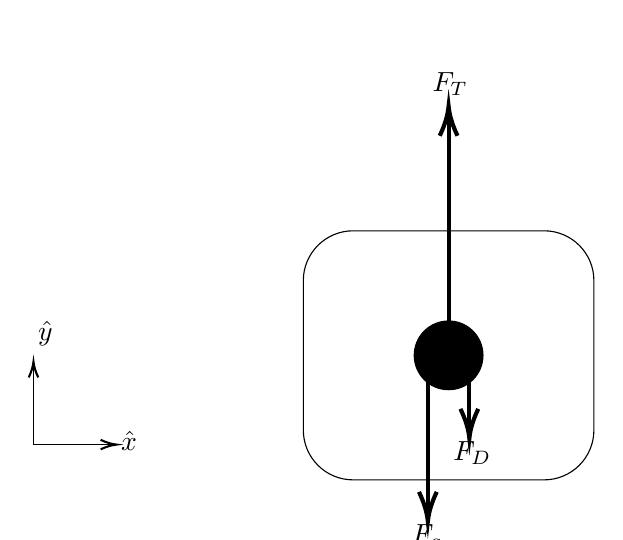
\begin{tikzpicture}[x=0.75pt,y=0.75pt,yscale=-1,xscale=1]
%uncomment if require: \path (0,308); %set diagram left start at 0, and has height of 308

%Rounded Rect [id:dp5842362308374554] 
\draw  [color={rgb, 255:red, 0; green, 0; blue, 0 }  ,draw opacity=1 ][fill={rgb, 255:red, 255; green, 255; blue, 255 }  ,fill opacity=1 ] (260,144) .. controls (260,130.75) and (270.75,120) .. (284,120) -- (376,120) .. controls (389.25,120) and (400,130.75) .. (400,144) -- (400,216) .. controls (400,229.25) and (389.25,240) .. (376,240) -- (284,240) .. controls (270.75,240) and (260,229.25) .. (260,216) -- cycle ;
%Straight Lines [id:da22630541270037763] 
\draw [line width=1.5]    (330,180) -- (330,63) ;
\draw [shift={(330,60)}, rotate = 90] [color={rgb, 255:red, 0; green, 0; blue, 0 }  ][line width=1.5]    (14.21,-4.28) .. controls (9.04,-1.82) and (4.3,-0.39) .. (0,0) .. controls (4.3,0.39) and (9.04,1.82) .. (14.21,4.28)   ;
%Straight Lines [id:da4912651471508729] 
\draw [line width=1.5]    (340,180) -- (340,217) ;
\draw [shift={(340,220)}, rotate = 270] [color={rgb, 255:red, 0; green, 0; blue, 0 }  ][line width=1.5]    (14.21,-4.28) .. controls (9.04,-1.82) and (4.3,-0.39) .. (0,0) .. controls (4.3,0.39) and (9.04,1.82) .. (14.21,4.28)   ;
%Shape: Circle [id:dp11471774870022611] 
\draw  [fill={rgb, 255:red, 0; green, 0; blue, 0 }  ,fill opacity=1 ] (313.44,180) .. controls (313.44,170.85) and (320.85,163.44) .. (330,163.44) .. controls (339.15,163.44) and (346.56,170.85) .. (346.56,180) .. controls (346.56,189.15) and (339.15,196.56) .. (330,196.56) .. controls (320.85,196.56) and (313.44,189.15) .. (313.44,180) -- cycle ;
%Straight Lines [id:da07105152032768414] 
\draw    (130,223) -- (130,185) ;
\draw [shift={(130,183)}, rotate = 90] [color={rgb, 255:red, 0; green, 0; blue, 0 }  ][line width=0.75]    (7.65,-2.3) .. controls (4.86,-0.97) and (2.31,-0.21) .. (0,0) .. controls (2.31,0.21) and (4.86,0.98) .. (7.65,2.3)   ;
%Straight Lines [id:da477096952774564] 
\draw    (130,223) -- (168,223) ;
\draw [shift={(170,223)}, rotate = 180] [color={rgb, 255:red, 0; green, 0; blue, 0 }  ][line width=0.75]    (7.65,-2.3) .. controls (4.86,-0.97) and (2.31,-0.21) .. (0,0) .. controls (2.31,0.21) and (4.86,0.98) .. (7.65,2.3)   ;
%Straight Lines [id:da5415789935745218] 
\draw [line width=1.5]    (320,180) -- (320,257) ;
\draw [shift={(320,260)}, rotate = 270] [color={rgb, 255:red, 0; green, 0; blue, 0 }  ][line width=1.5]    (14.21,-4.28) .. controls (9.04,-1.82) and (4.3,-0.39) .. (0,0) .. controls (4.3,0.39) and (9.04,1.82) .. (14.21,4.28)   ;

% Text Node
\draw (331,220.4) node [anchor=north west][inner sep=0.75pt]    {$F_{D}$};
% Text Node
\draw (321,42.4) node [anchor=north west][inner sep=0.75pt]    {$F_{T}$};
% Text Node
\draw (171,215.4) node [anchor=north west][inner sep=0.75pt]    {$\hat{x}$};
% Text Node
\draw (131,162.4) node [anchor=north west][inner sep=0.75pt]    {$\hat{y}$};
% Text Node
\draw (311,260.4) node [anchor=north west][inner sep=0.75pt]    {$F_{g}$};


\end{tikzpicture}
    \caption{1-DoF Forces on a body}
    \label{fig: 1DoF forces}
\end{figure}

In Figure \ref{fig: 1DoF forces}, a total of three forces are shown, all of which act along the $\hat{y}$-direction. The colinearity of all these forces is what makes this a 1-\gls{dof} model. The three forces shown are the thrust force, the drag force, and the gravity force.

Following what you may do in an introductory physics class, we will describe each of these forces via their functional form. These are described in Table \ref{force table}
$$
\begin{array}{cc}\label{force table}
    \mathrm{\textbf{Force}}&\mathrm{\textbf{Functional Form}}\\
    \vec{F}_g &  -mg\\
     \vec{F}_D& -\frac{1}{2} \rho_{\infty} V^2_{\infty}SC_D\\
     \vec{F}_T & F_T\cdot[1-u(t-t_b)], t\ge0
\end{array}
$$

\newglossaryentry{freestream}
{
    name=freestream,
    first = {\textit{freestream}},
    description={A freestream quantity is one that is far away from the body, such that the influences of the body are negligible. For example, freestream velocity is the velocity that would be seen outside the influence of the body at the same conditions}
}

\newglossaryentry{ref area}
{
    name=reference area,
    first = \textit{reference area},
    description={An area that is used to define a characteristic area of an object in aerodynamics. This is used to normalize quantities such as lift and drag}
    }

    \newglossaryentry{drag coeff}
{
    name=drag coefficient,
    first = \textit{drag coefficient},
    description={A non dimensional parameter that describes the amount of drag acting on an object. This non-dimensionalized value is given by $\frac{F_D}{q_{\infty}S}$, where $q_{\infty}$ is the dynamic pressure, $\frac{1}{2}\rho_{\infty}V_{\infty}^2$}
    }
The notation here is important to understand. In future AAE classes at Purdue, this is likely the notation that you will see. Terms with the subscript $\infty$ denote \gls{freestream} quantities, those that are freely flowing far away from the body of interest. Also of note is the unit step function, $u(t-t_b)$, which is a function which has value zero until reaching time $t_b$, where it thereafter equals one. The quantity  $\rho$ refers to the density of the fluid, and $S$ to the \gls{ref area}. The \gls{drag coeff} is $C_D$, a term which encapsulates the very complex nature of the fluid flow around an object. Calculating the value of $C_D$ will be explored more deeply in later sections of this document. For now, we may assume a constant value.

It is helpful to think about these quantities as vectors, because we can add them together to achieve a resultant.\footnote{More formally, we define this as a linear space, where multiplicative and additive properties are preserved. This formal definition allows us to apply this to any arbitrarily number of dimensions. } In the 1-dimensional case this is quite trivial since all vectors along the $\hat{y}$ unit vector, but this will become increasingly important as we move to higher dimensions.

\subsection{Numerical Integration in the 1-DoF}\label{sec: Numerical Integration in the 1DoF}
\newacronym{eom}{EOM}{Equation of Motion}
Now we will move into something that you may have not seen before. Given all the forces, we normally apply Newton’s 2\textsuperscript{nd} Law, $\sum{\vec{F}}=m\vec{a}$ , to arrive at an expression for the acceleration, known as an \gls{eom}, as shown in \eqref{eq2}. Doing so might look something like this:
\begin{gather}
F_T \cdot [1-u(t-t_b)]-\frac{1}{2}\rho_{\infty}V_{\infty}^2SC_D-mg=m\vec{a}\label{eq1} \\
\vec{a}=\frac{F_T \cdot [1-u(t-t_b)]-\frac{1}{2}\rho_{\infty}V_{\infty}^2SC_D}{m}-g\label{eq2}
\end{gather}
 From here, we use integration to find the velocity and then position of the object with time. Formally, we might define this formally as:
 $$\vec{V}=\int{\vec{a}}{dt}$$
However, you may notice something strange with our equation. In our expression for acceleration, we need to know the velocity. However, we do not know the velocity without integrating the equation first. Since this dependence is non-linear, this becomes even more complicated to solve. This puts us in a chicken v. egg situation, so we must take a different approach to the problem. \footnote{Sometimes systems like this can be solved with traditional ODE methods. However, most complex systems like our 6-\gls{dof} have no known analytical solutions. We will focus on numerical integration because it will be more useful in general. }

\newglossaryentry{numerical int}
{
    name=numerical integration,
    first = {\textit{numerical integration}},
    description={The process of making a numerical approximation of a differential equation through discretization of the independent variable (usually time for most physical phenomenon)}
}

The way we resolve this is to make an approximation of the solution in a process called \gls{numerical int}. Here, we will outline the simplest type of numerical integration, known as Euler’s Method. This section aims to show how to implement Euler’s method in code, and the mathematical reasoning will be given a more formal treatment in Section \ref{sec:euler integration}. We will describe more complex numerical integration schemes and why you might want to use them, but it’s good to see the code for a simple case first.

Euler’s Method involves discretizing our time interval. You may remember the concept of a Riemann sum from calculus, where you approximate an integral in discrete time steps. We will take a similar approach with Euler’s Method. Euler’s method is applicable to solving first order ordinary differential equations (ODE’s). However, in our problem, we have a second order differential equation, because $\vec{a}=\ddot{y}$.

To resolve this issue, we will make this one differential equation into a system of first-order differential equations. In general, we can convert an nth-order ODE into a system of n first-order ODEs.

In this case, we define a variable, $v=\dot{y}$. Now, we can express equation \eqref{eq2} as a system of two differential equations:

\begin{gather}\label{system}
        \dot{v}=\frac{F_T \cdot [1-u(t-t_b)]-\frac{1}{2}\rho_{\infty}V_{\infty}^2SC_D}{m}-g\\
    \dot{y}=v
\end{gather}
Now, we will apply Euler’s method to solve the problem. We will use the following steps to do so, using equation \eqref{system} as our example:

1. Rewrite the system in Leibniz notation, where $\dot{x}=\frac{dx}{dt}$.

2. Perform separation of variables, to arrive at $dx=v\cdot dt$.

3. Discretize the equation by ‘converting’  $dx$ and $dt$ to $\Delta x$ and $\Delta t$.\footnote{Note that we are not ‘converting’ in the sense of an equality, since the equations are no longer equivalent when we convert a differential element into a discrete one. We are just making an approximation of the true solution. Luckily, numerical integration schemes can get us quite close to true solutions. }

4. Rewrite $\Delta x$ as $x_{new}-x_{old}$. We can rearrange the equation as $x_{new}=v\cdot \Delta t + x_{old}$

5. To start, we define an initial state. This initial state will be the first value of $x_{old}$. 

6. Iterate through values of $\Delta t$ until the desired time of simulation is achieved.

We follow the same process for the integration of acceleration to find the velocity. Of note, we will use the previous value of $\vec{v}$ in the computation of the new acceleration. Note that a more formal definition of Euler’s method is given in Section \ref{sec:euler integration}.

We also show this example in MATLAB Script \ref{Script 1} below. Note that $\frac{1}{2}\rho_{\infty}SC_D$ is called $k$ in the script for simplicity. This simplification assumes that $\rho_{\infty}$ and the $C_D$ are constant, which we will later see is a quite poor assumption but is okay for a first approximation.

\lstset{style=mystyle}

\lstinputlisting[language=Matlab, caption=1 DoF]{6DoF Explanation Scripts/OneDofEuler.m}\label{Script 1}

There are a few important things to note about the MATLAB implementation of the script. Firstly, the only force that is defined outside of the loop is gravity, because the magnitude and direction of this force is independent of the current state of the system. We contrast this with the drag force and the thrust, which must be calculated on every iteration through the algorithm to find an updated value for the force.

We also note the use of the "heaviside" function. This is functionally identical to a unit step function, just a different notation.

\section{Frame of Reference}\label{sec:Frame of Reference}
Before attempting to describe movement in multiple dimensions, we should first discuss how we can describe important quantities through different lenses. Later, it will become apparent that a vector or problem is easier described or completed through one lens than another. We call these different lenses reference frames.

\newglossaryentry{orthonormal}
{
    name=orthonormal,
    first = {\textit{orthonormal}},
    description={A set of basis vectors that are mutually orthogonal to each other in a vector space and have unit length. We mostly refer to orthonormal vectors in $\mathbb{R}^3$ space}
}

A frame of reference is an \gls{orthonormal} set within three-dimensional space. The \gls{orthonormal} nature of the basis vectors that create every frame of reference allows for any other vector in 3-dimensional space to be described as a linear combination of those three basis vectors (hence why we call it a basis for 3-space). This tool becomes incredibly useful within the study of Newtonian and Attitude Dynamics, as every arbitrary vector can be broken down into three set ''scalar'' directions. Naturally, the question arises of how we determine which set directions to utilize, and so we will be discussing a few frames of reference critical to the creation of a 6-\gls{dof} and Aerospace engineering as a whole.
\subsection{The Inertial Frame}

\newglossaryentry{inertial frame}
{
    name=inertial frame,
    first = {\textit{inertial frame}},
    description={A reference frame that is static and experiences no accelerations. We use the Earth's surface as the reference frame for our rocket.}
}

The first and most important frame of reference is the \gls{inertial frame}. Typically denoted by $e$ or $i$, or in our case $(\hat{x},\hat{y},\hat{z})$, this motionless frame is the one that allows for the use of Newton’s second law in the first place, as the frame itself has ''zero'' translational and rotational movement.\footnote{An inertial frame can have some constant velocity and still be inertial. Of course, the earth has some velocity around the sun and with respect to the distant stars which we can approximate as constant for our time scales and thus ignore.} We say “zero” as this motion must be negligible in relation to the vehicle of interest. For example, this specific 6-\gls{dof} sets the inertial frame to be anchored within the Earth on the launch pad. And while we are well aware the Earth is moving and rotating through space at a non-zero rate, this motion is negligible relative to the motion of our vehicle which remains close to Earth within the atmosphere for a short period of time. Therefore, we can assume that the Earth acts appropriately as an inertial frame of reference, and Newton’s second law is valid for this frame. 

\newacronym{rhr}{RHR}{right hand rule}

Returning to the specific example of a 6-\gls{dof}, the directions you set your basis vectors to point in are mostly left to the coder’s discretion. If your chosen directions retain the orthonormal nature of a frame of reference, as well as obeying the \gls{rhr}, the choice is all yours. Within the example we are following, our inertial frame’s origin is anchored within the launch pad as previously stated. The first inertial basis vector points up perpendicular to the Earth’s surface, the second inertial basis vector points due East, while the third inertial basis vector follows the right-hand rule and points due North. An image for quick reference is provided in Figure \ref{fig:InertialFrame}:

\begin{figure}[H]
\centering
\tikzset{every picture/.style={line width=0.75pt}} %set default line width to 0.75pt        
\begin{tikzpicture}[x=0.75pt,y=0.75pt,yscale=-1,xscale=1]
%uncomment if require: \path (0,356); %set diagram left start at 0, and has height of 356

%Shape: Axis 2D [id:dp4662897481397581] 
\draw  (244,205.18) -- (448.8,205.18)(264.48,52) -- (264.48,222.2) (441.8,200.18) -- (448.8,205.18) -- (441.8,210.18) (259.48,59) -- (264.48,52) -- (269.48,59)  ;
%Straight Lines [id:da8652713079639678] 
\draw    (278.8,190.2) -- (174.38,299.55) ;
\draw [shift={(173,301)}, rotate = 313.68] [color={rgb, 255:red, 0; green, 0; blue, 0 }  ][line width=0.75]    (10.93,-3.29) .. controls (6.95,-1.4) and (3.31,-0.3) .. (0,0) .. controls (3.31,0.3) and (6.95,1.4) .. (10.93,3.29)   ;
%Shape: Circle [id:dp9817397826908267] 
\draw  [fill={rgb, 255:red, 0; green, 0; blue, 0 }  ,fill opacity=1 ] (259.08,205.18) .. controls (259.08,202.2) and (261.5,199.78) .. (264.48,199.78) .. controls (267.46,199.78) and (269.88,202.2) .. (269.88,205.18) .. controls (269.88,208.16) and (267.46,210.58) .. (264.48,210.58) .. controls (261.5,210.58) and (259.08,208.16) .. (259.08,205.18) -- cycle ;

% Text Node
\draw (242,9) node [anchor=north west][inner sep=0.75pt]   [align=left] {Upward};
% Text Node
\draw (253,27.4) node [anchor=north west][inner sep=0.75pt]    {$\hat{x} ,\hat{e}_{1}$};
% Text Node
\draw (154,300.4) node [anchor=north west][inner sep=0.75pt]    {$\hat{y} ,\hat{e}_{2}$};
% Text Node
\draw (151,325) node [anchor=north west][inner sep=0.75pt]   [align=left] {East};
% Text Node
\draw (453,187.4) node [anchor=north west][inner sep=0.75pt]    {$\hat{z} ,\hat{e}_{3}$};
% Text Node
\draw (448,211) node [anchor=north west][inner sep=0.75pt]   [align=left] {North};
% Text Node
\draw (271.89,208.15) node [anchor=north west][inner sep=0.75pt]  [rotate=-0.04] [align=left] {Launchpad};


\end{tikzpicture}
    \caption{Inertial Frame Convention}
    \label{fig:InertialFrame}
\end{figure}

\subsection{The Body Frame}

\newglossaryentry{body frame}
{
    name=body frame,
    first = {\textit{body frame}},
    description={A reference frame that is fixed to the body of an object and follows the translations and rotations of the vehicle}
}

The second most important frame of reference is the \gls{body frame}. Typically denoted by $b$, or in our case $(\hat{X},\hat{Y},\hat{Z})$, this frame of reference is always anchored at some point in the vehicle and allows us to describe the \gls{state vector} in relation to the vehicle itself. This frame is moving and rotating with respect to the inertial frame. For every body frame you create – from a frame for the entire vehicle to a frame for a small electronic part – you want simplicity. This means that in aerospace, it is often the case for a general \gls{body frame} to have a basis vector pointing along the longitudinal axis of the vehicle, as well as one out a wing. A generic image of such a convention is provided in Figure\ref{fig:BodyFrameTypical} In addition, it means at a zero angle of rotation, every basis vector of the body frame is parallel to the corresponding basis vector in the inertial frame. This is imperative to rotational dynamics, as the offset of each basis vector in the \gls{body frame} will correspond to the pitch, yaw, and roll of the vehicle. But more on that in Volume II.

% Either change or give credit to MATLAB ig

\begin{figure}[H]
\centering
    
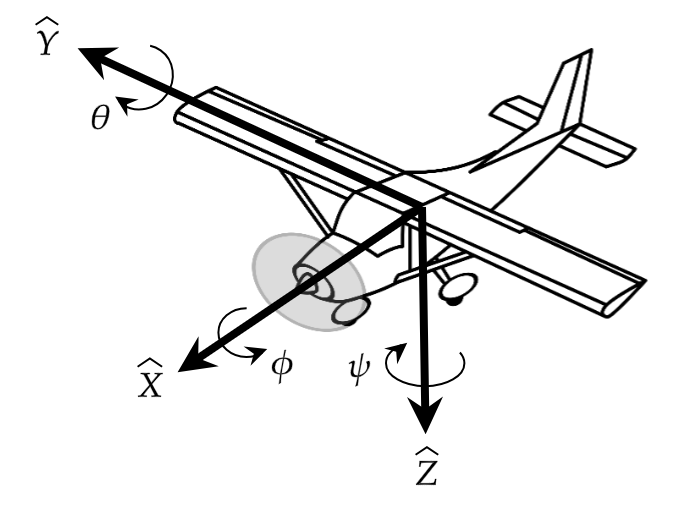
\includegraphics[width=\linewidth]{Images/TypicalBodyFrame.png}
    \caption{Typical Body Frame Orientation}
    \label{fig:BodyFrameTypical}
\end{figure}

For our current model, the body frame of our 6-\gls{dof} has its origin in the nose of the vehicle. It has the first body basis vector, $\hat{X}$, pointing up along the longitudinal axis of the rocket following standard convention. The second basis vector, $\hat{Y}$, points right due East when on the launch pad, and the third, $\hat{Z}$, points due North on the launch pad. We use the cardinal directions of the launchpad as not only are there no conventional wings on the rocket, but it allows body frame to be defined parallel to the corresponding inertial frame basis vectors. Note that they won’t remain pointing in these directions as the rocket moves through space, and they may not even begin parallel to the inertial axis to begin with if the rocket launches from a tilt.

\begin{figure}[H]
\centering
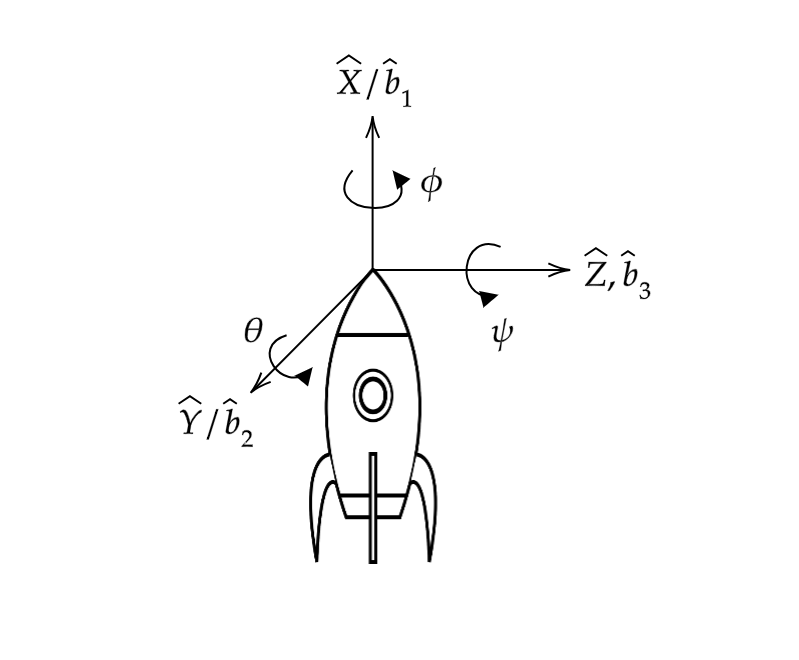
\includegraphics[width=\linewidth]{Images/RocketBodyFrame.png}
    \caption{Body Frame Convention of our Rocket}
    \label{fig:BodyFrameRocket}
\end{figure}

\subsection{The Wind Frame}

\newglossaryentry{wind frame}
{
    name=wind frame,
    first = {\textit{wind frame}},
    description={A reference frame in reference to the direction of freestream velocity, denoted $V_{\infty}$}
}

The last and by far least important frame of reference is the \gls{wind frame}. This frame of reference, like the body frame, is always anchored at some point in the vehicle. Also like the body frame, it moves and rotates with the vehicle and allows for a new way of describing the \gls{state vector}. Unlike the body frame, the most important definition is not along the longitudinal axis of the vehicle. As indicated by its name, the necessary orientation of a basis vector points in the direction of the free stream velocity. Relating this to the body frame, this translates to an offset from the body frame by the \gls{angle of attack} and sideslip. This frame is often useful for aircraft, but we do not use it explicitly in our 6-\gls{dof}. The wind frame itself is in fact skipped over during wind calculations, as the \gls{angle of attack} and imparted forces/moments are calculated directly onto the body frame. So as this isn’t as useful as the other two reference frames, we won’t elaborate on this frame any further, and it won’t be shown as much in our example 6-\gls{dof}.

\section{The 3-DoF Case}\label{sec: 3DoF Case}
\subsection{Vectors in the 3-DoF Case}
For particle dynamics, the most complex case is full 3D translational motion. Luckily, nothing very fundamental changes as compared to the 1-\gls{dof} case. The most important difference is the use of vector notation for compactness and clarity of mathematics and code. For position ($\vec{r}$), velocity ($\vec {v}$), and acceleration ($\vec{a}$), we represent them as tri-dimensional column vectors:

\begin{gather}
    \vec{r}=\begin{bmatrix}
        x_1\\
        x_2\\
        x_3
    \end{bmatrix},
    \vec{v}=\begin{bmatrix}
        \dot{x}_1\\
        \dot{x}_2\\
        \dot{x}_3\\
    \end{bmatrix},
        \vec{a}=\begin{bmatrix}
        \ddot{x}_1\\
        \ddot{x}_2\\
        \ddot{x}_3\\
    \end{bmatrix}
\end{gather}
This is done not only for the sake of compactness, but also to facilitate the use of matrix operations for translation between reference frames. This concept is further explored in Section \ref{sec:Frame of Reference}. For this reason, expressing these elements in vector form will become crucial as we move forward. In MATLAB, we express a tri-dimensional column vector as:
\begin{lstlisting}[language=Matlab]
pos=[0;0;0];
\end{lstlisting}
Where each semicolon represents a new row of the vector. We define a row vector by using a comma instead of a semicolon: 
\begin{lstlisting}[language=Matlab]
pos=[0,0,0];
\end{lstlisting}
Often, it is useful to convert between a row and column vector in MATLAB because some functions will expect the input to be in a different format. We can do so with a transposition. In MATLAB, this looks like: 
\begin{lstlisting}
pos=[0,0,0]';
\end{lstlisting}
Expressed in vector notation, we write Newton's 2nd Law in the 3D case as $\vec{F}=m{}^i\ddot{\vec{r}}^{\ op}$. The presence of $i$ indicates that this acceleration vector must be in the inertial frame. The quantity ${}^i\ddot{\vec{r}}^{\ op}$ can be deduced from the use of the \gls{bke} in simple cases.

\subsection{Vector directions in the 3-DoF}\label{sec: vector directions in the 3DoF}
We present below a modified version of the 1-\gls{dof} below in full 3D in Figure \ref{fig:3 DoF Forces}.

\tikzset{every picture/.style={line width=0.75pt}} %set default line width to 0.75pt       

\begin{figure}[ht]
    \centering
    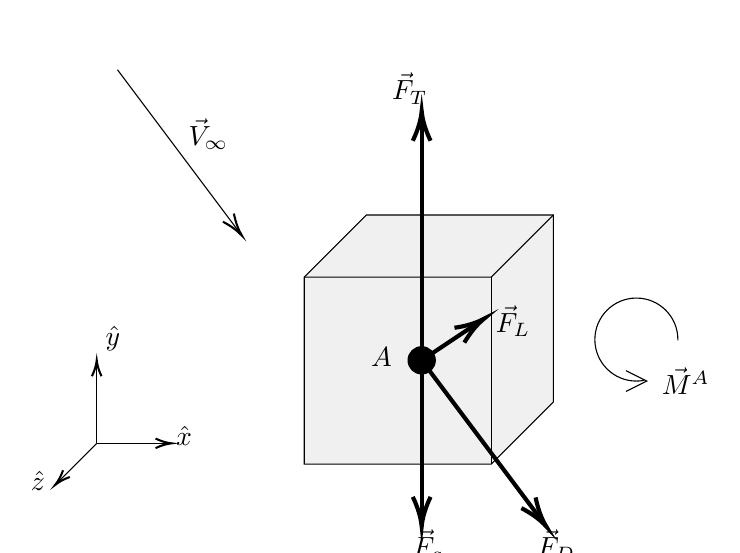
\begin{tikzpicture}[x=0.75pt,y=0.75pt,yscale=-1,xscale=1]
%uncomment if require: \path (0,308); %set diagram left start at 0, and has height of 308

%Shape: Cube [id:dp15885218660825062] 
\draw  [fill={rgb, 255:red, 155; green, 155; blue, 155 }  ,fill opacity=0.15 ] (260,129.92) -- (289.92,100) -- (380,100) -- (380,190.08) -- (350.08,220) -- (260,220) -- cycle ; \draw   (380,100) -- (350.08,129.92) -- (260,129.92) ; \draw   (350.08,129.92) -- (350.08,220) ;
%Straight Lines [id:da7537274804871096] 
\draw    (160,210) -- (160,172) ;
\draw [shift={(160,170)}, rotate = 90] [color={rgb, 255:red, 0; green, 0; blue, 0 }  ][line width=0.75]    (7.65,-2.3) .. controls (4.86,-0.97) and (2.31,-0.21) .. (0,0) .. controls (2.31,0.21) and (4.86,0.98) .. (7.65,2.3)   ;
%Straight Lines [id:da28051238395124845] 
\draw    (160,210) -- (194,210) ;
\draw [shift={(196,210)}, rotate = 180] [color={rgb, 255:red, 0; green, 0; blue, 0 }  ][line width=0.75]    (7.65,-2.3) .. controls (4.86,-0.97) and (2.31,-0.21) .. (0,0) .. controls (2.31,0.21) and (4.86,0.98) .. (7.65,2.3)   ;
%Straight Lines [id:da0491508391303197] 
\draw    (160,210) -- (141.41,228.59) ;
\draw [shift={(140,230)}, rotate = 315] [color={rgb, 255:red, 0; green, 0; blue, 0 }  ][line width=0.75]    (7.65,-2.3) .. controls (4.86,-0.97) and (2.31,-0.21) .. (0,0) .. controls (2.31,0.21) and (4.86,0.98) .. (7.65,2.3)   ;
%Straight Lines [id:da4424478744689285] 
\draw    (170,30) -- (228.8,108.4) ;
\draw [shift={(230,110)}, rotate = 233.13] [color={rgb, 255:red, 0; green, 0; blue, 0 }  ][line width=0.75]    (10.93,-3.29) .. controls (6.95,-1.4) and (3.31,-0.3) .. (0,0) .. controls (3.31,0.3) and (6.95,1.4) .. (10.93,3.29)   ;
%Straight Lines [id:da9341165159771404] 
\draw [line width=1.5]    (316.56,170) -- (316.56,247) ;
\draw [shift={(316.56,250)}, rotate = 270] [color={rgb, 255:red, 0; green, 0; blue, 0 }  ][line width=1.5]    (14.21,-4.28) .. controls (9.04,-1.82) and (4.3,-0.39) .. (0,0) .. controls (4.3,0.39) and (9.04,1.82) .. (14.21,4.28)   ;
%Straight Lines [id:da4700324062294746] 
\draw [line width=1.5]    (316.56,170) -- (374.76,247.6) ;
\draw [shift={(376.56,250)}, rotate = 233.13] [color={rgb, 255:red, 0; green, 0; blue, 0 }  ][line width=1.5]    (14.21,-4.28) .. controls (9.04,-1.82) and (4.3,-0.39) .. (0,0) .. controls (4.3,0.39) and (9.04,1.82) .. (14.21,4.28)   ;
%Straight Lines [id:da6206056974950449] 
\draw [line width=1.5]    (316.56,170) -- (316.56,53) ;
\draw [shift={(316.56,50)}, rotate = 90] [color={rgb, 255:red, 0; green, 0; blue, 0 }  ][line width=1.5]    (14.21,-4.28) .. controls (9.04,-1.82) and (4.3,-0.39) .. (0,0) .. controls (4.3,0.39) and (9.04,1.82) .. (14.21,4.28)   ;
%Shape: Circle [id:dp9278618893074794] 
\draw  [fill={rgb, 255:red, 0; green, 0; blue, 0 }  ,fill opacity=1 ] (310,170) .. controls (310,166.38) and (312.94,163.44) .. (316.56,163.44) .. controls (320.19,163.44) and (323.13,166.38) .. (323.13,170) .. controls (323.13,173.62) and (320.19,176.56) .. (316.56,176.56) .. controls (312.94,176.56) and (310,173.62) .. (310,170) -- cycle ;
%Straight Lines [id:da05847350311292765] 
\draw [line width=1.5]    (316.56,170) -- (344.07,151.66) ;
\draw [shift={(346.56,150)}, rotate = 146.31] [color={rgb, 255:red, 0; green, 0; blue, 0 }  ][line width=1.5]    (14.21,-4.28) .. controls (9.04,-1.82) and (4.3,-0.39) .. (0,0) .. controls (4.3,0.39) and (9.04,1.82) .. (14.21,4.28)   ;
%Shape: Arc [id:dp5580370574812169] 
\draw  [draw opacity=0] (423.67,179.66) .. controls (422.48,179.88) and (421.25,180) .. (420,180) .. controls (408.95,180) and (400,171.05) .. (400,160) .. controls (400,148.95) and (408.95,140) .. (420,140) .. controls (431.05,140) and (440,148.95) .. (440,160) .. controls (440,160.15) and (440,160.29) .. (440,160.44) -- (420,160) -- cycle ; \draw   (423.67,179.66) .. controls (422.48,179.88) and (421.25,180) .. (420,180) .. controls (408.95,180) and (400,171.05) .. (400,160) .. controls (400,148.95) and (408.95,140) .. (420,140) .. controls (431.05,140) and (440,148.95) .. (440,160) .. controls (440,160.15) and (440,160.29) .. (440,160.44) ;  
\draw   (415,175) -- (425,180) -- (415,185) ;

% Text Node
\draw (197,200.4) node [anchor=north west][inner sep=0.75pt]    {$\hat{x}$};
% Text Node
\draw (163,152.4) node [anchor=north west][inner sep=0.75pt]    {$\hat{y}$};
% Text Node
\draw (127,222.4) node [anchor=north west][inner sep=0.75pt]    {$\hat{z}$};
% Text Node
\draw (203,52.4) node [anchor=north west][inner sep=0.75pt]    {$\vec{V}_{\infty }$};
% Text Node
\draw (311,250.4) node [anchor=north west][inner sep=0.75pt]    {$\vec{F}_{g}$};
% Text Node
\draw (371,250.4) node [anchor=north west][inner sep=0.75pt]    {$\vec{F}_{D}$};
% Text Node
\draw (301,30.4) node [anchor=north west][inner sep=0.75pt]    {$\vec{F}_{T}$};
% Text Node
\draw (351,142.4) node [anchor=north west][inner sep=0.75pt]    {$\vec{F}_{L}$};
% Text Node
\draw (431,172.4) node [anchor=north west][inner sep=0.75pt]    {$\vec{M}^{A}$};
% Text Node
\draw (291,162.4) node [anchor=north west][inner sep=0.75pt]    {$A$};


\end{tikzpicture}

    \caption{3-DoF Forces on a Body}
    \label{fig:3 DoF Forces}
\end{figure}
\newglossaryentry{angle of attack}
{
    name=angle of attack,
    first={\textit{angle of attack}},
    description={The angle of offset of the freestream velocity with the $\hat{X}$/$\hat{b}_1$, or longitudinal axis, of the vehicle. This is often denoted with the Greek letter $\alpha$}
}
As compared to 1-\gls{dof} case, we have three new quantities that are present. The first of these is $\vec{V}_{\infty}$, the freestream airflow vector.\footnote{\gls{freestream} velocity  is drawn in the direction of incoming air by convention. However, for calculations, we will use the convention that  is the direction of the velocity of the vehicle (opposite sign to drawing).} This is represented diagrammatically because it is no longer constrained along the $\hat{y}$ direction. When we have an angle between the nose (the direction through which the thrust force points in Figure \ref{fig:3 DoF Forces}) and the \gls{freestream} velocity, we refer to this as an \gls{angle of attack}. This \gls{angle of attack} is often denoted with the letter $\alpha$. We will discuss \gls{angle of attack} and its effects more in Section \ref{sec: aerodynamics}. For now, we simply need to understand how to calculate $\alpha$ given the vector through the nose and the \gls{freestream} velocity vector.

To do this, we use the fact that the dot product is related to the cosine of the angle between the vectors. Denoting the vector through the nose of the rocket $\hat{X}$, we can find the \gls{angle of attack} as:
\begin{equation}\label{eq:alpha}
    \alpha=cos^{-1}\left(\frac{\hat{X}\cdot \vec{V}_{\infty}}{||\hat{X}||\ ||\vec{V}_{\infty}||}\right)
\end{equation}

The next new quantity is $\vec{F}_L$, the force of lift. The force of lift is always perpendicular in direction to $\vec{V}_{\infty}$. Knowing this, we can find the direction of the force of lift as:
\begin{equation}\label{eq:Lift}
    \hat{L}=\frac{(\hat{V}_{\infty} \times \hat{X}) \times \hat{V}_{\infty}}{||(\hat{V}_{\infty} \times \hat{X}) \times \hat{V}_{\infty}||}
\end{equation}
Here, the cross product is used because it generates a vector orthogonal to the two input vectors. This is exactly the property that we need when defining lift.

For the sake of completeness, we should also note that the force of drag lies opposite the direction of $\vec{V}_{\infty}$. This is much simpler to calculate, and looks like:
\begin{equation}\label{eq:drag}
\hat{D}=\frac{-\vec{V}_{\infty}}{||\vec{V}_{\infty}||}
\end{equation}
The last force directions to define are the direction of thrust and the direction of gravity. Luckily, these are easily defined because they point directly along basis vectors.\footnote{We assume here that there is no misalignment in the thrust vector and it is coincident with the  vector.} The force of gravity is defined with respect to the inertial reference frame and is defined in \eqref{eq:Fg}. The force of thrust is defined with respect to the vector pointing through the nose, $\hat{X}$, and is shown in \eqref{eq:Ft}:
\begin{equation}\label{eq:Fg}
    \vec{F}_g=-mg\cdot \hat{y}
\end{equation}
\begin{equation}\label{eq:Ft}
    \vec{F}_T=F_T\cdot \hat{X}
\end{equation}
\subsection{Moments}\label{sec:moments}
The last new quantity is the moment about point A, denoted $\vec{M}^A$. For now, we will simply note that for an arbitrary selection of point A, we will have a rotational moment that is generated because the forces on the body do not necessarily act through point A, even if it is the center of mass (see section 4 for more details). In Figure\ref{fig:3 DoF Forces}, we have drawn all of the forces acting through a single point for simplicity, but this is not generally the case.

For our rocket modeling, it is generally assumed that gravity and thrust act about the center of gravity, and the aerodynamic forces about the center of pressure.

We will show how to compute this moment if the location of the center of gravity and the center of pressure is known. To show this, we will briefly return to the 2D case for illustration, but keep in mind that this concept is extensible in 3D. We show this in Figure \ref{fig:Moments}.

\begin{figure}[ht]
    \centering
    
\tikzset{every picture/.style={line width=0.75pt}} %set default line width to 0.75pt        

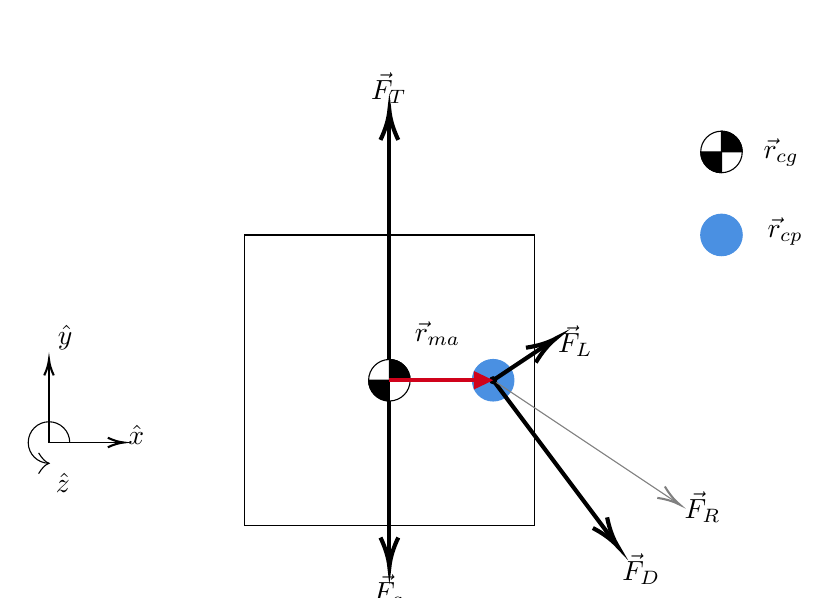
\begin{tikzpicture}[x=0.75pt,y=0.75pt,yscale=-1,xscale=1]
%uncomment if require: \path (0,300); %set diagram left start at 0, and has height of 300

%Shape: Rectangle [id:dp16059631350753278] 
\draw   (224,90) -- (364,90) -- (364,230) -- (224,230) -- cycle ;
%Shape: Circle [id:dp26152316559967836] 
\draw   (284,160) .. controls (284,154.48) and (288.48,150) .. (294,150) .. controls (299.52,150) and (304,154.48) .. (304,160) .. controls (304,165.52) and (299.52,170) .. (294,170) .. controls (288.48,170) and (284,165.52) .. (284,160) -- cycle ;
%Straight Lines [id:da4396178512453982] 
\draw [line width=1.5]    (294,150) -- (294,33) ;
\draw [shift={(294,30)}, rotate = 90] [color={rgb, 255:red, 0; green, 0; blue, 0 }  ][line width=1.5]    (14.21,-4.28) .. controls (9.04,-1.82) and (4.3,-0.39) .. (0,0) .. controls (4.3,0.39) and (9.04,1.82) .. (14.21,4.28)   ;
%Straight Lines [id:da6367078669315451] 
\draw [line width=1.5]    (294,170) -- (294,247) ;
\draw [shift={(294,250)}, rotate = 270] [color={rgb, 255:red, 0; green, 0; blue, 0 }  ][line width=1.5]    (14.21,-4.28) .. controls (9.04,-1.82) and (4.3,-0.39) .. (0,0) .. controls (4.3,0.39) and (9.04,1.82) .. (14.21,4.28)   ;
%Shape: Circle [id:dp9868324677149697] 
\draw  [color={rgb, 255:red, 74; green, 144; blue, 226 }  ,draw opacity=1 ][fill={rgb, 255:red, 74; green, 144; blue, 226 }  ,fill opacity=1 ] (334,160) .. controls (334,154.48) and (338.48,150) .. (344,150) .. controls (349.52,150) and (354,154.48) .. (354,160) .. controls (354,165.52) and (349.52,170) .. (344,170) .. controls (338.48,170) and (334,165.52) .. (334,160) -- cycle ;
%Straight Lines [id:da08375154983020605] 
\draw [line width=1.5]    (344,160) -- (371.5,141.66) ;
\draw [shift={(374,140)}, rotate = 146.31] [color={rgb, 255:red, 0; green, 0; blue, 0 }  ][line width=1.5]    (14.21,-4.28) .. controls (9.04,-1.82) and (4.3,-0.39) .. (0,0) .. controls (4.3,0.39) and (9.04,1.82) .. (14.21,4.28)   ;
%Straight Lines [id:da9997269035553926] 
\draw [line width=1.5]    (344,160) -- (402.2,237.6) ;
\draw [shift={(404,240)}, rotate = 233.13] [color={rgb, 255:red, 0; green, 0; blue, 0 }  ][line width=1.5]    (14.21,-4.28) .. controls (9.04,-1.82) and (4.3,-0.39) .. (0,0) .. controls (4.3,0.39) and (9.04,1.82) .. (14.21,4.28)   ;
%Straight Lines [id:da3915949331033487] 
\draw [color={rgb, 255:red, 128; green, 128; blue, 128 }  ,draw opacity=1 ]   (344,160) -- (432.34,218.89) ;
\draw [shift={(434,220)}, rotate = 213.69] [color={rgb, 255:red, 128; green, 128; blue, 128 }  ,draw opacity=1 ][line width=0.75]    (10.93,-3.29) .. controls (6.95,-1.4) and (3.31,-0.3) .. (0,0) .. controls (3.31,0.3) and (6.95,1.4) .. (10.93,3.29)   ;
%Shape: Circle [id:dp6233406826761347] 
\draw  [fill={rgb, 255:red, 0; green, 0; blue, 0 }  ,fill opacity=1 ] (342.33,160) .. controls (342.33,159.08) and (343.08,158.33) .. (344,158.33) .. controls (344.92,158.33) and (345.67,159.08) .. (345.67,160) .. controls (345.67,160.92) and (344.92,161.67) .. (344,161.67) .. controls (343.08,161.67) and (342.33,160.92) .. (342.33,160) -- cycle ;
%Shape: Pie [id:dp5263153723129019] 
\draw  [fill={rgb, 255:red, 0; green, 0; blue, 0 }  ,fill opacity=1 ] (294,150) .. controls (294,150) and (294,150) .. (294,150) .. controls (299.52,150) and (304,154.48) .. (304,160) -- (294,160) -- cycle ;
%Shape: Pie [id:dp03519524739615432] 
\draw  [fill={rgb, 255:red, 0; green, 0; blue, 0 }  ,fill opacity=1 ] (294,170) .. controls (294,170) and (294,170) .. (294,170) .. controls (294,170) and (294,170) .. (294,170) .. controls (288.48,170) and (284,165.52) .. (284,160) -- (294,160) -- cycle ;
%Straight Lines [id:da5638933773253405] 
\draw [color={rgb, 255:red, 208; green, 2; blue, 27 }  ,draw opacity=1 ][line width=1.5]    (294,160) -- (340,160) ;
\draw [shift={(344,160)}, rotate = 180] [fill={rgb, 255:red, 208; green, 2; blue, 27 }  ,fill opacity=1 ][line width=0.08]  [draw opacity=0] (9.29,-4.46) -- (0,0) -- (9.29,4.46) -- cycle    ;
%Shape: Circle [id:dp854204209250383] 
\draw   (444,50) .. controls (444,44.48) and (448.48,40) .. (454,40) .. controls (459.52,40) and (464,44.48) .. (464,50) .. controls (464,55.52) and (459.52,60) .. (454,60) .. controls (448.48,60) and (444,55.52) .. (444,50) -- cycle ;
%Shape: Pie [id:dp5370740069872785] 
\draw  [fill={rgb, 255:red, 0; green, 0; blue, 0 }  ,fill opacity=1 ] (454,60) .. controls (454,60) and (454,60) .. (454,60) .. controls (454,60) and (454,60) .. (454,60) .. controls (448.48,60) and (444,55.52) .. (444,50) -- (454,50) -- cycle ;
%Shape: Pie [id:dp7640770799900009] 
\draw  [fill={rgb, 255:red, 0; green, 0; blue, 0 }  ,fill opacity=1 ] (454,40) .. controls (454,40) and (454,40) .. (454,40) .. controls (459.52,40) and (464,44.48) .. (464,50) -- (454,50) -- cycle ;
%Shape: Circle [id:dp281241699306923] 
\draw  [color={rgb, 255:red, 74; green, 144; blue, 226 }  ,draw opacity=1 ][fill={rgb, 255:red, 74; green, 144; blue, 226 }  ,fill opacity=1 ] (444,90) .. controls (444,84.48) and (448.48,80) .. (454,80) .. controls (459.52,80) and (464,84.48) .. (464,90) .. controls (464,95.52) and (459.52,100) .. (454,100) .. controls (448.48,100) and (444,95.52) .. (444,90) -- cycle ;
%Straight Lines [id:da2704614420307284] 
\draw    (130,190) -- (130,152) ;
\draw [shift={(130,150)}, rotate = 90] [color={rgb, 255:red, 0; green, 0; blue, 0 }  ][line width=0.75]    (7.65,-2.3) .. controls (4.86,-0.97) and (2.31,-0.21) .. (0,0) .. controls (2.31,0.21) and (4.86,0.98) .. (7.65,2.3)   ;
%Straight Lines [id:da24091737468013485] 
\draw    (130,190) -- (164,190) ;
\draw [shift={(166,190)}, rotate = 180] [color={rgb, 255:red, 0; green, 0; blue, 0 }  ][line width=0.75]    (7.65,-2.3) .. controls (4.86,-0.97) and (2.31,-0.21) .. (0,0) .. controls (2.31,0.21) and (4.86,0.98) .. (7.65,2.3)   ;
%Shape: Arc [id:dp6249807559731687] 
\draw  [draw opacity=0] (130,200) .. controls (130,200) and (130,200) .. (130,200) .. controls (130,200) and (130,200) .. (130,200) .. controls (124.48,200) and (120,195.52) .. (120,190) .. controls (120,184.48) and (124.48,180) .. (130,180) .. controls (135.52,180) and (140,184.48) .. (140,190) -- (130,190) -- cycle ; \draw   (130,200) .. controls (130,200) and (130,200) .. (130,200) .. controls (130,200) and (130,200) .. (130,200) .. controls (124.48,200) and (120,195.52) .. (120,190) .. controls (120,184.48) and (124.48,180) .. (130,180) .. controls (135.52,180) and (140,184.48) .. (140,190) ;  
\draw   (125,195) .. controls (126.67,197.78) and (128.33,199.44) .. (130,200) .. controls (128.33,200.56) and (126.67,202.22) .. (125,205) ;

% Text Node
\draw (284,10.4) node [anchor=north west][inner sep=0.75pt]    {$\vec{F}_{T}$};
% Text Node
\draw (285,252.4) node [anchor=north west][inner sep=0.75pt]    {$\vec{F}_{g}$};
% Text Node
\draw (374,132.4) node [anchor=north west][inner sep=0.75pt]    {$\vec{F}_{L}$};
% Text Node
\draw (405,242.4) node [anchor=north west][inner sep=0.75pt]    {$\vec{F}_{D}$};
% Text Node
\draw (435,212.4) node [anchor=north west][inner sep=0.75pt]    {$\vec{F}_{R}$};
% Text Node
\draw (305,130.4) node [anchor=north west][inner sep=0.75pt]    {$\vec{r}_{ma}$};
% Text Node
\draw (473,42.4) node [anchor=north west][inner sep=0.75pt]    {$\vec{r}_{cg}$};
% Text Node
\draw (475,80.4) node [anchor=north west][inner sep=0.75pt]    {$\vec{r}_{cp}$};
% Text Node
\draw (167,180.4) node [anchor=north west][inner sep=0.75pt]    {$\hat{x}$};
% Text Node
\draw (133,132.4) node [anchor=north west][inner sep=0.75pt]    {$\hat{y}$};
% Text Node
\draw (132,203.4) node [anchor=north west][inner sep=0.75pt]    {$\hat{z}$};


\end{tikzpicture}

    \caption{Moment Demonstration}
    \label{fig:Moments}
\end{figure}
In Figure \ref{fig:Moments} we include a few new symbols. All force magnitudes, however, are equivalent to what we show in Figure 2 (with the assumption that they lie in the x-y plane for this example). We denote the location of the center of gravity as $\vec{r}_{cg}$ and the location of the center of pressure as $\vec{r}_{cp}$.\footnote{Different notation is used because this is not a standard position vector from one point to another} The difference between $\vec{r}_{cg}$ and $\vec{r}_{cp}$ is denoted as $\vec{r}_{ma}$. We refer to this as the moment arm of the aerodynamic forces. It should be noted that all of locations are tridimensional vectors. 

We also define a new vector, $\vec{F}_R$, the resultant aerodynamic vector, which is the vector sum of $\vec{F}_D$ and $\vec{F}_L$. Because free rotations occur about the center of mass, it is most helpful to calculate our final moment from this location. To do so, we use the moment equation:
\begin{gather}
    \color{blue}\boxed{\color{black}\vec{M}^{cg}=\vec{r}_{ma}\times \vec{F}_R}
\end{gather}

We note that the direction of this moment is in the $-\hat{z}$ direction from the \gls{rhr}. If we assume that our forces are planar, this moment will generate a rotation about a single axis. This makes our model into a 3-\gls{dof}.

One thing to note is that some quantities are more easily defined with respect to vectors that are defined with respect to the vehicle (which we will call the \gls{body frame}), such as the vector $\hat{X}$. As seen in Equation \eqref{eq:alpha} and \eqref{eq:Lift}, we often want to use these vectors in the body frame for computation. As such, we will need a method in which we can convert between the body and inertial frames. This conversion between frames is explored in Section \ref{sec:Frame of Reference}. We should also note that our moments will be in this body frame as well, which turns out to be especially useful in Section \ref{Euler Rotation Equations}.

The last thing that we note in this section is that our forces are moments are coupled. This means that the aerodynamic forces are a function of the orientation of the vehicle, so the moments and forces must be solved as a system.
\subsection{State Vector}
As a last note for this section, we will briefly discuss the concept of a \gls{state vector}. The \gls{state vector} is a column vector that contains information on the current state of our system. In the example of our 3-\gls{dof}, we will include the position, velocity, rotation, and rotation rate of the system in the \gls{state vector}. This would look like\footnote{The order of the state vector does not particularly matter, so long as we are consistent with the location of the elements. Typically, it is common to write all vectors first and then their derivatives, but there is no hard rule.}:
$$\vec{X}=\begin{bmatrix}
    x\\y\\z\\\theta\\\dot{x}\\\dot{y}\\\dot{z}\\\dot{\theta}
\end{bmatrix}$$
It is also useful to define the derivative of our \gls{state vector}, which would just be the derivative of each of its elements. This is expressed as
$$\dot{\textbf{X}}=\begin{bmatrix}
    \dot{x}\\\dot{y}\\\dot{z}\\\dot{\theta}\\\ddot{x}\\\ddot{y}\\\ddot{z}\\\ddot{\theta}
\end{bmatrix}$$
For the sake of compactness, these vectors are generally not written in their full form. In this text, we will often refer to a \gls{state vector} as just $\vec{X}$. Note that we also use the vector $\hat{X}$ to denote a unit vector in the body frame, so the difference in the hat becomes an important distinction here.
\section{Euler Rotation Equations}\label{Euler Rotation Equations}
\newglossaryentry{rigid body}
{
    name=rigid body,
    first=\textit{rigid body},
    description={A rigid body is a system of particles whose positions with respect to each other is fixed. Rigid body dynamics are the basis of our analysis of rotational dynamics}
}

\newglossaryentry{moment of inertia}
{
    name=moment of inertia,
    first={\textit{moment of inertia}},
    description={A measure of its resistance to rotational acceleration. It is in essence, the rotational analogue of mass. Often denoted with the letter $I$}
}

In Section \ref{sec:moments} we have explored the moments that are created when a force acts at a point that is not through the center of mass. Here, we will make the jump from particle dynamics into \gls{rigid body} dynamics.

In analogy to Newton's 2nd Law of motion, there is an equally important relationship for rotational dynamics. This equation is known as Euler's 2nd Law:
\begin{gather}\label{eq:Euler 2nd Law}
\color{blue}\boxed{\color{black}\vec{M}^o=\frac{{}^id\vec{H}^o}{dt}}\\
\mathrm{\color{blue}Euler's \ 2nd \ Law}
\end{gather}
This equation reads as ''The moment about point $O$ is the inertial time derivative of the angular momentum, H, about point $O$.'' The superscript $i$ refers to the fact that this derivative must be taken in the inertial frame.

We also have the relationship between angular momentum, $\vec{H}$, and the \gls{moment of inertia}, $I$, for an rigid body that you have likely seen in physics classes:
\begin{equation}\label{eq:Iw}
    {}^i\vec{H}={}^i(I\vec{\omega})
\end{equation}
You will notice that our moment of inertia here is defined with respect to the inertial frame. As a result, when our body changes orientation, the moment of inertia may also change!

Often however, it is more helpful to define this moment of inertia in terms of our body frame. We will go through this derivation of the moment of inertia below.
\subsection{Moment of Inertia and Inertia Tensor}\label{moment of inertia}
The moment of inertia of a body is a measure of its resistance to rotational acceleration. It is in essence, the rotational analogue of mass (mass is a measure of resistance to linear acceleration, by the same line of reasoning).

Since we need the moment of inertia to describe our relationship for angular momentum in \eqref{eq:Iw}, it is useful for us to see its derivation here.

We can start by showing that the mass of a region can be found by integrating the density over its volume. Mathematically, we show this as:
$$\iiint\limits_V{\rho}{dV}$$
Similarly, we know that the moment of inertia of a particle is $mr^2$, which is it's mass multiplied with the length of the moment arm, $r$, squared. This is often referred to as the 'second moment' of mass. By integrating this second moment, we have:
$$\iiint\limits_V{\rho}{r^2}{dV}$$
It is useful to define the moment of inertia along each direction, though. We can rewrite $r$ in terms of $x$, $y$, and $z$ for each of the component directions:
\begin{gather}
    I_{xx}=\iiint\limits_V{\rho}{\left(y^2+z^2\right)}{dV}\\
    I_{yy}=\iiint\limits_V{\rho}{\left(x^2+z^2\right)}{dV}\\
    I_{zz}=\iiint\limits_V{\rho}{\left(x^2+y^2\right)}{dV}
\end{gather}
For our rocket, we will find that these are the only quantities that we need to define. We also take define these quantities with respect to the center of mass since this is the point about which free rotations occur.

However, in general, we also have three more quantities, which are called the product of inertia. This is defined by the product of two of our elements, such as $xy$. This will have the same dimensions as the quantity $r^2$, so it can be applied in a similar way to the moment of inertia. The product of inertia is defined as follows:
\begin{gather}
    I_{xy}=I_{yx}=\iiint\limits_V{-xy\rho}{dV}\\
    I_{xz}=I_{zx}=\iiint\limits_V{-xz\rho}{dV}\\
    I_{yz}=I_{zy}=\iiint\limits_V{-yz\rho}{dV}
\end{gather}
For our rocket, because of the symmetry about the $\hat{X}$ axis, these quantities go to zero. However, for future implementations that may include fuel slosh and asymmetries, the products of inertia may be non-zero!
\newglossaryentry{inertia tensor}
{
    name={inertia tensor},
    first=\textit{inertia tensor},
    description={A matrix that describes the moment of inertia along each of the axes of a body. This matrix, often denoted $I$, transforms the angular velocity, $\omega$ into an angular momentum, $H$}
}
We express our \gls{inertia tensor}, denoted $I$, as the $3\times3$ matrix which contains the moments and products of inertia.
$$I=\begin{bmatrix}
    I_{xx}&I_{xy}&I_{xz}\\
    I_{yx}&I_{yy}&I_{yz}\\
    I_{zx}&I_{zy}&I_{zz}
\end{bmatrix}$$
For our rocket, we get the simplification that:
$$I=\begin{bmatrix}
    I_{xx}&0&0\\
    0&I_{yy}&0\\
    0&0&I_{zz}
\end{bmatrix}$$
\newglossaryentry{principle axes}
{
    name={principle axes},
    first=\textit{principle axes},
    description={The axes defined such that the products of inertia for a body are zero. These axes are the values that solve the eigenvalue problem $I\vec{\omega}=I^*\vec{\omega}$}
}
\newacronym{pmoi}{PMOI}{principle moment of inertia}
In fact, we can always find axes such that the products of inertia are zero. These are called the \gls{principle axes} and are important in other applications, such as structures \cite{baker_statics_2020}. For our rocket, it just happens that these \gls{principle axes} are the ones we have chosen to define as our body frame. The moment of inertia along these principle axes are solutions to the eigenvalue problem $I\vec{\omega}=I^*\vec{\omega}$, where $I^*$ is a scalar. Essentially, we are finding a matrix $I$ such that the output is just a scalar multiple of the input, $\omega$. We can see that having this property will greatly simplify our results. This is another reason why we like to perform many calculations in the body frame.

Using the inertia tensor, a matrix form of \eqref{eq:Iw}  is written as:
\begin{equation}\label{eq:IwVec}
    \vec{H}=I\vec{\omega}
\end{equation}
In the simplification using the principle axes, we often refer to the terms $I_{xx}$, $I_{yy}$, and $I_{zz}$ simply as $I_x$, $I_y$, and $I_z$. There are called the \glspl{pmoi}.

\subsection{Parallel Axis Theorem}
Similar to the way in which we described the moment of inertia of a particle to be $mr^2$, we can describe the change in moment of inertia of a body due to the offset of its axis.

\newglossaryentry{par axis thm}
{
    name=parallel axis theorem,
    first = {\textit{parallel axis theorem}},
    description={A theorem relating the moment of inertia and product of inertia about different rotation points},
    see={moi}
}

We accomplish this with the \gls{par axis thm}, which relates the moment and products of inertia through different rotation points. To use parallel axis theorem, we simply take the known moment of inertia and add $mr^2$ along that component direction. This looks like:
$$I_{x'x'}=I_{xx}+m\left(y^2+z^2\right)$$
This is similarly computed for the other axes, with the $r$ always being the axis that is not the one we are computing the moment of inertia of. We can think of this intuitively because we are translating the center along the two axes perpendicular to the one describing the moment of inertia.

We also must do the same for the products of inertia. We note that even if we select body axes with no products of inertia, we may still have them in the translated center!

The \gls{par axis thm} for the products of inertia is given as:
$$I_{x'y'}=I_{xy}-mxy$$
This is similarly computed for the other axes.
\subsection{Rotations in the Body Frame}\label{sec:rotations in the body frame}
Now that we have defined our inertia tensor in the body frame, it is useful to reexamine \eqref{eq:Euler 2nd Law} and \eqref{eq:Iw} to express them in terms of the body frame.

We can express equation \eqref{eq:Euler 2nd Law} in terms of the body frame using the \gls{bke}. We write this as:
\begin{equation}\label{eq:bke}
{}^i\frac{dH^o}{dt}={}^b\frac{dH^o}{dt}+{}^e\vec{\omega}^b\times H^o
\end{equation}
In the case of principle axes, \eqref{eq:IwVec} can be simplified to yield:
$${}^iH^o=I_x\omega_x\hat{b}_1+I_y\omega_y\hat{b}_2+I_z\omega_z\hat{b}_3$$
Plugging this result into \eqref{eq:bke}, we get the following:
$${}^i\frac{dH^o}{dt}={}^b\frac{d}{dt}\left(I_x\omega_x\hat{b}_1+I_y\omega_y\hat{b}_2+I_z\omega_z\hat{b}_3\right)+{}^e\vec{\omega}^b\times \left(I_x\omega_x\hat{b}_1+I_y\omega_y\hat{b}_2+I_z\omega_z\hat{b}_3\right)$$
Where ${}^e\vec{\omega}^b$ is $\omega_x\hat{b}_1+\omega_y\hat{b}_2+\omega_z\hat{b}_3$. The algebraic manipulation and vector math here is left as an exercise for the reader. Collecting the final terms, our final expression is:
$${}^iH^o=\left[I_x\dot{\omega}_x+\left(I_z-I_y\right)\right]\hat{b}_1+\left[I_y\dot{\omega}_y+\left(I_x-I_z\right)\right]\hat{b}_2+\left[I_z\dot{\omega}_z+\left(I_y-I_x\right)\right]\hat{b}_3$$
Equating this with the moments in the body frame that were found in Section \ref{sec:moments} as ${}^bM^o=M_x\hat{b}_1+M_y\hat{b}_2+M_z\hat{b}_3$, we arrive at the final form of our equations for Euler rotations\footnote{Very observant readers may notice that this form of the equation is technically slightly incorrect, since our center of rotation, $O$, will change throughout the flight as the center of mass changes position. Thus, we will have some small effects that are not accounted for in this equation. For our purposes, these are ignored for simplicity. However, a more general approach that implements this may be used in the future if slosh modelling is implemented.}:
\begin{gather}\label{eq: moment equations}
\color{blue}\boxed{\color{black}\begin{array}{ll}
     M_x=I_x\dot{\omega}_x+\left(I_z-I_y\right)\omega_y\omega_z
     & \\M_y=I_y\dot{\omega}_y+\left(I_x-I_z\right)\omega_x\omega_z\
     &\\ M_z=I_z\dot{\omega}_z+\left(I_y-I_x\right)\omega_y\omega_x
\end{array}}
\\\mathrm{\color{blue}Euler \ Rigid \ Body \ Equations}
\end{gather}
We can rearrange this to a form that is more useful for us (although somewhat less sightly), putting the unknown $\dot\omega$ (we also refer to this quantity as the angular acceleration, $\vec{\alpha}$) quantities alone:
\begin{gather}\label{eq: moment eq 2}
    \dot{\omega}_x=\frac{M_x-\left(I_z-I_y\right)\omega_y\omega_z}{I_x}\\
    \dot{\omega}_y=\frac{M_y-\left(I_x-I_z\right)\omega_z\omega_x}{I_y}\\
    \dot{\omega}_z=\frac{M_z-\left(I_y-I_x\right)\omega_y\omega_x}{I_z}
\end{gather}
These sets of equations are especially powerful because they allows us to numerically integrate the angular velocity. Our moments can be found using Newtonian dynamics and the \glspl{pmoi} are quantities that are easily found using the integrals described above in Section \ref{moment of inertia}. We will use these angular velocity derivatives extensively in Volume II to describe the time rate of change of the attitude of the rocket.

\section{Key Ideas}
\begin{enumerate}
    \item Newton's 2\textsuperscript{nd} Law can be used to create 2\textsuperscript{nd} order differential equations that describe particle motion.
    \item An $n^{\mathrm{th}}$ order differential equation can be reduced into $n$ first order differential equations.
    \item First order differential equations can be easily numerically integrated by a computer, allowing us to get approximate solutions to a huge number of problems.
    \item We can describe the properties of a bodies rotation in an analogous way to Newton's 2\textsuperscript{nd} Law.
    \item We can create equations for the angular acceleration and angular velocity using Euler rotation equations.
    \item We can use different frames of reference to more easily express quantities. The body frame and inertial frame are the most important in our context.
    
\end{enumerate}

\section{Further Reading}
\newacronym{bke}{BKE}{Basic Kinematic Equation}

We assume that most readers are broadly familiar with the topics discussed in AAE 203. Understanding the application of the \gls{bke} (otherwise known as derivative transport theorem) is fundamental to the understanding of dynamics. More information about basic dynamics in general can be found in \cite{kasdin_engineering_2011}. For Newtonian dynamics, refer to Chapter 1 and 2. Euler rotation equations are discussed in Chapter 4. This book uses different notation but can help solidify this knowledge.

\section{Practice Problems}
\begin{enumerate}
    \item On a nice Wednesday evening during one of your strolls through campus, you are kidnapped by a business major, who will only let you free if you can fix the vibration of the squeaky door at their frat house.

You can consider the door hinge as a mass-spring system constrained to motion along the $\hat{x}$-direction. The spring has an equilibrium length of $L_0$ and a spring constant of $k=5$ N/m with a mass of 1 kg. At time $t_0$, an instantaneous impulse of 10 $\mathrm{N}\cdot \mathrm{s}$ is applied to the hinge in the $-\hat{x}$-direction by a misguided ping-pong ball hitting the door. This is shown diagrammatically in Figure \ref{fig:mass spring}. Assume that the system is at rest in the equilibrium position at $t_0$.
\begin{figure}[ht]
    \centering
    


\tikzset{every picture/.style={line width=0.75pt}} %set default line width to 0.75pt        

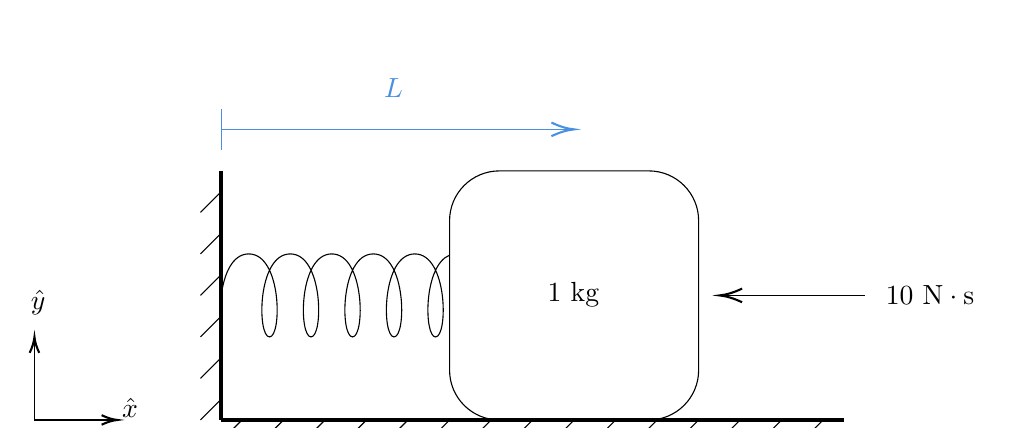
\begin{tikzpicture}[x=0.75pt,y=0.75pt,yscale=-1,xscale=1]
%uncomment if require: \path (0,300); %set diagram left start at 0, and has height of 300

%Rounded Rect [id:dp7768881234617668] 
\draw  [color={rgb, 255:red, 0; green, 0; blue, 0 }  ,draw opacity=1 ][fill={rgb, 255:red, 255; green, 255; blue, 255 }  ,fill opacity=1 ] (300,134) .. controls (300,120.75) and (310.75,110) .. (324,110) -- (396,110) .. controls (409.25,110) and (420,120.75) .. (420,134) -- (420,206) .. controls (420,219.25) and (409.25,230) .. (396,230) -- (324,230) .. controls (310.75,230) and (300,219.25) .. (300,206) -- cycle ;
%Straight Lines [id:da38466903419728604] 
\draw    (100,230) -- (100,192) ;
\draw [shift={(100,190)}, rotate = 90] [color={rgb, 255:red, 0; green, 0; blue, 0 }  ][line width=0.75]    (7.65,-2.3) .. controls (4.86,-0.97) and (2.31,-0.21) .. (0,0) .. controls (2.31,0.21) and (4.86,0.98) .. (7.65,2.3)   ;
%Straight Lines [id:da6153763296005214] 
\draw    (100,230) -- (138,230) ;
\draw [shift={(140,230)}, rotate = 180] [color={rgb, 255:red, 0; green, 0; blue, 0 }  ][line width=0.75]    (7.65,-2.3) .. controls (4.86,-0.97) and (2.31,-0.21) .. (0,0) .. controls (2.31,0.21) and (4.86,0.98) .. (7.65,2.3)   ;
%Shape: Spring [id:dp12565049584625476] 
\draw   (190,170) .. controls (191.25,160) and (195.25,150) .. (203.25,150) .. controls (219.25,150) and (219.25,190) .. (213.25,190) .. controls (207.25,190) and (207.25,150) .. (223.25,150) .. controls (239.25,150) and (239.25,190) .. (233.25,190) .. controls (227.25,190) and (227.25,150) .. (243.25,150) .. controls (259.25,150) and (259.25,190) .. (253.25,190) .. controls (247.25,190) and (247.25,150) .. (263.25,150) .. controls (279.25,150) and (279.25,190) .. (273.25,190) .. controls (267.25,190) and (267.25,150) .. (283.25,150) .. controls (299.25,150) and (299.25,190) .. (293.25,190) .. controls (287.69,190) and (287.28,155.62) .. (300,150.61) ;
%Straight Lines [id:da13717716944566494] 
\draw [line width=1.5]    (190,230) -- (490,230) ;
%Straight Lines [id:da08497529256460246] 
\draw [line width=1.5]    (190,110) -- (190,230) ;
%Straight Lines [id:da6451180344156043] 
\draw    (500,170) -- (432,170) ;
\draw [shift={(430,170)}, rotate = 360] [color={rgb, 255:red, 0; green, 0; blue, 0 }  ][line width=0.75]    (10.93,-3.29) .. controls (6.95,-1.4) and (3.31,-0.3) .. (0,0) .. controls (3.31,0.3) and (6.95,1.4) .. (10.93,3.29)   ;
%Straight Lines [id:da4484222824632662] 
\draw [color={rgb, 255:red, 74; green, 144; blue, 226 }  ,draw opacity=1 ]   (190,90) -- (358,90) ;
\draw [shift={(360,90)}, rotate = 180] [color={rgb, 255:red, 74; green, 144; blue, 226 }  ,draw opacity=1 ][line width=0.75]    (10.93,-3.29) .. controls (6.95,-1.4) and (3.31,-0.3) .. (0,0) .. controls (3.31,0.3) and (6.95,1.4) .. (10.93,3.29)   ;
%Straight Lines [id:da31603055366988764] 
\draw [color={rgb, 255:red, 74; green, 144; blue, 226 }  ,draw opacity=1 ]   (190,80) -- (190,100) ;
%Straight Lines [id:da3672906158385085] 
\draw    (190,240) -- (200,230) ;
%Straight Lines [id:da5740630070589421] 
\draw    (210,240) -- (220,230) ;
%Straight Lines [id:da7670589944898886] 
\draw    (230,240) -- (240,230) ;
%Straight Lines [id:da9623123722477054] 
\draw    (250,240) -- (260,230) ;
%Straight Lines [id:da09481544899973315] 
\draw    (270,240) -- (280,230) ;
%Straight Lines [id:da7618060743054186] 
\draw    (290,240) -- (300,230) ;
%Straight Lines [id:da06428960315401433] 
\draw    (310,240) -- (320,230) ;
%Straight Lines [id:da7732543318917602] 
\draw    (330,240) -- (340,230) ;
%Straight Lines [id:da7544212064888517] 
\draw    (350,240) -- (360,230) ;
%Straight Lines [id:da9699435924293961] 
\draw    (370,240) -- (380,230) ;
%Straight Lines [id:da4928357475624251] 
\draw    (390,240) -- (400,230) ;
%Straight Lines [id:da952354089719576] 
\draw    (410,240) -- (420,230) ;
%Straight Lines [id:da2820465635927757] 
\draw    (430,240) -- (440,230) ;
%Straight Lines [id:da7568084497678664] 
\draw    (450,240) -- (460,230) ;
%Straight Lines [id:da9121540373410668] 
\draw    (470,240) -- (480,230) ;
%Straight Lines [id:da17683266041429568] 
\draw    (180,130) -- (190,120) ;
%Straight Lines [id:da8134568638498193] 
\draw    (180,150) -- (190,140) ;
%Straight Lines [id:da9984593523585779] 
\draw    (180,170) -- (190,160) ;
%Straight Lines [id:da006829172139502071] 
\draw    (180,190) -- (190,180) ;
%Straight Lines [id:da45076310277705844] 
\draw    (180,210) -- (190,200) ;
%Straight Lines [id:da7407972176901751] 
\draw    (180,230) -- (190,220) ;

% Text Node
\draw (141,218.4) node [anchor=north west][inner sep=0.75pt]    {$\hat{x}$};
% Text Node
\draw (97,166.4) node [anchor=north west][inner sep=0.75pt]    {$\hat{y}$};
% Text Node
\draw (531.5,170) node    {$10\ \mathrm{N} \cdot \mathrm{s}$};
% Text Node
\draw (273,70) node  [color={rgb, 255:red, 74; green, 144; blue, 226 }  ,opacity=1 ]  {$L$};
% Text Node
\draw (346,162.4) node [anchor=north west][inner sep=0.75pt]    {$1\ \mathrm{kg}$};


\end{tikzpicture}


    \caption{Mass-Spring System Problem Set-Up}
    \label{fig:mass spring}
\end{figure}
\begin{enumerate}
    \item Consider the system to be frictionless. Derive the \glspl{eom} for the system in both of the component directions.
    \item Find the analytical solution of the system from the \gls{eom} you derived. Graph the solution.
    \item Numerically integrate the \glspl{eom} ascertain the position and velocity as a function of time. Graph the solution. How does it compare to the analytical solution? You may want to refer to Chapter \ref{sec:numerical integration schemes} for other numerical integration methods.
    \item Consider the system with some frictional force that is proportional to the velocity, with a proportionality constant of $c=1\mathrm{\frac{kg}{s}}$. This frictional force opposes the motion of the system. Repeat step c with this new system. How does the friction change the system?
\end{enumerate}
    \item After your escape from the frat house, you run into your friend, Buckminster, who is a big fan of circular-shaped objects. He asks you if you can model the orbit of a satellite to see if it looks anything like his geodesic domes. Not wanting to let him down, you write a MATLAB script to do so. You can assume the earth has a radius $R_\oplus=$6380 km and $\mu_\oplus=3.986\cdot10^5\, \frac{\mathrm{km^3}}{\mathrm{s^2}}$.
\begin{figure}[ht]
    \centering



\tikzset{every picture/.style={line width=0.75pt}} %set default line width to 0.75pt        

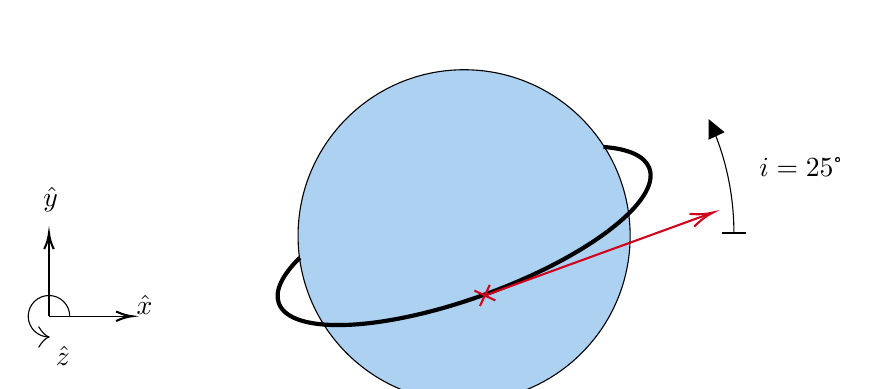
\begin{tikzpicture}[x=0.75pt,y=0.75pt,yscale=-1,xscale=1]
%uncomment if require: \path (0,300); %set diagram left start at 0, and has height of 300

%Shape: Circle [id:dp16691195552333382] 
\draw  [color={rgb, 255:red, 0; green, 0; blue, 0 }  ,draw opacity=1 ][fill={rgb, 255:red, 173; green, 209; blue, 241 }  ,fill opacity=1 ] (260,161.23) .. controls (260,117.05) and (295.82,81.23) .. (340,81.23) .. controls (384.18,81.23) and (420,117.05) .. (420,161.23) .. controls (420,205.42) and (384.18,241.23) .. (340,241.23) .. controls (295.82,241.23) and (260,205.42) .. (260,161.23) -- cycle ;
%Straight Lines [id:da08799392003464845] 
\draw    (140,200) -- (140,162) ;
\draw [shift={(140,160)}, rotate = 90] [color={rgb, 255:red, 0; green, 0; blue, 0 }  ][line width=0.75]    (7.65,-2.3) .. controls (4.86,-0.97) and (2.31,-0.21) .. (0,0) .. controls (2.31,0.21) and (4.86,0.98) .. (7.65,2.3)   ;
%Straight Lines [id:da16946831015851427] 
\draw    (140,200) -- (178,200) ;
\draw [shift={(180,200)}, rotate = 180] [color={rgb, 255:red, 0; green, 0; blue, 0 }  ][line width=0.75]    (7.65,-2.3) .. controls (4.86,-0.97) and (2.31,-0.21) .. (0,0) .. controls (2.31,0.21) and (4.86,0.98) .. (7.65,2.3)   ;
%Shape: Arc [id:dp2632274214469099] 
\draw  [draw opacity=0] (140,210) .. controls (140,210) and (140,210) .. (140,210) .. controls (140,210) and (140,210) .. (140,210) .. controls (134.48,210) and (130,205.52) .. (130,200) .. controls (130,194.48) and (134.48,190) .. (140,190) .. controls (145.52,190) and (150,194.48) .. (150,200) -- (140,200) -- cycle ; \draw   (140,210) .. controls (140,210) and (140,210) .. (140,210) .. controls (140,210) and (140,210) .. (140,210) .. controls (134.48,210) and (130,205.52) .. (130,200) .. controls (130,194.48) and (134.48,190) .. (140,190) .. controls (145.52,190) and (150,194.48) .. (150,200) ;  
\draw   (135,205) .. controls (136.67,207.78) and (138.33,209.44) .. (140,210) .. controls (138.33,210.56) and (136.67,212.22) .. (135,215) ;
%Shape: Arc [id:dp9820699747427737] 
\draw  [draw opacity=0] (457.85,105.05) .. controls (465.65,121.74) and (470,140.36) .. (470,160) -- (340,160) -- cycle ; \draw    (459.1,107.82) .. controls (466.11,123.79) and (470,141.44) .. (470,160) ; \draw [shift={(470,160)}, rotate = 270] [color={rgb, 255:red, 0; green, 0; blue, 0 }  ][line width=0.75]    (0,5.59) -- (0,-5.59)   ; \draw [shift={(457.85,105.05)}, rotate = 64.96] [fill={rgb, 255:red, 0; green, 0; blue, 0 }  ][line width=0.08]  [draw opacity=0] (8.93,-4.29) -- (0,0) -- (8.93,4.29) -- cycle    ;
%Shape: Arc [id:dp4819431408488013] 
\draw  [draw opacity=0][line width=1.5]  (407.17,118.44) .. controls (419.05,119.31) and (427.08,122.71) .. (429.27,128.74) .. controls (434.94,144.31) and (399.56,171.48) .. (350.26,189.42) .. controls (300.96,207.37) and (256.4,209.29) .. (250.73,193.73) .. controls (248.55,187.74) and (252.44,180.03) .. (260.87,171.79) -- (340,161.23) -- cycle ; \draw  [line width=1.5]  (407.17,118.44) .. controls (419.05,119.31) and (427.08,122.71) .. (429.27,128.74) .. controls (434.94,144.31) and (399.56,171.48) .. (350.26,189.42) .. controls (300.96,207.37) and (256.4,209.29) .. (250.73,193.73) .. controls (248.55,187.74) and (252.44,180.03) .. (260.87,171.79) ;  
%Straight Lines [id:da7892814012335462] 
\draw [color={rgb, 255:red, 208; green, 2; blue, 27 }  ,draw opacity=1 ][line width=0.75]    (350,190) -- (458.12,150.68) ;
\draw [shift={(460,150)}, rotate = 160.02] [color={rgb, 255:red, 208; green, 2; blue, 27 }  ,draw opacity=1 ][line width=0.75]    (10.93,-3.29) .. controls (6.95,-1.4) and (3.31,-0.3) .. (0,0) .. controls (3.31,0.3) and (6.95,1.4) .. (10.93,3.29)   ;
\draw [shift={(350,190)}, rotate = 25.02] [color={rgb, 255:red, 208; green, 2; blue, 27 }  ,draw opacity=1 ][line width=0.75]    (-5.59,0) -- (5.59,0)(0,5.59) -- (0,-5.59)   ;

% Text Node
\draw (181,188.4) node [anchor=north west][inner sep=0.75pt]    {$\hat{x}$};
% Text Node
\draw (142,213.4) node [anchor=north west][inner sep=0.75pt]    {$\hat{z}$};
% Text Node
\draw (481,122.4) node [anchor=north west][inner sep=0.75pt]    {$i=25\degree $};
% Text Node
\draw (136,136.4) node [anchor=north west][inner sep=0.75pt]    {$\hat{y}$};

\end{tikzpicture}

    \caption{Satellite in Orbit Problem Set-Up}
    \label{fig:orbit}
\end{figure}
\begin{enumerate}
    \item Assuming 3-\gls{dof}, derive the \gls{eom} for the satellite motion assuming that gravity is the only force acting on the satellite and the earth is a point mass. \textit{Hint: You may want to use a different coordinate system.}
    \item You find a satellite in orbit with a height of 400 km. You also measure the inclination of the orbit as it passes overhead as $25\degree$. Assuming a circular orbit, what is the magnitude of the velocity and the component velocities in $\hat{x}$ and $\hat{y}$ as it passes overhead?
\end{enumerate}
    \item  NASA, inspired by your expert analysis of the orbit, asks you to help analyze the rotational dynamics of the Explorer 1 satellite for your job interview. The satellite can be modeled approximately as a cylinder with a length of 2 m and a diameter of 16 cm. Assume the mass is 16kg with a uniform mass distribution.
\begin{figure}[ht]
    \centering
 
\tikzset{every picture/.style={line width=0.75pt}} %set default line width to 0.75pt        

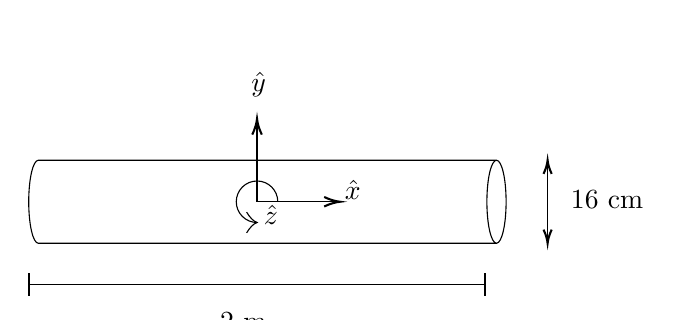
\begin{tikzpicture}[x=0.75pt,y=0.75pt,yscale=-1,xscale=1]
%uncomment if require: \path (0,300); %set diagram left start at 0, and has height of 300

%Shape: Can [id:dp21172872656172192] 
\draw   (435.38,171) -- (214.63,171) .. controls (212.07,171) and (210,162.05) .. (210,151) .. controls (210,139.95) and (212.07,131) .. (214.63,131) -- (435.38,131) .. controls (437.93,131) and (440,139.95) .. (440,151) .. controls (440,162.05) and (437.93,171) .. (435.38,171) .. controls (432.82,171) and (430.75,162.05) .. (430.75,151) .. controls (430.75,139.95) and (432.82,131) .. (435.38,131) ;
%Straight Lines [id:da41388689366433795] 
\draw    (320,151) -- (320,113) ;
\draw [shift={(320,111)}, rotate = 90] [color={rgb, 255:red, 0; green, 0; blue, 0 }  ][line width=0.75]    (7.65,-2.3) .. controls (4.86,-0.97) and (2.31,-0.21) .. (0,0) .. controls (2.31,0.21) and (4.86,0.98) .. (7.65,2.3)   ;
%Straight Lines [id:da6701135215445572] 
\draw    (320,151) -- (358,151) ;
\draw [shift={(360,151)}, rotate = 180] [color={rgb, 255:red, 0; green, 0; blue, 0 }  ][line width=0.75]    (7.65,-2.3) .. controls (4.86,-0.97) and (2.31,-0.21) .. (0,0) .. controls (2.31,0.21) and (4.86,0.98) .. (7.65,2.3)   ;
%Shape: Arc [id:dp6670514917911996] 
\draw  [draw opacity=0] (320,161) .. controls (320,161) and (320,161) .. (320,161) .. controls (320,161) and (320,161) .. (320,161) .. controls (314.48,161) and (310,156.52) .. (310,151) .. controls (310,145.48) and (314.48,141) .. (320,141) .. controls (325.52,141) and (330,145.48) .. (330,151) -- (320,151) -- cycle ; \draw   (320,161) .. controls (320,161) and (320,161) .. (320,161) .. controls (320,161) and (320,161) .. (320,161) .. controls (314.48,161) and (310,156.52) .. (310,151) .. controls (310,145.48) and (314.48,141) .. (320,141) .. controls (325.52,141) and (330,145.48) .. (330,151) ;  
\draw   (315,156) .. controls (316.67,158.78) and (318.33,160.44) .. (320,161) .. controls (318.33,161.56) and (316.67,163.22) .. (315,166) ;
%Straight Lines [id:da9894971015882463] 
\draw    (210,191) -- (430,191) ;
\draw [shift={(430,191)}, rotate = 180] [color={rgb, 255:red, 0; green, 0; blue, 0 }  ][line width=0.75]    (0,5.59) -- (0,-5.59)   ;
\draw [shift={(210,191)}, rotate = 180] [color={rgb, 255:red, 0; green, 0; blue, 0 }  ][line width=0.75]    (0,5.59) -- (0,-5.59)   ;
%Straight Lines [id:da08378461172235874] 
\draw    (460,169) -- (460,133) ;
\draw [shift={(460,131)}, rotate = 90] [color={rgb, 255:red, 0; green, 0; blue, 0 }  ][line width=0.75]    (6.56,-1.97) .. controls (4.17,-0.84) and (1.99,-0.18) .. (0,0) .. controls (1.99,0.18) and (4.17,0.84) .. (6.56,1.97)   ;
\draw [shift={(460,171)}, rotate = 270] [color={rgb, 255:red, 0; green, 0; blue, 0 }  ][line width=0.75]    (6.56,-1.97) .. controls (4.17,-0.84) and (1.99,-0.18) .. (0,0) .. controls (1.99,0.18) and (4.17,0.84) .. (6.56,1.97)   ;

% Text Node
\draw (361,139.4) node [anchor=north west][inner sep=0.75pt]    {$\hat{x}$};
% Text Node
\draw (322,151.4) node [anchor=north west][inner sep=0.75pt]    {$\hat{z}$};
% Text Node
\draw (316,87.4) node [anchor=north west][inner sep=0.75pt]    {$\hat{y}$};
% Text Node
\draw (301,203.4) node [anchor=north west][inner sep=0.75pt]    {$2\ \mathrm{m}$};
% Text Node
\draw (470,144.4) node [anchor=north west][inner sep=0.75pt]    {$16\ \mathrm{cm}$};


\end{tikzpicture}

    \caption{Explorer 1 Satellite}
    \label{fig:explorer 1}
\end{figure}
\begin{enumerate}
    \item Calculate the moment of inertia for the Explorer 1 in the body frame along each of the axes. \textit{Hint: You may benefit from a change in coordinate system.}
    \item NASA wants to spin-stabilize the satellite with a final rotation rate of $2\pi \ \mathrm{rad/s}$. Calculate the total impulse needed by small spin motors mounted on the circumference of the satellite to achieve this rotation rate. You may assume that this impulse is provided by two motors, so that they act as a force couple.
    \item After the spin stabilization maneuver is done to inject the satellite into its final orbit, NASA wants to slow the satellite down by using a yo-yo de-spin. Suppose the satellite has two weights, each of mass 0.5 kg, that are tied to massless strings on the satellite. Assuming that these weights can be approximated as point masses, find the necessary length of the strings so that the final rotation rate of the satellite is $5 \ \mathrm{rpm}$.
\end{enumerate}
\end{enumerate}
\chapter{Energy Methods of Mechanics}\label{sec:energy methods}
\begin{chapquote}{Joseph Fourier}
    ''Mathematics compares the most diverse phenomena and discovers the secret analogies that unite them.''
\end{chapquote}

Energy methods of mechanics employ the concepts of the energy of a system to solve a problem in mechanics. This is in contrast to the Newtonian method, which considers the forces of a system. The good news is that both will result in the same answer (see proof in \ref{equiv newt and lang}). However, having both in your set of tools as an engineer can prove especially useful.

To grasp energy methods, it is best to have an intuition for Newtonian dynamics first. A thorough reading of Chapter \ref{sec: Newtonian Dynamics} and other sources will help prepare the reader for this section.

There are two main types of energy mechanics, referred to as Hamiltonian and Lagrangian Mechanics. In this chapter, we will mostly focus on the Lagrangian version of these mechanics. Hamiltonian mechanics are arguably more fundamental, but will only be briefly discussed.

\newglossaryentry{symplectic int}
{
    name=symplectic integrator,
    first = {\textit{symplectic integrator}},
    description={A class of numerical integration schemes that are energy preserving because they preserve certain geometric properties of a differential equation}
}

Although the Hamiltonian and Lagrangian are not directly used in the case of our 6-\gls{dof}, they are fundamental to other areas of mechanics and make derivations far simpler in many cases. The Hamiltonian and Lagrangian descriptions of mechanics are more often taught to physics students rather than engineers, but we feel that they deserve inclusion among the topics presented here. When we discuss numerical integration, we can use \glspl{symplectic int} when our problem has a Hamiltonian description. This will be further discussed in Section \ref{sec:other numerical ints}. You may find that certain \gls{eom} derivations, such as the spinning top and problems in orbital mechanics are more easily accomplished with energy methods.

Another reason to motivate these systems is that these energy methods are rotationally invariant because energy methods can employ a generalized coordinate system. These generalized coordinates are very powerful and allow us to describe a huge variety of systems. We will see this later in some examples.

A brief overview of the differences between the two schemes of \gls{eom} derivation is shown in Figure \ref{fig:newt v lang}

\begin{figure}[ht]
    \centering
    
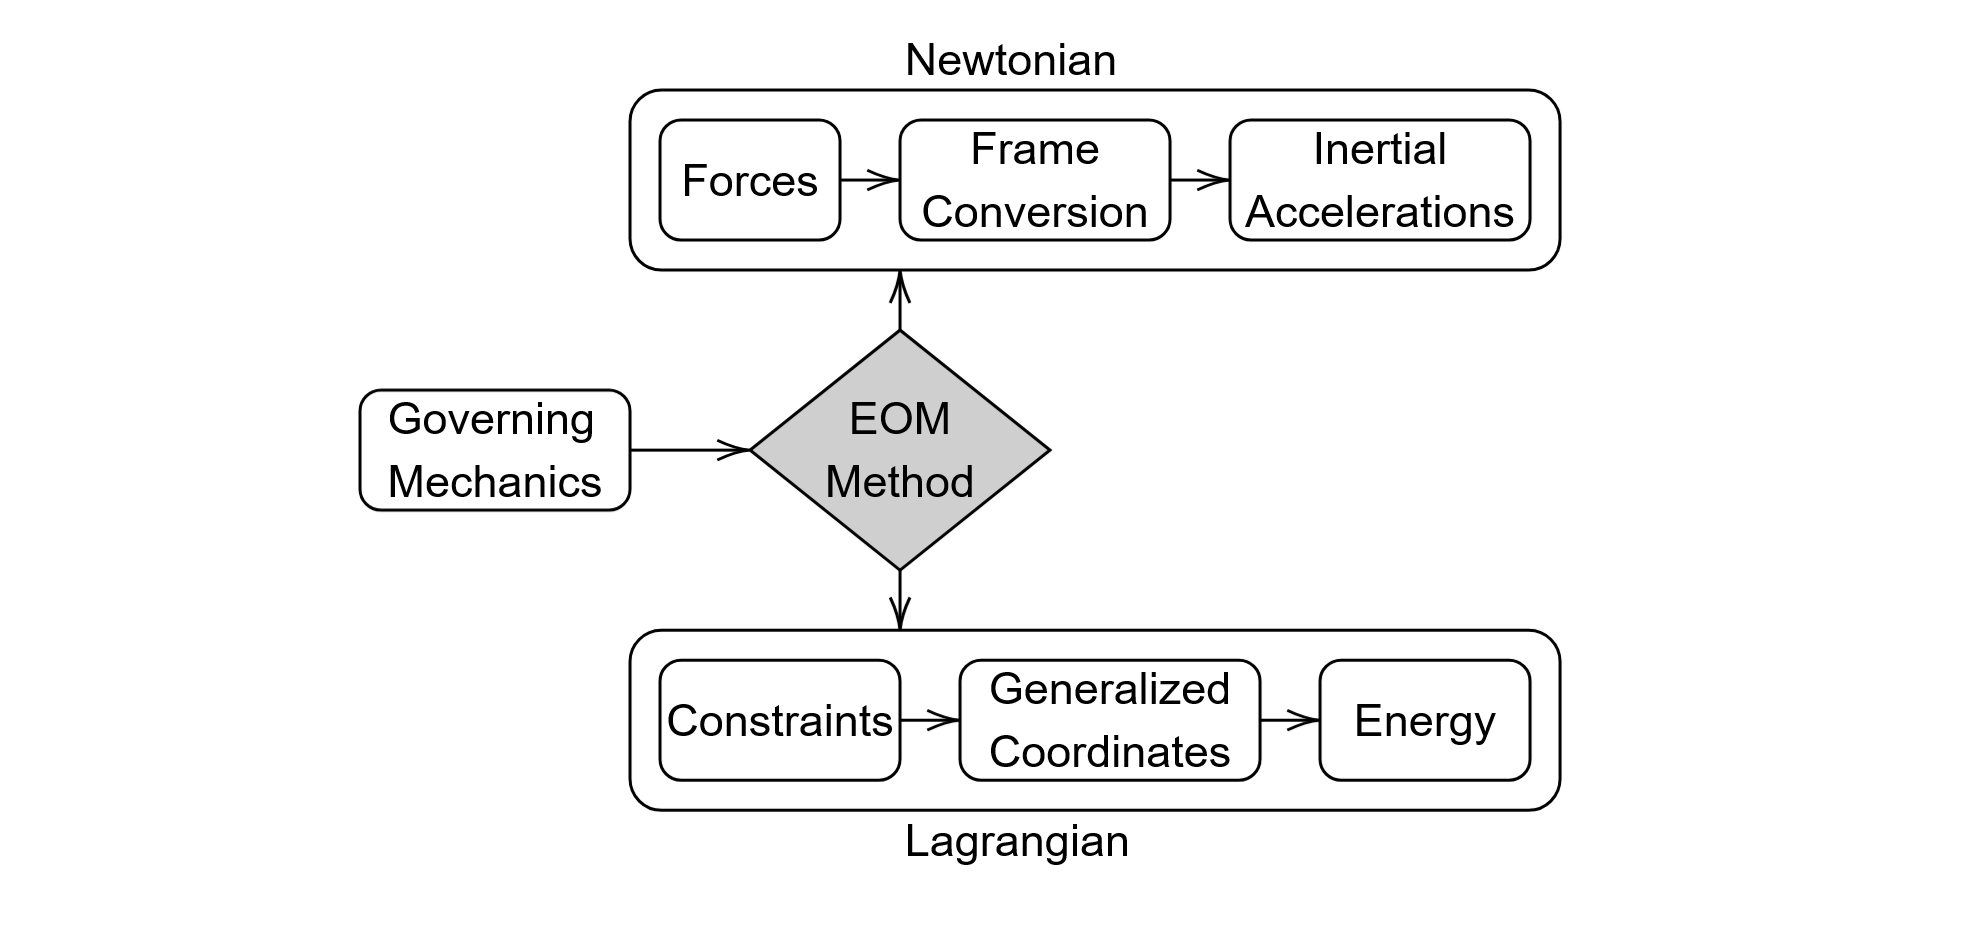
\includegraphics[width=\linewidth]{Images/diagram-20250322.png}

    \caption{Newtonian vs. Lagrangian Mechanics Approach}
    \label{fig:newt v lang}
\end{figure}

\section{Calculus of Variations}

The calculus of variations underpins the ideas of Lagrangian and Hamiltonian mechanics, so it is important to understand the principles behind it before moving on to the actual mechanics. In analogy to how single variable calculus is fundamental to Newtonian mechanics, the calculus of variations is fundamental to energy mechanics.

\newglossaryentry{geodesic}
{
    name=geodesic,
    first = {\textit{geodesic}},
    description={The shortest path between two points in an arbitrarily curved space}
}

The fundamental idea of the calculus of variations is simple. We want to find the maximums and minimums of some quantity in our problem. Why? In physics, we often see that quantities are minimized or maximized for some reason. For example, a soap surface will minimize its surface area, or a beam of photons will follow a \gls{geodesic} of spacetime. Light will also refract through surfaces to minimize time as seen in Snell's Law. 

Because so many physical phenomena are governed by this behavior to minimize certain quantities, Hamilton (the same mathematical hero we will see later with attitude dynamics), decided to formulate a mathematical description of this.

\newglossaryentry{functional}
{
    name=functional,
    first = {\textit{functional}},
    description={A quantity that maps a function onto the real number line. Often,  this is called a 'function of a function'}
}

Before we get to Hamilton's formulation, we need to understand what the calculus of variations is trying to do. To find a minima means that naturally, we should look for the extrema of some quantity. We call this quantity a \gls{functional}, which we define as:
\begin{equation}\label{eq:functional}
    J=\int_{x_1}^{x_2}f\left[y(x),y'(x);x\right]{dx}
\end{equation}
The \gls{functional}, $J$, is a quantity which maps a function onto the real number line. This means that it takes the function as an input and outputs a single real number. We are attempting to find an input function, $y(x)$, that yields an extrema of $J$. 

\newglossaryentry{neigh func}
{
    name=neighborhood function,
    first = {\textit{neighborhood function}},
    description={A small function added to another function in the calculus of variations. Analogous to a differential element in single variate calculus}
}

To be precise about this definition of an extrema - we are attempting to find a function $y(x)$ such that any other function added to $y(x)$, no matter how close it is to $y(x)$, must change the value of $J$ such that it is no longer an extrema. By convention, this other function added to $y(x)$ is called the \gls{neigh func}, and is denoted $\eta(x)$.

We can compactly write this $y(x)+\eta(x)$ as $y(\varepsilon,x)$. We define the condition $y(0,x)\equiv y(x)$, where $y(x)$ is the function that gives the extrema of $J$. So, we can write $y(\varepsilon,x)$ as
\begin{equation}\label{eq:y epsilon}
    y(\varepsilon,x)=y(0,x)+\varepsilon\eta(x)
\end{equation}
The important restriction that we impose on $\eta(x)$ is that it must vanish at the endpoints, $x_1$ and $x_2$. This will prove important later so we can apply integration rules on our function. We also want a continuous first derivative so that $y'(\varepsilon,x)$ can be defined as
\begin{equation}\label{eq:y prime epsilon}
    y'(\varepsilon,x)=\frac{dy(0,x)}{dx}+\varepsilon\frac{d\eta}{dx}
\end{equation}

Using this definition of the \gls{neigh func}, we can rewrite \eqref{eq:functional} as
\begin{equation}\label{eq:neighborhood functional}
    J(\varepsilon)=\int_{x_1}^{x_2}f\left[y(\varepsilon,x),y'(\varepsilon,x);x\right]{dx}
\end{equation}
So, with this redefined version of the function, we can finally find the extrema using the familiar calculus rule, setting the derivative equal to zero. We also evaluate at zero since this is where we defined the extrema to exist:
\begin{equation}
    \left.\frac{\partial J(\varepsilon)}{\partial\varepsilon}\right\vert_{\varepsilon=0}=0
\end{equation}
Applying this to \eqref{eq:functional}, we arrive at
\begin{equation}\label{eq:neighborhood functional diff}
    \frac{\partial J(\varepsilon)}{\partial\varepsilon}= \frac{\partial}{\partial\varepsilon}\int_{x_1}^{x_2}f\left[y(0,x),y'(0,x);x\right]{dx}
\end{equation}
The $\varepsilon$ terms drop out from the RHS from the evaluation of $\varepsilon=0$. Applying the Leibniz Integral Rule, the partial derivative can be moved inside the RHS integral:
\begin{equation}
    \frac{\partial J(\varepsilon)}{\partial\varepsilon}= \int_{x_1}^{x_2}\frac{\partial}{\partial\varepsilon}f\left[y(x),y'(x);x\right]{dx}
\end{equation}
Applying the rules of implicit integration on the integrand, we get:
\begin{equation}\label{eq:diff functional}
    \frac{\partial J(\varepsilon)}{\partial\varepsilon}= \int_{x_1}^{x_2}f\left(\frac{\partial f}{\partial y}\frac{\partial y}{\partial\varepsilon}+\frac{\partial f}{\partial y'}\frac{\partial y'}{\partial\varepsilon}\right){dx}
\end{equation}
Note that we still must take the partial derivative with respect to $\varepsilon$ on the RHS, even though we have plugged in 0 for $\varepsilon$.

Next, we can find expressions for $\frac{\partial y}{\partial \varepsilon}$ and $\frac{\partial y'}{\partial \varepsilon}$. This is done with the expressions \eqref{eq:y epsilon} and \eqref{eq:y prime epsilon}. Starting with the first, we differentiate \eqref{eq:y epsilon} with respect to $\varepsilon$:
\begin{equation}\label{eq:y diff epsilon}
    \frac{\partial}{\partial \varepsilon}y(\varepsilon,x)=\frac{\partial}{\partial \varepsilon}\left[y(0,x)+\varepsilon\eta(x)\right]
\end{equation}
Here, $y(0,x)$ is independent of $\varepsilon$ since we define it to occur at value $\varepsilon=0$. So this leaves us with
\begin{equation}\label{eq:diff y diff epsilon}
     \frac{\partial y}{\partial \varepsilon}= \eta(x)
\end{equation}
Doing the same for \eqref{eq:y diff epsilon}, we arrive at
\begin{equation}\label{diff y' diff epsilon}
     \frac{\partial y'}{\partial \varepsilon}= \frac{\partial \eta}{\partial x}
\end{equation}
Finally, plugging these back into the original expression for \eqref{eq:diff functional}, we get the expression
\begin{equation}\label{eq:diff functional subs}
    \frac{\partial J(\varepsilon)}{\partial\varepsilon}= \int_{x_1}^{x_2}\left(\frac{\partial f}{\partial y}\eta(x)+\frac{\partial f}{\partial y'}\frac{\partial \eta}{\partial x}\right){dx}
\end{equation}
Finally, performing some integration by parts, we arrive at the final integral expression of the maximum:
\begin{equation}\label{eq:diff functional final}
    \frac{\partial J(\varepsilon)}{\partial\varepsilon}= \int_{x_1}^{x_2}\left(\frac{\partial f}{\partial y}-\frac{d}{dx}\frac{\partial f}{\partial y'}\right)\eta(x){dx}
\end{equation}
Since we are evaluating the maximum, $\frac{\partial J(\varepsilon)}{\partial\varepsilon}$ evaluates to 0. Since $\eta(x)$ is an arbitrary function, the only way to guarantee an equality is to ensure that the part of the integrand in parenthesis is 0.

\newglossaryentry{Euler Equation}
{
    name=Euler's equation,
    first = {\textit{Euler's equation}},
    description={The fundemental equation in the calculus of variations describing the maximum or minimum conditions of a functional},
    see={functional}
}

This gives us the fundamental equation of the calculus of variations, called \gls{Euler Equation}:
\begin{equation}\label{eq: Euler's Diff eq}
    \frac{\partial f}{\partial y}-\frac{d}{dx}\frac{\partial f}{\partial y'}=0
\end{equation}
\subsection{Delta Notation}
In later sections, it is useful to have a shorthand for these partial derivative quantities. For a quantity $\chi$, the variation, $\delta$ is given as:
$$\delta\equiv\frac{\partial\chi}{\partial \varepsilon}d\varepsilon$$Using this notation, we can rewrite \eqref{eq:diff functional final} after some algebraic manipulation as:
\begin{equation}
    \delta J= \int_{x_1}^{x_2}\left(\frac{\partial f}{\partial y}-\frac{d}{dx}\frac{\partial f}{\partial y'}\right)\delta y{dx}
\end{equation}
And thus, \eqref{eq: Euler's Diff eq} can be written concisely as:
\begin{equation}
    \color{blue}\boxed{\color{black}\delta J=0}
\end{equation}
This is a very general and far reaching conclusion that can be applied to many systems. For our use cases in dynamics, we have more useful forms of this equation which will be explored in the following section.

\section{Hamilton's Principle}

Following directly from the ideas of the calculus of variations, Hamilton (alongside many other mathematicians) wanted to apply this to physical systems. Hamilton's Principle is as follows:
\begin{theorem}[Hamilton's Principle]
A system which may travel from one point to another within a specific time interval, the path that is followed is the path which minimizes the time integral of the difference between the kinetic and potential energies.
$$\delta \int_{t_1}^{t_2}{T-U}{dt}=0$$
\end{theorem}
\newglossaryentry{Lagrangian}
{
    name=Lagrangian,
    first = {\textit{Lagrangian}},
    description={A description of the energy of a system given by $L\equiv T-U$. Denoted with the letter $L$}
}

The quantity $T-U$, the kinetic energy minus the potential energy, is a quantity called the \gls{Lagrangian}, denoted $L$. 
\begin{equation}
    L\equiv T-U
\end{equation}

\newglossaryentry{action}
{
    name=action,
    first = {\textit{action}},
    description={The time integral of energy is known as the action, which is often denoted $S$}
}

\newglossaryentry{princ of least action}
{
    name=principle of least action,
    first = {\textit{principle of least action}},
    description={A form of Hamilton's Principle that states that the action of a system should be minimized in a physical mechanical system.},
    see={action}
}

The time integral of the \gls{Lagrangian} is the \gls{action}, denoted $S$. This is often why Hamilton's Principle is also called the \gls{princ of least action}. 

\begin{equation}
    S=\int_{t_1}^{t_2}{L}{dt}
\end{equation}
So, our action takes the form of the \gls{functional} from the calculus of variations. From Hamilton's principle, this \gls{functional}, the action, must be minimized. So, we often see the compact form of Hamilton's Principle as:
$$\delta S=0$$

\newglossaryentry{euler lagrange}
{
    name=Euler-Lagrange Equation,
    first = {\textit{Euler-Lagrange Equation}},
    description={The fundemental equations describing the solutions that give the extrema of the action in a Lagrangian system},
    see={action, Lagrangian}
}

Expressed using Euler's differential equation, \eqref{eq: Euler's Diff eq}, we get the \glspl{euler lagrange}:
\begin{gather}\label{eq: Euler-Lagrange}
    \color{blue}\boxed{\color{black}\frac{\partial L}{\partial x_i}-\frac{d}{dt}\frac{\partial L}{\partial \dot{x}_i}=0}\\ \mathrm{\color{blue}Euler-Lagrange \ Equations}
\end{gather}
Before we look into some examples of how to utilize these equations in practice, we should consider in what situations these will be better than the Newtonian methods.

\newglossaryentry{conservative}
{
    name=conservative,
    first = {\textit{conservative}},
    description={A system or potential which is independent of the path. A closed integral in a conservative field is 0}
}

We note that in this chapter, we will only consider potential functions which are \gls{conservative}, or path independent. This does mean that frictional forces and aerodynamics are not modeled with the \gls{Lagrangian} we describe here (although they can be with the utilization of Rayleigh's dissipation function and other techniques, such as those discussed in \cite{rabei_hamiltonian_2004}). This is the reason we do not directly use these equations in the 6-DoF.\footnote{However, much of the rotational dynamics we describe can be represented equivalently using the \gls{Lagrangian} approach, so we do use these equations in a roundabout manner.}

So, for systems that are non-conservative, it is best to stick with the Newtonian method of mechanics, as we do for our 6-DoF. However, for those that are frictionless, the methods described here will work well. While it may seem that frictionless systems are very idealistic, we do see systems that can be approximated as frictionless quite often! Orbits, of course, are one case where this is especially true. For many other systems, such as a spinning top or other rotating bodies, we can often ignore the small amount of friction and arrive at analytical solutions without much hassle using the \gls{Lagrangian}. These methods also become extraordinarily important for our derivations of rotational equations.

With that noted, let us use the \gls{Lagrangian} in a few examples to see how it can turn some complex Newtonian systems into fairly trivial problems.
\subsection{Mass-Spring System}
As a very basic first system, we will consider a mass spring system as shown in Figure \ref{fig:mass spring lagrange}. We consider the length $x$ to be referenced from the rest length of the spring.
\begin{figure}[ht]

\centering

\tikzset{every picture/.style={line width=0.75pt}} %set default line width to 0.75pt        

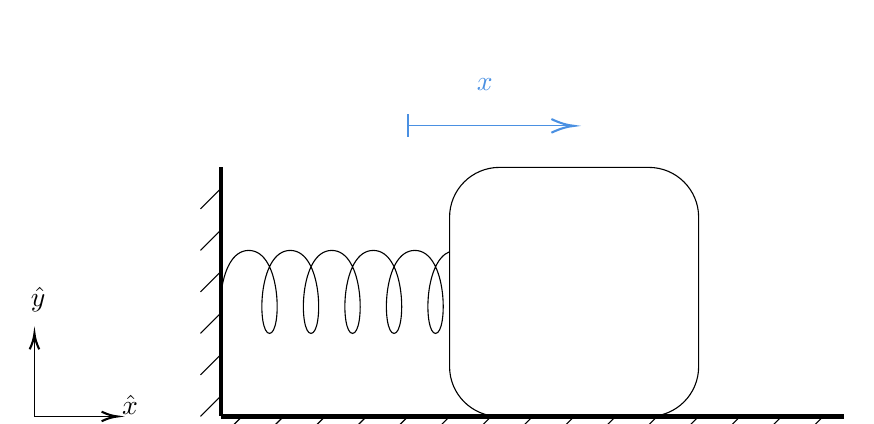
\begin{tikzpicture}[x=0.75pt,y=0.75pt,yscale=-1,xscale=1]
%uncomment if require: \path (0,300); %set diagram left start at 0, and has height of 300

%Rounded Rect [id:dp34438430167397516] 
\draw  [color={rgb, 255:red, 0; green, 0; blue, 0 }  ,draw opacity=1 ][fill={rgb, 255:red, 255; green, 255; blue, 255 }  ,fill opacity=1 ] (310,154) .. controls (310,140.75) and (320.75,130) .. (334,130) -- (406,130) .. controls (419.25,130) and (430,140.75) .. (430,154) -- (430,226) .. controls (430,239.25) and (419.25,250) .. (406,250) -- (334,250) .. controls (320.75,250) and (310,239.25) .. (310,226) -- cycle ;
%Straight Lines [id:da2744613466135113] 
\draw    (110,250) -- (110,212) ;
\draw [shift={(110,210)}, rotate = 90] [color={rgb, 255:red, 0; green, 0; blue, 0 }  ][line width=0.75]    (7.65,-2.3) .. controls (4.86,-0.97) and (2.31,-0.21) .. (0,0) .. controls (2.31,0.21) and (4.86,0.98) .. (7.65,2.3)   ;
%Straight Lines [id:da08431663295207847] 
\draw    (110,250) -- (148,250) ;
\draw [shift={(150,250)}, rotate = 180] [color={rgb, 255:red, 0; green, 0; blue, 0 }  ][line width=0.75]    (7.65,-2.3) .. controls (4.86,-0.97) and (2.31,-0.21) .. (0,0) .. controls (2.31,0.21) and (4.86,0.98) .. (7.65,2.3)   ;
%Shape: Spring [id:dp2050444045141704] 
\draw   (200,190) .. controls (201.25,180) and (205.25,170) .. (213.25,170) .. controls (229.25,170) and (229.25,210) .. (223.25,210) .. controls (217.25,210) and (217.25,170) .. (233.25,170) .. controls (249.25,170) and (249.25,210) .. (243.25,210) .. controls (237.25,210) and (237.25,170) .. (253.25,170) .. controls (269.25,170) and (269.25,210) .. (263.25,210) .. controls (257.25,210) and (257.25,170) .. (273.25,170) .. controls (289.25,170) and (289.25,210) .. (283.25,210) .. controls (277.25,210) and (277.25,170) .. (293.25,170) .. controls (309.25,170) and (309.25,210) .. (303.25,210) .. controls (297.69,210) and (297.28,175.62) .. (310,170.61) ;
%Straight Lines [id:da8109677911849542] 
\draw [line width=1.5]    (200,250) -- (500,250) ;
%Straight Lines [id:da9738860715008741] 
\draw [line width=1.5]    (200,130) -- (200,250) ;
%Straight Lines [id:da8479892294914445] 
\draw [color={rgb, 255:red, 74; green, 144; blue, 226 }  ,draw opacity=1 ]   (290,110) -- (368,110) ;
\draw [shift={(370,110)}, rotate = 180] [color={rgb, 255:red, 74; green, 144; blue, 226 }  ,draw opacity=1 ][line width=0.75]    (10.93,-3.29) .. controls (6.95,-1.4) and (3.31,-0.3) .. (0,0) .. controls (3.31,0.3) and (6.95,1.4) .. (10.93,3.29)   ;
\draw [shift={(290,110)}, rotate = 180] [color={rgb, 255:red, 74; green, 144; blue, 226 }  ,draw opacity=1 ][line width=0.75]    (0,5.59) -- (0,-5.59)   ;
%Straight Lines [id:da38778280879589844] 
\draw    (200,260) -- (210,250) ;
%Straight Lines [id:da13716831040628819] 
\draw    (220,260) -- (230,250) ;
%Straight Lines [id:da5435450145291132] 
\draw    (240,260) -- (250,250) ;
%Straight Lines [id:da6012450156738026] 
\draw    (260,260) -- (270,250) ;
%Straight Lines [id:da006204164316379712] 
\draw    (280,260) -- (290,250) ;
%Straight Lines [id:da6672054023307342] 
\draw    (300,260) -- (310,250) ;
%Straight Lines [id:da05532576658672206] 
\draw    (320,260) -- (330,250) ;
%Straight Lines [id:da713074642825677] 
\draw    (340,260) -- (350,250) ;
%Straight Lines [id:da054951797337481234] 
\draw    (360,260) -- (370,250) ;
%Straight Lines [id:da44290965384713543] 
\draw    (380,260) -- (390,250) ;
%Straight Lines [id:da1554621606788551] 
\draw    (400,260) -- (410,250) ;
%Straight Lines [id:da18496092525096441] 
\draw    (420,260) -- (430,250) ;
%Straight Lines [id:da9097830383289192] 
\draw    (440,260) -- (450,250) ;
%Straight Lines [id:da2668563479968923] 
\draw    (460,260) -- (470,250) ;
%Straight Lines [id:da6488797889553993] 
\draw    (480,260) -- (490,250) ;
%Straight Lines [id:da8070575578091496] 
\draw    (190,150) -- (200,140) ;
%Straight Lines [id:da3401604231163561] 
\draw    (190,170) -- (200,160) ;
%Straight Lines [id:da12031548793524682] 
\draw    (190,190) -- (200,180) ;
%Straight Lines [id:da3325006766252374] 
\draw    (190,210) -- (200,200) ;
%Straight Lines [id:da6789154128761035] 
\draw    (190,230) -- (200,220) ;
%Straight Lines [id:da23421921174832838] 
\draw    (190,250) -- (200,240) ;

% Text Node
\draw (151,238.4) node [anchor=north west][inner sep=0.75pt]    {$\hat{x}$};
% Text Node
\draw (107,186.4) node [anchor=north west][inner sep=0.75pt]    {$\hat{y}$};
% Text Node
\draw (327,90) node  [color={rgb, 255:red, 74; green, 144; blue, 226 }  ,opacity=1 ]  {$x$};

\end{tikzpicture}

    \caption{Mass-Spring System for Lagrangian}
    \label{fig:mass spring lagrange}
\end{figure}

We know the analytical form of the \gls{eom} from Newtonian Dynamics:
$$m\ddot{x}+kx=0$$
So, in essence, we are using the \gls{Lagrangian} \textit{a posteriori} to match this solution.

First, we will find the \gls{Lagrangian} of the system. The kinetic energy of the particle is given by the linear translation only (there is no rotational motion for a point particle), so we have $T=\frac{1}{2}m\dot{x}^2$. The potential energy is the energy of the spring, given as $U=\frac{1}{2}kx^2$. So, the \gls{Lagrangian} is:
$$L=\frac{1}{2}m\dot{x}^2-\frac{1}{2}kx^2$$
Now, applying \eqref{eq: Euler-Lagrange} in the $\hat{x}$-direction, as this is the only degree of freedom:
$$\frac{\partial L}{\partial x}-\frac{d}{dt}\frac{\partial L}{\partial \dot{x}}=0$$
Taking each term individually,
$$\frac{\partial L}{\partial x}=-kx$$
$$\frac{\partial L}{\partial \dot{x}}=m\dot{x}$$
$$\frac{d}{dt}\left(m\dot{x}\right)=m\ddot{x}$$
So, the \eqref{eq: Euler-Lagrange} equation gives us:
$$-kx-m\ddot{x}=0$$
A simple change of signs gives the exact same result as the Newtonian approach:
$$m\ddot{x}+kx=0$$
In this problem, we used a simple case where the dynamics were constrained along a single axis of motion. Before we move to a move complex problem, we will introduce the method by which \gls{Lagrangian} mechanics deals with these reference frames.
\section{Generalized Coordinates}
We recall that in Newtonian mechanics, we describe reference frames for an object. We represent the position, velocity, and acceleration of a particle in terms of these coordinate systems as a tridimensional vector. 
Generally, we may write the $\vec{r}^{\ op}$  vector in a frame $a$ as:
$$x\hat{a}_1+y\hat{a}_2+z\hat{a}_3$$
Because any tridimensional set of coordinates that we choose that are linearly independent of each other will span $\mathbb{R}^3$, we can generalize this to any reference frame, $q$, where the terms of $a$ can be described by the terms of $q$:
$$x\left(q_1,q_2,q_3\right)+y\left(q_1,q_2,q_3\right)+z\left(q_1,q_2,q_3\right)$$
As a shorthand, we will write this full set of $q$, $\left(q_1,q_2,\cdots q_n\right)$, as $q_j$.

We can also generalize this to the velocity and the acceleration. The components of velocity can be written in terms of $q_j, \dot{q}_j$ and those for acceleration in terms of $q_j, \dot{q}_j, \ddot{q}_j$.  When we do Newtonian dynamics, we need to use the \gls{bke} to transform these quantities if they are not in the inertial frame.

Note that this is what this looks like for a single particle. When multiple particles are involved, we may need to increase this number of $q$ coordinates. As a very general statement, we can say for $N$ particles, we will need $n$ generalized coordinates in $q$. Expressed vectorially, given a particle of the $i^{\mathrm{th}}$ index:
$$\vec{r}^{\ oi}(q_j)$$
In other words, the position of an arbitrary particle is given in terms of $n$ generalized coordinates. 

The acceleration of the particles, when Newton's Laws are applied, are a function of the $q_j$ as well as their derivatives, $\dot{q}_j$. So, the evolution of the system exists in a $2n$-dimensional state space. However, we can use our previously mentioned \gls{Lagrangian} to circumvent the need for Newton's Law and the \gls{bke} in our derivation of the \gls{eom}.

\subsection{Constraints}\label{sec:constaints}
Constraint equations are fundamental to \gls{Lagrangian} mechanics. In the previous section, we very vaguely stated the need for $n$ generalized coordinates. To find a precise number, we turn our attention to constraints.

For each particle, we need 3 values to define the position, so we need $3N$ generalized coordinates. 

\newglossaryentry{holonomic const}
{
    name=holonomic constraint,
    first = {\textit{holonomic constraint}},
    description={A constraint on a Lagrangian system which is a function of only the position of the particles},
    see={Lagrangian}
}

However, we often have constraints that reduce this number. Often, we see a problem that is planar or where the particles are connected in a rigid body. These constraints will reduce the number of generalized coordinates needed. Here, we are only considering constraints on the positions of particles. Constraints on the positions of particles are known as \glspl{holonomic const}. 

A holonomic constraint relates generalized coordinates to each other. In the commonly used notation, the holonomic constraint is expressed in terms of the $q_j$'s as:
$$\Phi_k\left(q_j,t\right)=0, \ k=1\cdots K$$
or in terms of the position vectors:
$$f_k\left(\vec{r}^{\ op_1},\vec{r}^{\ op_2}\cdots \vec{r}^{\ op_N},t\right)=0$$
The number of holonomic constraints, $K$, will change the number of generalized coordinates as:
\begin{gather}\label{eq:dof}
\color{blue}\boxed{\color{black}\mathcal{M}=3N-K}\color{black}
\end{gather}
The quantity $\mathcal{M}$ is the number of \gls{dof}. However, this is the number of \gls{dof} for the whole system, which is why it can exceed 6 in some cases!
\subsubsection{Constraint Example}
Suppose we have a single particle that is constrained to motion along a path in the $xy$-plane. This path is given by $y=g(x)$. 
\begin{figure}[ht]
    \centering



\tikzset{every picture/.style={line width=0.75pt}} %set default line width to 0.75pt        

\begin{tikzpicture}[x=0.75pt,y=0.75pt,yscale=-1,xscale=1]
%uncomment if require: \path (0,300); %set diagram left start at 0, and has height of 300

%Straight Lines [id:da4836354473889902] 
\draw    (280,200) -- (280,52) ;
\draw [shift={(280,50)}, rotate = 90] [color={rgb, 255:red, 0; green, 0; blue, 0 }  ][line width=0.75]    (7.65,-2.3) .. controls (4.86,-0.97) and (2.31,-0.21) .. (0,0) .. controls (2.31,0.21) and (4.86,0.98) .. (7.65,2.3)   ;
%Straight Lines [id:da02796272069122141] 
\draw    (280,200) -- (428,200) ;
\draw [shift={(430,200)}, rotate = 180] [color={rgb, 255:red, 0; green, 0; blue, 0 }  ][line width=0.75]    (7.65,-2.3) .. controls (4.86,-0.97) and (2.31,-0.21) .. (0,0) .. controls (2.31,0.21) and (4.86,0.98) .. (7.65,2.3)   ;
%Straight Lines [id:da7509100626039666] 
\draw    (280,200) -- (221.41,258.59) ;
\draw [shift={(220,260)}, rotate = 315] [color={rgb, 255:red, 0; green, 0; blue, 0 }  ][line width=0.75]    (7.65,-2.3) .. controls (4.86,-0.97) and (2.31,-0.21) .. (0,0) .. controls (2.31,0.21) and (4.86,0.98) .. (7.65,2.3)   ;
%Curve Lines [id:da26997678379551215] 
\draw [color={rgb, 255:red, 74; green, 144; blue, 226 }  ,draw opacity=1 ]   (210,180) .. controls (290.81,63.46) and (321.48,207.46) .. (410,90) ;
%Straight Lines [id:da09225730190804848] 
\draw [color={rgb, 255:red, 208; green, 2; blue, 27 }  ,draw opacity=1 ]   (280,200) -- (338.59,141.41) ;
\draw [shift={(340,140)}, rotate = 135] [color={rgb, 255:red, 208; green, 2; blue, 27 }  ,draw opacity=1 ][line width=0.75]    (10.93,-3.29) .. controls (6.95,-1.4) and (3.31,-0.3) .. (0,0) .. controls (3.31,0.3) and (6.95,1.4) .. (10.93,3.29)   ;
\draw [shift={(280,200)}, rotate = 315] [color={rgb, 255:red, 208; green, 2; blue, 27 }  ,draw opacity=1 ][fill={rgb, 255:red, 208; green, 2; blue, 27 }  ,fill opacity=1 ][line width=0.75]      (0, 0) circle [x radius= 3.35, y radius= 3.35]   ;
%Shape: Circle [id:dp7406066990608903] 
\draw  [fill={rgb, 255:red, 0; green, 0; blue, 0 }  ,fill opacity=1 ] (338.33,140) .. controls (338.33,139.08) and (339.08,138.33) .. (340,138.33) .. controls (340.92,138.33) and (341.67,139.08) .. (341.67,140) .. controls (341.67,140.92) and (340.92,141.67) .. (340,141.67) .. controls (339.08,141.67) and (338.33,140.92) .. (338.33,140) -- cycle ;

% Text Node
\draw (433,190.4) node [anchor=north west][inner sep=0.75pt]    {$x$};
% Text Node
\draw (277,22.4) node [anchor=north west][inner sep=0.75pt]    {$y$};
% Text Node
\draw (209,256.4) node [anchor=north west][inner sep=0.75pt]    {$z$};
% Text Node
\draw (282,203.4) node [anchor=north west][inner sep=0.75pt]    {$O$};
% Text Node
\draw (337,112.4) node [anchor=north west][inner sep=0.75pt]    {$P$};
% Text Node
\draw (420,72.4) node [anchor=north west][inner sep=0.75pt]  [color={rgb, 255:red, 74; green, 144; blue, 226 }  ,opacity=1 ]  {$y=g( x)$};
% Text Node
\draw (321,162.4) node [anchor=north west][inner sep=0.75pt]  [color={rgb, 255:red, 208; green, 2; blue, 27 }  ,opacity=1 ]  {$\vec{r}^{\ op}$};

\end{tikzpicture}

    \caption{Particle Moving on Constrained Path}
    \label{fig:constrainted path}
\end{figure}
We can select our generalized coordinates to be the same as the cartesian coordinates, so that:
\begin{gather}
    q_1=x\\q_2=y\\q_3=z
\end{gather}
So, to write these as holonomic constraints, we can write:
\begin{gather}
    q_3=0\\
    q_2-g(x)=0
\end{gather}
With these two constraints, we have reduced the number of degrees of freedom, $\mathcal{M}$, to 1.

This makes sense intuitively, as the particle can only move along the path specified by the equation $g(x)$, therefore only having one degree of freedom.

The power of using generalized coordinates is that we could define a coordinate that more easily defines this system. For example, our one coordinate could be the arc length along the path, $s$ defined from some starting point.

In general, these generalized coordinates do not even need to have units of length! We can select any parameters that are most convenient for defining the state, even those that are energies, so long as we can define a continuous derivative of that state and use the Euler-Lagrange equation.

\subsubsection{Rigid Body Constraints}\label{sec: rigid body constraints}
For most of the systems that we will deal with, including our rocket, we make the assumption that particles are rigidly attached to each other, meaning that there is no change in distance between particles. Using the notation of constraints described above, we will show how this is done for a two particle system, which can then naturally be extended with more particles.

Given two particles that are connected together by a massless rigid rod of length L, we have a constraint on the particles distance:
$$\left\Vert \vec{r}^{\ op_1}-\vec{r}^{\ op_2}\right\Vert=L$$
Written in the more standard notation:
$$f\left(\vec{r}^{\ op_1},\vec{r}^{\ op_2}\right)=\left\Vert \vec{r}^{\ op_1}-\vec{r}^{\ op_2}\right\Vert-L=0$$
So this constraint takes the 6-\gls{dof} for the two particles and reduces it to 5-\gls{dof}.

An example of these constraints would be the position of the first particle in Cartesian coordinates (giving 3 of the generalized coordinates, $x,y,z$, and the azimuthal and elevation angle, $\phi$ and $\theta$. The roll angle does not change the system in any measurable way, hence we only need 5 parameters to define a two particle system.

In the general case of $N$ particles composing a rigid body, we have $3N$-\gls{dof} in a completely unconstrained system. However, we must constrain each pair of particles. An example of this for the 3 particle system in shown in Figure \ref{fig:rigid body 3 particle}.

\begin{figure}[ht]
    \centering
 

\tikzset{every picture/.style={line width=0.75pt}} %set default line width to 0.75pt        

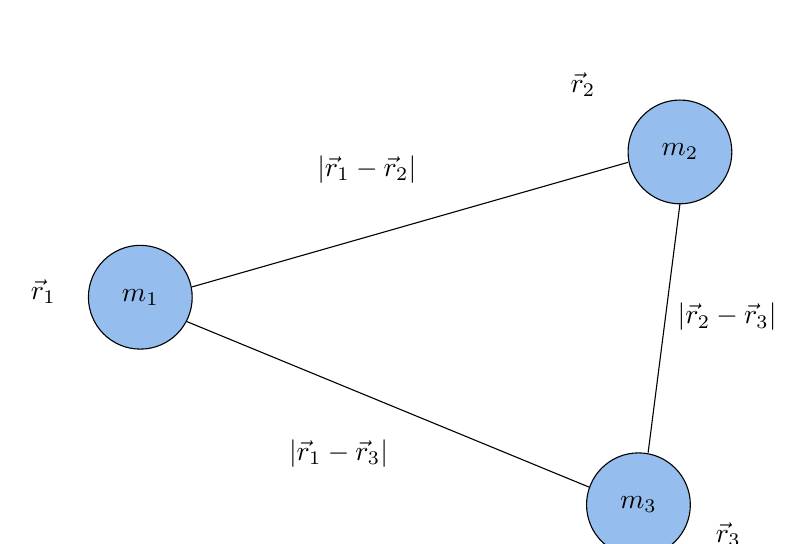
\begin{tikzpicture}[x=0.75pt,y=0.75pt,yscale=-1,xscale=1]
%uncomment if require: \path (0,300); %set diagram left start at 0, and has height of 300

%Shape: Circle [id:dp11919774335444377] 
\draw  [fill={rgb, 255:red, 74; green, 144; blue, 226 }  ,fill opacity=0.59 ] (120,135) .. controls (120,121.19) and (131.19,110) .. (145,110) .. controls (158.81,110) and (170,121.19) .. (170,135) .. controls (170,148.81) and (158.81,160) .. (145,160) .. controls (131.19,160) and (120,148.81) .. (120,135) -- cycle ;
%Shape: Circle [id:dp1512759538865308] 
\draw  [fill={rgb, 255:red, 74; green, 144; blue, 226 }  ,fill opacity=0.59 ] (360,235) .. controls (360,221.19) and (371.19,210) .. (385,210) .. controls (398.81,210) and (410,221.19) .. (410,235) .. controls (410,248.81) and (398.81,260) .. (385,260) .. controls (371.19,260) and (360,248.81) .. (360,235) -- cycle ;
%Shape: Circle [id:dp4443678325062712] 
\draw  [fill={rgb, 255:red, 74; green, 144; blue, 226 }  ,fill opacity=0.59 ] (380,65) .. controls (380,51.19) and (391.19,40) .. (405,40) .. controls (418.81,40) and (430,51.19) .. (430,65) .. controls (430,78.81) and (418.81,90) .. (405,90) .. controls (391.19,90) and (380,78.81) .. (380,65) -- cycle ;
%Straight Lines [id:da963502184755707] 
\draw    (170,130) -- (380,70) ;
%Straight Lines [id:da5114822387415651] 
\draw    (167.27,146.68) -- (361.67,226.68) ;
%Straight Lines [id:da3674207943033927] 
\draw    (405,90) -- (389.67,209.88) ;

% Text Node
\draw (145,135) node    {$m_{1}$};
% Text Node
\draw (385,235) node    {$m_{3}$};
% Text Node
\draw (405,65) node    {$m_{2}$};
% Text Node
\draw (91,125.4) node [anchor=north west][inner sep=0.75pt]    {$\vec{r}_{1}$};
% Text Node
\draw (421,242.4) node [anchor=north west][inner sep=0.75pt]    {$\vec{r}_{3}$};
% Text Node
\draw (351,25.4) node [anchor=north west][inner sep=0.75pt]    {$\vec{r}_{2}$};
% Text Node
\draw (229,65.4) node [anchor=north west][inner sep=0.75pt]    {$|\vec{r}_{1} -\vec{r}_{2} |$};
% Text Node
\draw (215.4,202.2) node [anchor=north west][inner sep=0.75pt]    {$|\vec{r}_{1} -\vec{r}_{3} |$};
% Text Node
\draw (402.6,136.6) node [anchor=north west][inner sep=0.75pt]    {$|\vec{r}_{2} -\vec{r}_{3} |$};

\end{tikzpicture}

    \caption{3 Particle Rigid Body}
    \label{fig:rigid body 3 particle}
\end{figure}

So, we have 3 constraint equations in a system with 9 particles. This gives a total of $3N-3=6$-\gls{dof}. When any additional particles are added, they must be fully constrained in all 3 translational degrees of freedom by constraints between $r_1$,$r_2$, and $r_3$. So, we always have constraints of the form $3N-3(N-2)$ for a rigid body. This is why we always see a rigid body displaying 6-\gls{dof}. We can then, of course, parametrize this in general coordinates with the cartesian coordinates and 3 angles.

\subsubsection{Minimal Set of Constraints}

\newglossaryentry{holonomic sys}
{
    name=holonomic system,
    first = {\textit{holonomic system}},
    description={A system that is entirely composed of holonomic constraints},
    see={holonomic const}
}
So far, we have only discussed holonomic constraints, those that are related to position or on the generalized parameters, and possibly have some relation in time. When a system is a \gls{holonomic sys}, that is, purely defined by \glspl{holonomic const}, it is always possible to find a set of $\mathcal{M}$ generalized parameters to describe the particle motion. In other words, the minimum number of parameters is equivalent to the number of degrees of freedom in the system.

That said, we often choose to use more parameters, particularly in the case of rotations. As we will see in Volume II, we often find it more useful to use a non-minimal set of constraints to encode rotations for reasons to avoid singularities in the solution.

It is also common to see a non-minimal set of constraints used when the minimal set is cumbersome and does not give an intuitive feel to the problem.
\subsubsection{Non-Holonomic Constraints}

\newglossaryentry{non holo const}
{
    name=non-holonomic constraint,
    first = {\textit{non-holonomic constraint}},
    description={A constraint that depends on more than the position of the particles in the system},
    see={holonomic const}
}
The other class of constraints are those constraints that are not merely a function of the generalized coordinates. These constraints, called \glspl{non holo const}, define the set of all constraints that depend on more than just the position of particles. This is a huge class of constraints so we will not cover every type. These are also less important to our derivations so we will only briefly discuss them.

\newglossaryentry{gen vel}
{
    name=generalized velocity,
    first = {\textit{generalized velocity}},
    plural = {generalized velocities},
    firstplural = {\textit{generalized velocities}},
    description={A free direction of movement for a vehicle. These can be translational or rotational directions}
}

The most common among these, and where we will focus our attention here, is constraints on the time derivative of the generalized coordinates. These are called \glspl{gen vel}, denoted $\dot{q}_j$. Such an example of a constraint on \glspl{gen vel} is a roller skate. A roller stake only allows a velocity in the direction of the skate and restricts velocity along the direction normal to the roller stake.

One important thing about non-holonomic constraints is that they do not reduce the number of parameters needed to define the system. 

%add more if needed.
\subsection{Lagrange's Equation in Generalized Coordinates}

The good thing about the \gls{Lagrangian} method is that it is invariant to changes in our coordinate system. Because the \gls{Lagrangian} is an equation of energy, and energy is independent of coordinate transformations, we can easily express the Euler-Lagrange equation in generalized coordinates with little hassle.

Using the generalized coordinates, the kinetic energy is a function of the generalized positions, velocities, and time. The potential is a function of the generalized position and time, so the \gls{Lagrangian} becomes:
$$L\equiv T-U=T(q_j,\dot{q}_j,t)-U(q_j,t)$$
Stated another way, the \gls{Lagrangian} is a function of the generalized positions, velocities, and time, as $L=L(q_j,\dot{q}_j,t)$. The Euler-Lagrange Equation then becomes:
\begin{gather}\label{eq:Euler-Lagrange General}
\color{blue}\boxed{\color{black}\frac{\partial L}{\partial q_j}-\frac{d}{dt}\frac{\partial L}{\partial \dot{q}_j}=0,\ \ \ j=1,2,\cdots M}\\
\mathrm{\color{blue}Generalized \ Euler-Lagrange \ Equations}
\end{gather}
Next we will show a problem where the rotational invariance and generalized coordinates proves especially useful in simplifying our derivation:
\subsection{Pendulum EOM Derivation}
\subsubsection{Problem Set-Up}
Suppose we have a pendulum of length L. The mass is rigidly attached to the pendulum. A reference frame $a$ that moves with the pendulum is shown in Figure \ref{fig:Pendulum}. The inertial frame is also shown. The pendulum moves in only the $xy$ plane.
\begin{figure}[ht]

\centering

\tikzset{every picture/.style={line width=0.75pt}} %set default line width to 0.75pt        

\begin{tikzpicture}[x=0.75pt,y=0.75pt,yscale=-1,xscale=1]
%uncomment if require: \path (0,300); %set diagram left start at 0, and has height of 300

%Straight Lines [id:da8354203825727349] 
\draw    (320,60) -- (420,240) ;
\draw [shift={(320,60)}, rotate = 60.95] [color={rgb, 255:red, 0; green, 0; blue, 0 }  ][fill={rgb, 255:red, 0; green, 0; blue, 0 }  ][line width=0.75]      (0, 0) circle [x radius= 2.68, y radius= 2.68]   ;
%Shape: Arc [id:dp31284247913451657] 
\draw  [draw opacity=0] (403.12,208.97) .. controls (378.54,222.36) and (350.19,230) .. (320,230) -- (320,65) -- cycle ; \draw [color={rgb, 255:red, 74; green, 144; blue, 226 }  ,draw opacity=1 ]   (400.15,210.55) .. controls (376.27,222.96) and (348.98,230) .. (320,230) ; \draw [shift={(320,230)}, rotate = 357.91] [color={rgb, 255:red, 74; green, 144; blue, 226 }  ,draw opacity=1 ][line width=0.75]    (0,5.03) -- (0,-5.03)   ; \draw [shift={(403.12,208.97)}, rotate = 153.52] [fill={rgb, 255:red, 74; green, 144; blue, 226 }  ,fill opacity=1 ][line width=0.08]  [draw opacity=0] (8.04,-3.86) -- (0,0) -- (8.04,3.86) -- cycle    ;
%Shape: Circle [id:dp5099783674397224] 
\draw  [color={rgb, 255:red, 0; green, 0; blue, 0 }  ,draw opacity=1 ][fill={rgb, 255:red, 74; green, 74; blue, 74 }  ,fill opacity=1 ] (410,240) .. controls (410,234.48) and (414.48,230) .. (420,230) .. controls (425.52,230) and (430,234.48) .. (430,240) .. controls (430,245.52) and (425.52,250) .. (420,250) .. controls (414.48,250) and (410,245.52) .. (410,240) -- cycle ;
%Straight Lines [id:da8713569921261672] 
\draw [color={rgb, 255:red, 208; green, 2; blue, 27 }  ,draw opacity=1 ]   (340,50) -- (438.54,227.38) ;
\draw [shift={(440,230)}, rotate = 240.95] [fill={rgb, 255:red, 208; green, 2; blue, 27 }  ,fill opacity=1 ][line width=0.08]  [draw opacity=0] (8.93,-4.29) -- (0,0) -- (8.93,4.29) -- cycle    ;
\draw [shift={(340,50)}, rotate = 240.95] [color={rgb, 255:red, 208; green, 2; blue, 27 }  ,draw opacity=1 ][line width=0.75]    (0,5.59) -- (0,-5.59)   ;
%Straight Lines [id:da9538559670922312] 
\draw    (200,240) -- (200,202) ;
\draw [shift={(200,200)}, rotate = 90] [color={rgb, 255:red, 0; green, 0; blue, 0 }  ][line width=0.75]    (7.65,-2.3) .. controls (4.86,-0.97) and (2.31,-0.21) .. (0,0) .. controls (2.31,0.21) and (4.86,0.98) .. (7.65,2.3)   ;
%Straight Lines [id:da3275390122881038] 
\draw    (200,240) -- (238,240) ;
\draw [shift={(240,240)}, rotate = 180] [color={rgb, 255:red, 0; green, 0; blue, 0 }  ][line width=0.75]    (7.65,-2.3) .. controls (4.86,-0.97) and (2.31,-0.21) .. (0,0) .. controls (2.31,0.21) and (4.86,0.98) .. (7.65,2.3)   ;
%Straight Lines [id:da24072013587186947] 
\draw [color={rgb, 255:red, 208; green, 2; blue, 27 }  ,draw opacity=1 ]   (451.54,222.12) -- (470.54,255.03) ;
\draw [shift={(471.54,256.77)}, rotate = 240] [color={rgb, 255:red, 208; green, 2; blue, 27 }  ,draw opacity=1 ][line width=0.75]    (7.65,-2.3) .. controls (4.86,-0.97) and (2.31,-0.21) .. (0,0) .. controls (2.31,0.21) and (4.86,0.98) .. (7.65,2.3)   ;
%Straight Lines [id:da7099456662568205] 
\draw [color={rgb, 255:red, 208; green, 2; blue, 27 }  ,draw opacity=1 ]   (451.54,222.12) -- (484.45,203.12) ;
\draw [shift={(486.18,202.12)}, rotate = 150] [color={rgb, 255:red, 208; green, 2; blue, 27 }  ,draw opacity=1 ][line width=0.75]    (7.65,-2.3) .. controls (4.86,-0.97) and (2.31,-0.21) .. (0,0) .. controls (2.31,0.21) and (4.86,0.98) .. (7.65,2.3)   ;


% Text Node
\draw (362,227.4) node [anchor=north west][inner sep=0.75pt]  [color={rgb, 255:red, 74; green, 144; blue, 226 }  ,opacity=1 ]  {$\theta $};
% Text Node
\draw (391,122.4) node [anchor=north west][inner sep=0.75pt]  [color={rgb, 255:red, 208; green, 2; blue, 27 }  ,opacity=1 ]  {$L$};
% Text Node
\draw (241,228.4) node [anchor=north west][inner sep=0.75pt]    {$\hat{x}$};
% Text Node
\draw (197,176.4) node [anchor=north west][inner sep=0.75pt]    {$\hat{y}$};
% Text Node
\draw (481.25,191.58) node [anchor=north west][inner sep=0.75pt]  [color={rgb, 255:red, 208; green, 2; blue, 27 }  ,opacity=1 ,rotate=-330]  {$\hat{a}_{\theta }$};
% Text Node
\draw (467.54,261.84) node [anchor=north west][inner sep=0.75pt]  [color={rgb, 255:red, 208; green, 2; blue, 27 }  ,opacity=1 ,rotate=-330]  {$\hat{a}_{r}$};

\end{tikzpicture}

    \caption{Pendulum Set-Up}
    \label{fig:Pendulum}
\end{figure}
\subsubsection{Newtonian Approach}
You have likely seen the Newtonian approach many times, but we show it here for completeness and to contrast the approach with the \gls{Lagrangian} more directly. 

In the Newtonian Approach to deriving EOM's, we always start with the forces governing the system. In this case, we have two forces. The gravitational force, $mg$, acts in the $-\hat{y}$-direction and the tension force acts in the $-\hat{a}_r$-direction. From the constraint on length, the acceleration in the $\hat{a}_r$ must be zero. Thus, the component of gravity in the $\hat{a}_r$ direction must equal the tension.

We express the gravity in the $a$-frame to find this:
$$\hat{y}=-\cos\theta\hat{a}_r+\sin\theta \hat{a}_\theta$$
So, by balancing the forces in the $\hat{a}_r$-direction:
$$m{\ddot{a}}_r=mg\cos\theta \hat{a}_r-\vec{F}_T$$
In the $\hat{a}_\theta$-direction, we have unconstrained motion, so $\sum\vec{F}=m\vec{a}$. Our force equation is thus: 
$$F=-mg\sin\theta\hat{a}_{\theta}$$
Next, we need to find our acceleration in the inertial frame using the \gls{bke} to solve the RHS of the force balance. Starting with the position vector:
$$\vec{r}^{\ op}=L\hat{a}_r$$
We can apply the \gls{bke} to find our inertial velocity:
$${}^i\vec{v}^p={}^a\frac{d}{dt}\vec{r}^{\ op}+{}^i\omega^a\times\vec{r}^{\ op}$$
Plugging in appropriate quantities:
$${}^i\vec{v}^p={}^a\frac{d}{dt}(L\hat{a}_r)+\dot{\theta}\hat{a}_3\times(L\hat{a}_r)$$
$${}^i\vec{v}^p=\dot{\theta}L\hat{a}_\theta$$
We do this again to find the inertial acceleration:
$${}^i\vec{a}^p={}^a\frac{d}{dt}{}^i\vec{v}^p+{}^i\omega^a\times{}^i\vec{v}^p$$
$${}^i\vec{a}^p={}^a\frac{d}{dt}{}\dot{\theta}L\hat{a}_\theta+\dot{\theta}\hat{a}_3\times\dot{\theta}L\hat{a}_\theta$$
$${}^i\vec{a}^p=\ddot{\theta}L\hat{a}_\theta-\dot{\theta}^2L\hat{a}_r$$
Now, we equate the forces in each direction:
$$-mg\sin\theta\hat{a}_\theta=\ddot{\theta}L\hat{a}_\theta$$
Rearranging, we arrive at our \gls{eom}:
$$\ddot{\theta}+\frac{g}{L}\sin\theta=0$$
\subsubsection{Lagrangian Approach}
In the \gls{Lagrangian} approach, we will start by defining our constraints and coordinates. Some preliminary analysis shows that using polar coordinates for this problem will be useful. If we do not recognize this, we can always convert later (a distinct advantage of the \gls{Lagrangian} approach, since it is coordinate frame invariant). Here we will choose a cylindrical coordinate systsem:
\begin{gather}
    q_1=r\\q_2=\theta\\q_3=z
\end{gather}
Next, we define constraints. Since there is no motion in the z-axis:
$$z=0$$
And the constraint on the length gives us:
$$q_1-L=0$$
So, we have 1 \gls{dof} from \eqref{eq:dof}. Since both $z$ and $r$ are constrained, we can express our \gls{eom} in terms of one generalized coordinate, $\theta$.

Next, we define the \gls{Lagrangian}. Knowing that the linear velocity of the particle is $\dot{\theta}L$, we get:
$$T=\frac{1}{2}m\dot{\theta}^2L^2$$
For the potential, we choose the origin as our reference, giving us:
$$U=-mgy$$
And a coordinate transformation into polar using $y=r\cos\theta$ yields:
$$U=-mgL\cos\theta$$
This gives the \gls{Lagrangian}:
$$L=\frac{1}{2}m\dot{\theta}^2L^2+mgL\cos\theta$$
Applying the Euler-Lagrange formula for generalized coordinates, \eqref{eq:Euler-Lagrange General} on the single generalized coordinate:
\begin{gather}
    \frac{\partial L}{\partial \theta}=-mgL\sin\theta\\
    \frac{\partial L}{\partial \dot{\theta}}=mL^2\dot{\theta}\\
    \frac{d}{dt}\left(mL^2\dot{\theta}\right)=mL^2\ddot{\theta}
\end{gather}
So, the final system is:
$$-mgL\cos\theta -mL^2\ddot{\theta}=0$$
With some rearrangement:
$$\ddot{\theta}+\frac{g}{L}\sin\theta=0$$
We notice that with the \gls{Lagrangian} approach, we did not need to have an understanding of the vector directions, frame translations, or \gls{bke} to find our \gls{eom}. This, in addition to the flexibility of the generalized coordinates, is the real power of this approach.

\section{Generalized Forces}

\section{Hamiltonian Mechanics}
After the formulation of \gls{Lagrangian} Mechanics, another formulation was created by Hamilton later on. The Hamiltonian formulation, like the \gls{Lagrangian}, does not introduce any new concepts, because it is simply an alternate approach to dynamics. However, like the \gls{Lagrangian}, it makes some types of problems more simple. We present the Hamiltonian here briefly for its use case in \glspl{symplectic int}.
\subsection{Derivation of the Hamiltonian}
The exact derivation of the Hamiltonian using Legendre transforms is beyond the scope of our present discussion, so we will mostly discuss the consequences of this derivation. 

\newglossaryentry{gen momenta}
{
    name=generalized momenta,
    first = {\textit{action}},
    description={The time integral of energy is known as the action, which is often denoted $S$}
}

The Hamiltonian method replaces the generalized velocities with \textit{generalized momenta}. The generalized momenta are a function of $q,\dot{q},$ and $t$. We express the generalized momenta as $p$. $p$ is defined to be:
$$p(q,\dot{q},t)\equiv\dfrac{\partial L}{\partial \dot{q}_i}$$
Thus, we express our Hamiltonian, $\mathcal{H}$, in terms of the generalized positions, generalized momenta, and time. This looks like:
$$\mathcal{H}=\mathcal{H}(q_j,p_j,t)$$
In a conservative system, we can also write: $$\mathcal{H}=T+U$$
Using relations with the \gls{Lagrangian}, we can write two first order differential equations for the \gls{eom} with the Hamiltonian.

\begin{gather}
\color{blue}\boxed{
\begin{array}{r}\color{black}
     \dot{q}_k=\dfrac{\partial \mathcal{H}}{\partial p_k}\\
     \color{black}
  -\dot{p}_k=\dfrac{\partial \mathcal{H}}{\partial q_k}
\end{array}
}\\
\color{blue}\mathrm{Hamiltonian \ EOM's}
\end{gather}
This is all we will note about Hamiltonian Mechanics for now. We will note here that these are more useful in the case of numerical integration because these are first order differential equations, as opposed to the second order differential equations of Lagrangian Mechanics.
\section{Lagrangian Derivation of Rigid Body Dynamics}

In Section \ref{Euler Rotation Equations}, we explored the Newtonian method of deriving the Euler rotation equations using the \gls{bke}. Here, we present an alternative derivation that utilizes the \gls{Lagrangian} approach and is ultimately a more fundemental and simple derivation.

We showed earlier in Section \ref{sec: rigid body constraints} that we can describe a rigid body system with 6 generalized parameters, three of which are angles.
\subsection{Torque Free Equations}
In the case of no applied torque, the derivations of Euler's Equations become surprisingly simple. We can assume that the change in height of the rigid body is irrelevant for pure rotation, so the \gls{Lagrangian} is simply the kinetic energy of the object. We can suppose that we are also in a coordinate system where the translational kinetic energy is 0. This gives:
\begin{equation}\label{eq:rigid body KE}
L=\frac{1}{2}I\omega^2
\end{equation}
We can select our generalized coordinates as the three Euler angles, $\psi$, $\theta$, and $\phi$ (see Section \ref{sec:Euler Angles}).

Selecting the generalized coordinate, $\psi$, as an example, the Euler-Lagrange equation gives:
$$\frac{\partial L}{\partial \psi}-\frac{d}{dt}\frac{\partial L}{\partial \dot{\psi}}=0$$
Using the derivation of the components of angular velocity using Euler Angles, we have:
\begin{gather}
\omega_1=\dot{\phi}\sin\theta\sin\psi+\dot{\theta}\cos\psi\\
    \omega_2=\dot{\phi}\sin\theta\cos\psi-\dot{\theta}\sin\psi\\
    \omega_3=\dot{\phi}\cos\theta+\dot{\psi}
\end{gather}
So, we can also express our \gls{Lagrangian} in terms of the angular acceleration:
$$\frac{\partial L}{\partial \omega_i}\frac{\partial \omega_i}{\partial \psi}-\frac{d}{dt}\frac{\partial L}{\partial \omega_i}\frac{\partial \omega_i}{\partial \dot{\psi}}=0$$
At this point, the derivation is simply a matter of 'plug and chug'. Calculating the derivatives with respect to $\psi$:
\begin{gather}
    \frac{\partial \omega_1}{\partial \psi}=-\dot{\phi}\sin\theta\cos\psi-\dot{\theta}\sin\psi\\
    \frac{\partial \omega_2}{\partial \psi}=-\dot{\phi}\sin\theta\sin\psi-\dot{\theta}\cos\psi\\
    \frac{\partial \omega_3}{\partial \psi}=0
\end{gather}
We notice here that $\frac{\partial \omega_1}{\partial \psi}=\omega_2$ and $\frac{\partial \omega_2}{\partial \psi}=-\omega_1$. Next, taking our derivatives with respect to $\dot{\psi}$:
\begin{gather}
    \frac{\partial \omega_1}{\partial \dot{\psi}}=0\\
    \frac{\partial \omega_2}{\partial \dot{\psi}}=0\\
    \frac{\partial \omega_3}{\partial \dot{\psi}}=1
\end{gather}
Last, we can make a substitution for the $\frac{\partial L}{\partial \omega_i}$ term by taking a derivative of the kinetic energy\eqref{eq:rigid body KE}:
$$\frac{\partial L}{\partial \omega_i}=I_i\omega_i$$
Plugging everything into the Euler-Lagrange formula, we have:
$$I_1\omega_1\omega_2-I_2\omega_1\omega_2-\frac{d}{dt}I_3\omega_3=0$$
Some simplification yields:
$$\left(I_1-I_2\right)\omega_1\omega_2=I_3\dot{\omega_3}$$
We can perform the analogous analysis for the other axes, yielding the full set of torque free rigid body equations:
\begin{gather}
\color{blue}\boxed{
\begin{array}{ll}
\color{black}
\left(I_2-I_3\right)\omega_2\omega_3=I_1\dot{\omega_1}
     &\\
     \color{black}\left(I_3-I_1\right)\omega_1\omega_3=I_2\dot{\omega_2}
     &\\
     \color{black}\left(I_1-I_2\right)\omega_1\omega_2=I_3\dot{\omega_3}
\end{array}}\\
\color{blue}
\mathrm{Torque-Free \ Rotations}
\end{gather}
\subsection{Forced Euler Rigid Body Dynamics}
\section{Key Ideas}
\begin{enumerate}
    \item We can find the \gls{eom} of a system using either the Newtonian approach or the \gls{Lagrangian} approach, and it is often easier to find an \gls{eom} using the \gls{Lagrangian} for a conservative system.
    \item The \gls{Lagrangian} is scalar, so it is invariant to coordinate transforms. This means we can choose any variables we want for our generalized coordinates when performing derivations.
    \item The methodology of Newtonian mechanics and \gls{Lagrangian} mechanics are fundementally different. Newtonian mechanics deals with the influence of external actions (forces), while \gls{Lagrangian} Mechanics emphasizes the internal state of the system.
    \item %add Hamiltonian v. Lagrangian
\end{enumerate}
\section{Further Reading}
The following section borrows heavily from the derivations of Chapter 6 and 7 of  \cite{thornton_classical_nodate} and Chapter 5 of  \cite{noauthor_variational_2017}. A good video overview of this topic can be found at \cite{veritasium_closest_2024}.

There are an abundance of sources for classical mechanics. We can personally recommend the video series at \cite{ross_lagranges_nodate}, which covers this material in a manner more suitable to engineering contexts.

\section{Practice Problems}
\begin{enumerate}
    \item Arthur keeps finding bugs on the apples that he is feeding his horse. Arthur heard that you have been learning about generalized coordinates. He wants a way to describe the position of the bugs on his apples using a minimal set of coordinates.

Find a suitable set of generalized coordinates to describe this system. Write out any equations of constraints of the system. \textit{Hint: A apple is topologically similar to a sphere!}

    \item You are a prominent mathematician in the year 1696. Bernoulli proposes a problem to you to find a curve from a point $(x_0,y_0)$ to another point $\left(x_f,y_f\right)$. When a particle is placed on this path, it should be a faster path than any other path the particle could take down the slope under the influence of only gravity.
%    \item brachistochrone
\begin{enumerate}
    \item Find the velocity as a function of the distance from the initial height, $h$, for the particle using energy conservation.
    \item Write a general expression for the amount of time it takes a particle to descent a path using an integral. \textit{Hint: you can write $t=\frac{ds}{v}$}.
    \item Use the Euler-Lagrange equation to solve for the form of this curve (You may find the integral form useful!). Plot the result.
\end{enumerate}

\item You have a pendulum attached to a cart that can move back and forth along the $\hat{x}$-axis. Derive the \gls{eom} of the system using energy methods.
\item You have a double pendulum with two rigid arms, both of length $l$, which are free to rotate in the $xy$-plane. Find the \gls{eom} for the system.

\end{enumerate}
\chapter{Computational Attitude Dynamics}\label{sec:attitude dynamics}
\begin{chapquote}{Lord Kelvin, 1892}
''Quaternions came from Hamilton after his really good work had been done; and, though beautifully ingenious, have been an unmixed evil to those who have touched them in any way, including Clerk Maxwell.''
\end{chapquote}

Attitude Dynamics is the math describing the orientation of a vehicle in space as the result of applied moments. Relying heavily on advanced mathematics, this concept is naturally more difficult to grasp. In fact, we have dedicated the entirety of Volume II to the theory behind attitude determination and dynamics. Derivations for everything from simple, two-dimensional problems and single-axis rotations to quaternions are included in that book. Following the core purpose of this volume, we will only be describing implementation of attitude dynamics using MATLAB functions. However, we highly recommend you break here to read the entirety of Volume II in order to gain a more definitive understanding what and more importantly why everything is happening with the code in this section.


\section{Euler Angles}\label{sec:Euler Angles}
\newglossaryentry{Euler angles}
{
    name=Euler angles,
    first = {\textit{Euler angles}},
    description={A group of three scalar values used to describe the orientation of a body in space}
}

The first method to express the orientation of a vehicle is through the use of Euler angles. These form the basis for our understanding of attitude, being the more intuitive method. As stated previously, the theory and derivations for everything you will use here is included in Volume II, which by now, we hope you've already seen! If you haven't, shame on you, but don't worry, we'll provide some basic definitions here to give you the bare bones of what is needed in the function calls.

First and most important, we use the 3-2-1 rotation sequence to determine Euler angles. This means we have an angle $\phi$ to describe the rotation about the $x$-axis, an angle $\theta$ to describe the rotation about the $y$-axis, and an angle $\psi$ to describe the rotation about the $z$-axis. The order we do these rotations in is Z-Y-X, or $\psi$-$\theta$-$\phi$. 

\subsection{The Direction Cosine Matrix}\label{sec:TheDCM}

To start, we want a way to easily convert any arbitrary vector from being described with one reference frame to another. We do this through the use of the Direction Cosine Matrix, or DCM. This allows us to take this matrix and multiply it with our vector in the inertial frame and obtain an identical vector in the body frame.

In MATLAB, there exists a function - "angle2dcm" - that creates this for us! By inputting the scalar values of our Euler angles (in radians!) as well as the chosen rotation sequence, MATLAB creates the DCM as an output, allowing us to multiply this matrix with our inertial vector we want to express in the body frame. Note the function allows an input of any number of rotations to find DCM's for. This is a fun little aspect of the function; however, it is irrelevant for our use as we input the new Euler angles every time-step during our "ode45" integration scheme. One additional thing to consider: the "angle2dcm" function returns the DCM as a transform from the inertial to the body frame. If we were to transform a vector from the body to inertial frame, we would need to take the transpose of the given matrix.

\subsection{Relating Euler Rates with Angular Velocity}

\newglossaryentry{Euler rates}
{
    name=Euler rates,
    first={\textit{Euler rates}},
    description={A way to describe rotational rates with orientation for 3-dimensional rotations, they are denoted by the dot of the corresponding Euler angle: ($\dot{\psi},\dot{\theta},\dot{\phi}$)}
}

One thing you might recall from reading Volume II is that integrating the angular velocities in a 3-dimensional case DOES NOT return the Euler angles. This job is left to Euler rates, something else we would like to include in our code. All you brilliant readers will also recall the existence of what we affectionately call the ''B'' matrix that allows us to use Euler angles to express a relation between Euler rates and angular velocities. Unfortunately, there doesn't exist a MATLAB function that can calculate the ''B'' matrix, leaving us to our own devices to construct one from scratch. Luckily, we already did the heavy lifting, meaning we can copy the matrix derived in Volume II straight into our MATLAB script. That matrix is as follows, for quick reference:
\begin{gather}
    \color{blue}\boxed{\color{black}B=\begin{bmatrix}
    1&tan(\theta)sin(\phi)&tan(\theta)cos(\phi)\\
    0&cos(\phi)&-sin(\phi)\\
    0&\dfrac{sin(\phi)}{cos(\theta)}&\dfrac{cos(\phi)}{cos(\theta)}
\end{bmatrix}}\\\color{blue}\mathrm{The\ ''B''\ Matrix\ for\ 3-2-1\ Rotations}
\end{gather}

\subsection{Euler Angle MATLAB Function Example}\label{sec:EulerDynamicsMATLABExample}

Putting it all together, we're going to write a simple code using Euler angles to practice using MATLAB's built in functions. Say we have a very important vector we want to express in the body frame and another important vector we want to express in the inertial frame: gravity and thrust respectively. If our rocket weighs 100 Newtons and outupts a thrust of 1000 Newtons, we know this appears in vector notation as: $-100\hat{x}$ and $-1000\hat{X}$. Consider a moment in time, when - using the 3-2-1 rotation sequence - our vehicle is at a roll angle of 2.71 radians and a yaw and pitch angles of 0.2 radians, where we want to convert our gravity vector from the inertial frame to the body frame. In addition, with knowledge that the angular velocity at that instant is $\begin{bmatrix}
    2.5&0.1&0.1
\end{bmatrix}^T$, we can also find the Euler rate of the system. The following code listing quickly runs through the process, with sufficient commentary within the script explaining every action taken.

\lstset{style=mystyle}

\lstinputlisting[language=Matlab, caption=Euler Angle Dynamics Example]{6DoF Explanation Scripts/Attitude Dynamics Examples/GravityToBodyEuler.m}\label{Euler Dynamics Listing}

Our results come out to be the following, with the gravity force expressed in the body frame and thrust expressed in the inertial frame as:
\begin{equation}
    ^b\vec{F}_{g}=\begin{bmatrix}
        -96.0530\\-26.1902\\9.3748
    \end{bmatrix};\ ^i\vec{F}_{T}=\begin{bmatrix}
        -960.5305\\-194.7092\\198.6693
    \end{bmatrix}
\end{equation}

At this point, we would use our numerical integration scheme to approximate the next timestep's Euler angles using the Euler rates we just found. We won't do that here, but you can see the implementation in the 6DoF itself or the Dzhanibekov example!


\section{Quaternions}\label{sec:quaternions}
\newglossaryentry{quaternion}
{
    name=quaternion,
    first = {\textit{quaternion}},
    description={An extension of the complex numbers with elements $j$ and $k$ added. The common form is expressed $q_1+q_2i+q_3j+q_4k$ (our notation) or $q_1i+q_2j+q_3k+q_4$. The algebra of quaternions is generally denoted $\mathbb{H}$}
}

\newglossaryentry{versor}
{
    name=versor,
    first = {\textit{versor}},
    description={The normalization of a quaternion and the only way to encode rotations, it is equivalent to $\frac{\vec{q}}{||\vec{q}||}$. Fun note on the etymology of the word: it is derived from the Latin word ''versari'' which means ''to turn'' among other translations. With the suffix ''-or'', it becomes a noun, taking the meaning ''the turner''}
}

\newglossaryentry{skew-symmetric matrix}
{
    name=skew-symmetric matrix,
    first = {\textit{skew-symmetric matrix}},
    description={A matrix which obeys the property that every $a_{ij}=-a_{ji}$. This can be interpreted to mean every term across the diagonal is equal in magnitude, but opposite in sign. Sometimes called an anti-symmetric matrix or anti-metric matrix}
}

To match industry/academia standards, our 6DoF model uses \glspl{quaternion}. The use of hyper-imaginary numbers allows us to avoid losing a degree of freedom at a specific orientation in our rocket (called \textit{gimbal lock}), making the simulation more robust. Just as with Euler angles, MATLAB has an extensive suite of functions that make the implementation of \glspl{quaternion} just as easy. 

\subsection{Quaternion Rotation Matrix}

We're going to combine a few initial steps of the code surrounding \gls{quaternion} attitude dynamics. To start, we want to convert from Euler angles to \glspl{quaternion}s, as Euler angles are more intuitive to define and initialize the simulation. MATLAB's function "eul2quat" does just that. By inputting the Euler angles in the appropriate sequence, along with the chosen rotation sequence (match the Euler angles with the order), the function returns the corresponding quaternion vector. 

Having initialized our quaternion vector, we can now use another MATLAB script to construct our DCM. The function "quat2dcm" takes the quaternion as an input, and returns the DCM at that instant. Incredibly simple and incredibly useful; however, we must once again consider that this DCM converts only from the inertial frame to the body frame. Meaning just as we had done with Euler angles, it is necessary to take the transpose (inverse) of the matrix if we want to transform from the body to the inertial frame.


\subsection{Quaternion Rates}\label{sec: quaternion rates}

Just as we had done for Euler angles with Euler rates, we want to find a vector of quaternion rates that allows us to integrate and obtain a new quaternion vector. Also just as with Euler angles, there is no MATLAB function allowing us to relate quaternion rates with angular velocity. But just as with Euler angles, we've already found the necessary matrix to do so! This equation is shown in \eqref{eq: quat rates}. So plugging it into our script is an easy fix to make this operation possible.

\begin{gather}\label{eq: quat rates}
    \color{blue}\boxed{\color{black}\dot{\textbf{q}}=\frac{1}{2}\begin{bmatrix}
        0&-\omega_x&-\omega_y&-\omega_z\\
        \omega_x&0&\omega_z&-\omega_y\\
        \omega_y&-\omega_z&0&\omega_x\\
        \omega_z&\omega_y&-\omega_x&0
    \end{bmatrix}\vec{q}}
    \\\mathrm{\color{blue}Quaternion \ Rates}
\end{gather}

\subsection{Quaternion MATLAB Function Example}

Let's take the exact same example as before. We have the force of gravity acting down equal to $-100\hat{x}$. We have a roll angle of 2.71 radians, yaw and pitch angles of 0.2 radians. We finally have an instantaneous angular velocity of $\begin{bmatrix}
    2.5&0.1&0.1
\end{bmatrix}^T$. Wanting to obtain the gravity vector expressed in the body frame instead of the inertial frame, this time we're going to use quaternions to do so. In addition, we're now going to find the quaternion rate at the given moment. The listing below does this, and is sufficiently explained in the comments between operations. Note: you should see numerous similarities, with some sections of the code identical to the previous. 

\lstset{style=mystyle}

\lstinputlisting[language=Matlab, caption=Quaternion Dynamics Example]{6DoF Explanation Scripts/Attitude Dynamics Examples/GravityToBodyQuat.m}\label{Quat Dynamics Listing}

Taking a look at the outputs this generates, we see our results come out to be the following, with the gravity force expressed in the body frame and thrust expressed in the inertial frame as:
\begin{equation}
    ^b\vec{F}_{g}=\begin{bmatrix}
        -96.0530\\-26.1902\\9.3748
    \end{bmatrix};\ ^i\vec{F}_{T}=\begin{bmatrix}
        -960.5305\\-194.7092\\198.6693
    \end{bmatrix}
\end{equation}
A quick note about this script in relation to the other: the results shown above and the results shown in Section \ref{sec:EulerDynamicsMATLABExample} are identical. This gives confidence that we've implemented MATLAB's functions correctly. And once agian, at this point, we would use our numerical integration scheme to approximate the next timestep's quaternion using the quaternion rates we just found. We won't do that here, but as a reminder, you can see the implementation in the 6DoF itself or the Dzhanibekov example! 

\section{3D Rotation Example: Dzhanibekov effect}\label{sec:Dzhan}

\newglossaryentry{dzhan}
{
    name={Dzhanibekov Effect},
    first=\textit{Dzhanibekov Effect},
    description={A phenomenon in which rotation about an intermediate axis results in rotation about another axis. This phenomenon occurs with any body where the three PMOIs are not equal. It is easily seen with a tennis racket or a cell phone},
    see={pmoi}
}
To help digest the complex nature of attitude dynamics, a full example is especially useful. One of the consequences of Euler's Equations described %eqref equation above
above is that rotation about an intermediate axis is unstable. This effect is known as the Intermediate Axis Theorem or the \gls{dzhan}.

This is a good phenomenon to describe 3D rotations because it requires us to put together lots of knowledge throughout this section. Because our object rotates about all three axes, we must parametrize our rotation with \glspl{quaternion} to avoid possible singularities in the solution.

Before we can describe our system dynamics, we need to establish our coordinate system for this problem.

\begin{figure}[ht]
    \centering


\tikzset{every picture/.style={line width=0.75pt}} %set default line width to 0.75pt        

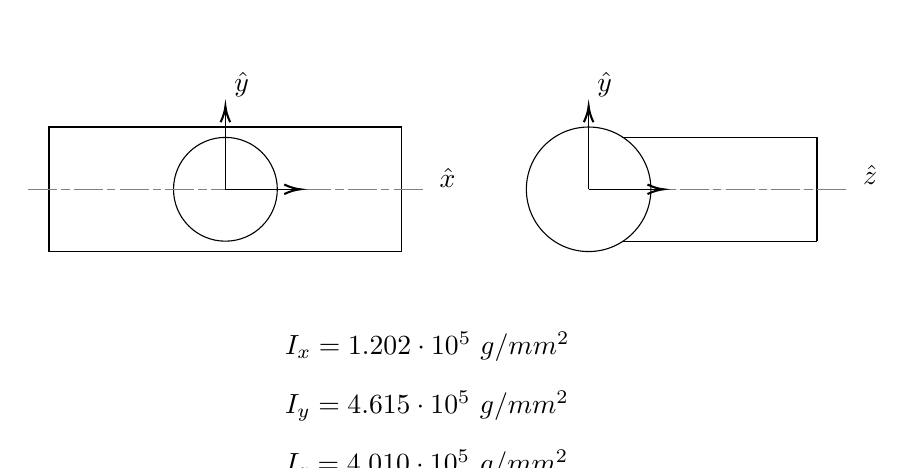
\begin{tikzpicture}[x=0.75pt,y=0.75pt,yscale=-1,xscale=1]
%uncomment if require: \path (0,300); %set diagram left start at 0, and has height of 300


%Shape: Circle [id:dp7493270463079389] 
\draw   (195,100) .. controls (195,86.19) and (206.19,75) .. (220,75) .. controls (233.81,75) and (245,86.19) .. (245,100) .. controls (245,113.81) and (233.81,125) .. (220,125) .. controls (206.19,125) and (195,113.81) .. (195,100) -- cycle ;
%Shape: Rectangle [id:dp8745965352536226] 
\draw   (135,70) -- (305,70) -- (305,130) -- (135,130) -- cycle ;
%Straight Lines [id:da5356768971699141] 
\draw [color={rgb, 255:red, 128; green, 128; blue, 128 }  ,draw opacity=1 ] [dash pattern={on 10.5pt off 1.5pt on 3pt off 1.5pt}]  (125,100) -- (315,100) ;
%Shape: Circle [id:dp11124327189723426] 
\draw   (365,100) .. controls (365,83.43) and (378.43,70) .. (395,70) .. controls (411.57,70) and (425,83.43) .. (425,100) .. controls (425,116.57) and (411.57,130) .. (395,130) .. controls (378.43,130) and (365,116.57) .. (365,100) -- cycle ;
%Straight Lines [id:da07234932776274916] 
\draw    (220,100) -- (220,62) ;
\draw [shift={(220,60)}, rotate = 90] [color={rgb, 255:red, 0; green, 0; blue, 0 }  ][line width=0.75]    (7.65,-2.3) .. controls (4.86,-0.97) and (2.31,-0.21) .. (0,0) .. controls (2.31,0.21) and (4.86,0.98) .. (7.65,2.3)   ;
%Straight Lines [id:da6659026149277345] 
\draw    (220,100) -- (254,100) ;
\draw [shift={(256,100)}, rotate = 180] [color={rgb, 255:red, 0; green, 0; blue, 0 }  ][line width=0.75]    (7.65,-2.3) .. controls (4.86,-0.97) and (2.31,-0.21) .. (0,0) .. controls (2.31,0.21) and (4.86,0.98) .. (7.65,2.3)   ;
%Straight Lines [id:da8158592711011072] 
\draw    (411,75) -- (505,75) ;
%Straight Lines [id:da1507348050424776] 
\draw    (411,125) -- (505,125) ;
%Straight Lines [id:da9455565481798273] 
\draw    (505,125) -- (505,75) ;
%Straight Lines [id:da5972499541109577] 
\draw [color={rgb, 255:red, 128; green, 128; blue, 128 }  ,draw opacity=1 ][fill={rgb, 255:red, 128; green, 128; blue, 128 }  ,fill opacity=1 ] [dash pattern={on 10.5pt off 1.5pt on 3pt off 1.5pt}]  (395,100) -- (520,100) ;
%Straight Lines [id:da4230804170313147] 
\draw    (395,100) -- (395,62) ;
\draw [shift={(395,60)}, rotate = 90] [color={rgb, 255:red, 0; green, 0; blue, 0 }  ][line width=0.75]    (7.65,-2.3) .. controls (4.86,-0.97) and (2.31,-0.21) .. (0,0) .. controls (2.31,0.21) and (4.86,0.98) .. (7.65,2.3)   ;
%Straight Lines [id:da58307827964758] 
\draw    (395,100) -- (429,100) ;
\draw [shift={(431,100)}, rotate = 180] [color={rgb, 255:red, 0; green, 0; blue, 0 }  ][line width=0.75]    (7.65,-2.3) .. controls (4.86,-0.97) and (2.31,-0.21) .. (0,0) .. controls (2.31,0.21) and (4.86,0.98) .. (7.65,2.3)   ;


% Text Node
\draw (322,88.4) node [anchor=north west][inner sep=0.75pt]    {$\hat{x}$};
% Text Node
\draw (223,42.4) node [anchor=north west][inner sep=0.75pt]    {$\hat{y}$};
% Text Node
\draw (398,42.4) node [anchor=north west][inner sep=0.75pt]    {$\hat{y}$};
% Text Node
\draw (526,87.4) node [anchor=north west][inner sep=0.75pt]    {$\hat{z}$};
% Text Node
\draw (247.5,167.4) node [anchor=north west][inner sep=0.75pt]    {$I_{x} =1.202\cdot 10^{5} \ g/mm^{2}$};
% Text Node
\draw (247.5,195.9) node [anchor=north west][inner sep=0.75pt]    {$I_{y} =4.615\cdot 10^{5} \ g/mm^{2}$};
% Text Node
\draw (247.5,224.4) node [anchor=north west][inner sep=0.75pt]    {$I_{z} =4.010\cdot 10^{5} \ g/mm^{2}$};


\end{tikzpicture}

    \caption{Non-Symmetric Body for Demonstrating Dzhanibekov Effect}
    \label{fig:Dzhan}
\end{figure}

\subsection{State Vector}
We'll start by describing our \gls{state vector} and initial conditions for this problem:

We define our original position is at the origin, giving us a position vector:
$$\vec{r}_0=\begin{bmatrix}
    0\\0\\0
\end{bmatrix}$$
We also define the initial velocity to be zero, giving a velocity vector:
$$\vec{v}_0=\begin{bmatrix}
    0\\0\\0
\end{bmatrix}$$
We also need an initial orientation. We can either directly initialize a \gls{quaternion} or write our initial orientation with \gls{Euler angles} and then convert to \glspl{quaternion}. Often, \gls{Euler angles} are more intuitive, so we will use these for our initialization. We can define an initial angle of all zeros, meaning that our body frame axes are initially coincident with the inertial frame. This gives \gls{Euler angles} of:
$$\begin{bmatrix}
    \phi\\\theta\\\psi
\end{bmatrix} =
\begin{bmatrix}
    0\\0\\0
\end{bmatrix}$$
Using the command "eul2quat" with a specification of "XYZ" for the frame, the initial \gls{quaternion} vector is given as:
$$\vec{q}_0=\begin{bmatrix}
    1\\0\\0\\0
\end{bmatrix}$$
Lastly, we need to describe the initial angular velocity. To properly demonstrate the effect, we need a small perturbation on our non-intermediate axes. We can write our omega vector as:
$$\vec{\omega}_0=\begin{bmatrix}
0.05\\0.05\\\pi
\end{bmatrix} rad/s$$

Putting all of the together, we arrive at our \gls{state vector}:
$$\vec{X}_0=\begin{bmatrix}
    \vec{r}_0\\\vec{v}_0\\\vec{\omega}_0\\\vec{q}_0
\end{bmatrix}$$
Which we can expand to the full form as a 13-element column vector:
$$\vec{X}_0=\begin{bmatrix}
    0\\0\\0\\0\\0\\0\\0.05\\0.05\\\pi\\1\\0\\0\\0
\end{bmatrix}$$
\subsection{Forces and Moments}
We can assume that we are operating in a 0-g environment (as this is where the effect is most prevalent) and that no body forces are acting on the object. We will also assume that air resistance in negligible and there are no losses. These assumptions mean that there are no forces that the acting on our body. Additionally, there are no moments on the body either. We have chosen this case for our example so that we can focus solely on the attitude dynamics.
\subsection{Attitude Dynamics}
Our attitude dynamics are fairly simple since there are no moments acting on the body. Our equations for the angular velocity rates in \eqref{eq: moment eq 2} reduce to the torque free equations:
\begin{gather}\label{eq: moment eq dzhan}
    \dot{\omega}_x=\frac{\left(I_y-I_z\right)\omega_y\omega_z}{I_x}\\
    \dot{\omega}_y=\frac{\left(I_z-I_x\right)\omega_z\omega_x}{I_y}\\
    \dot{\omega}_z=\frac{\left(I_x-I_y\right)\omega_y\omega_x}{I_z}
\end{gather}
To find our \gls{quaternion} rates, we simply use the same methods as in Section \ref{sec: quaternion rates}. This gives us:
\begin{gather}
{\color{black}\dot{\textbf{q}}=\frac{1}{2}\begin{bmatrix}
        0&-\omega_x&-\omega_y&-\omega_z\\
        \omega_x&0&\omega_z&-\omega_y\\
        \omega_y&-\omega_z&0&\omega_x\\
        \omega_z&\omega_y&-\omega_x&0
    \end{bmatrix}\vec{q}}
\end{gather}
\subsection{Translating to Code}
With all of these defined, we can write the derivative of our \gls{state vector} as:
\begin{equation}
    \dot{\textbf{X}}=\begin{bmatrix}
        \vec{v}\\\vec{a}\\\vec{\alpha}\\\dot{\textbf{q}}
    \end{bmatrix}
\end{equation}
From here, we can implement this in "ode45". We show all of the code for this model in the appendix.

Our initialization of the \gls{state vector} and all of the basic setup in contained in the main file, shown in listing \ref{code:DzhanMain}. The code that gets the derivative of the \gls{state vector} is the function passed into ode45. This code is shown in listing \ref{code:DzhanInt}. There is additionally a file to display the rotation of the body in an animation, which is shown in listing \ref{code:DzhanRotVis}.

%% add listings.
\section{Key Ideas}
\begin{enumerate}
    \item Read Volume II to learn more.
    \item Rotations can be encoded in a variety of ways, but the most useful and compact encoding of rotations involves the use of complex numbers.
    \item The use of MATLAB's built in suite of functions is incredibly useful in the implementation of attitude dynamics in 6DoF modeling.
    \item Be sure to keep your chosen rotation sequence straight when utilizing MATLAB's functions, and be sure to have a thorough understanding of how these functions work!
    \item No matter which style of describing rotations we choose - Euler angles or quaternions - they both result in identical answers
\end{enumerate}
\section{Further Reading}

Wertz

That one website

Some other horseshit

\section{Practice Problems}


\begin{enumerate}
    \item Your friend Jimothy, impressed by your MATLAB skills, has challenged you to model a spinning top. The top is axially symmetric about its $\hat{X}$-axis and has an initial spin rate of 1200 rpm and has an initial angle to the vertical of $20\degree$. The top spins down at a rate governed by an exponential decay of form $\omega(t)=\omega_0e^{\frac{1}{10}\ln(2)t}$ such that the spin rate is halved every 10 seconds. Gravity acts on the top in the negative $\hat{x}$-direction. The top has a mass of 20 grams. Relevant details are given in Figure \ref{fig:Spinning Top}.
Define any additional quantities that you deem necessary to solve the problem.

\begin{figure}[ht]
    \centering
    



\tikzset{every picture/.style={line width=0.75pt}} %set default line width to 0.75pt        

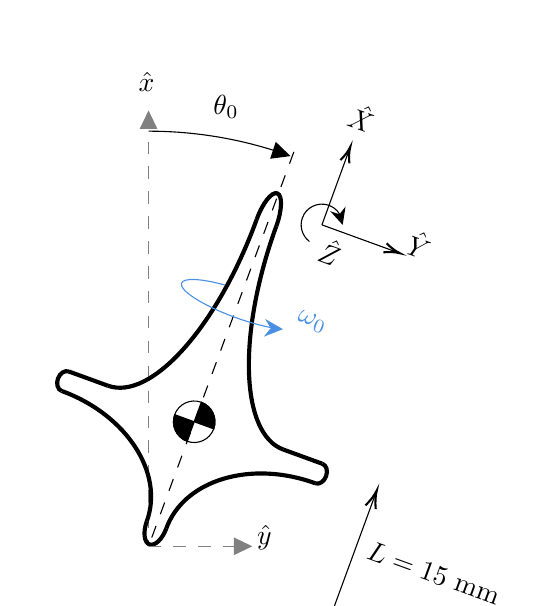
\begin{tikzpicture}[x=0.75pt,y=0.75pt,yscale=-1,xscale=1]
%uncomment if require: \path (0,300); %set diagram left start at 0, and has height of 300

%Straight Lines [id:da0769742316105797] 
\draw [color={rgb, 255:red, 128; green, 128; blue, 128 }  ,draw opacity=1 ] [dash pattern={on 4.5pt off 4.5pt}]  (330,33) -- (330,240) ;
\draw [shift={(330,30)}, rotate = 90] [fill={rgb, 255:red, 128; green, 128; blue, 128 }  ,fill opacity=1 ][line width=0.08]  [draw opacity=0] (8.93,-4.29) -- (0,0) -- (8.93,4.29) -- cycle    ;
%Straight Lines [id:da1132170918389106] 
\draw  [dash pattern={on 4.5pt off 4.5pt}]  (400,50) -- (330,240) ;
%Shape: Arc [id:dp36125796323627934] 
\draw  [draw opacity=0] (330,40) .. controls (354.03,40) and (377.08,44.24) .. (398.42,52.01) -- (330,240) -- cycle ; \draw    (330,40) .. controls (353.07,40) and (375.23,43.91) .. (395.85,51.09) ; \draw [shift={(398.42,52.01)}, rotate = 198.33] [fill={rgb, 255:red, 0; green, 0; blue, 0 }  ][line width=0.08]  [draw opacity=0] (8.93,-4.29) -- (0,0) -- (8.93,4.29) -- cycle    ; 
%Straight Lines [id:da7007937790003157] 
\draw    (413.53,85.14) -- (426.53,49.43) ;
\draw [shift={(427.21,47.55)}, rotate = 110] [color={rgb, 255:red, 0; green, 0; blue, 0 }  ][line width=0.75]    (7.65,-2.3) .. controls (4.86,-0.97) and (2.31,-0.21) .. (0,0) .. controls (2.31,0.21) and (4.86,0.98) .. (7.65,2.3)   ;
%Straight Lines [id:da06599393470532178] 
\draw    (413.53,85.14) -- (449.24,98.14) ;
\draw [shift={(451.12,98.82)}, rotate = 200] [color={rgb, 255:red, 0; green, 0; blue, 0 }  ][line width=0.75]    (7.65,-2.3) .. controls (4.86,-0.97) and (2.31,-0.21) .. (0,0) .. controls (2.31,0.21) and (4.86,0.98) .. (7.65,2.3)   ;
%Shape: Arc [id:dp17837469917236315] 
\draw  [draw opacity=0] (407.51,93.13) .. controls (404.09,90.55) and (402.59,85.96) .. (404.13,81.72) .. controls (406.02,76.53) and (411.76,73.86) .. (416.95,75.74) .. controls (421.01,77.22) and (423.53,81.06) .. (423.53,85.14) -- (413.53,85.14) -- cycle ; \draw    (407.51,93.13) .. controls (404.09,90.55) and (402.59,85.96) .. (404.13,81.72) .. controls (406.02,76.53) and (411.76,73.86) .. (416.95,75.74) .. controls (420.01,76.86) and (422.2,79.32) .. (423.09,82.22) ; \draw [shift={(423.53,85.14)}, rotate = 253.29] [fill={rgb, 255:red, 0; green, 0; blue, 0 }  ][line width=0.08]  [draw opacity=0] (8.04,-3.86) -- (0,0) -- (8.04,3.86) -- (5.34,0) -- cycle    ; 
%Shape: Arc [id:dp3928902186341109] 
\draw  [draw opacity=0][line width=1.5]  (338.55,231.4) .. controls (338.55,231.4) and (338.55,231.4) .. (338.55,231.4) .. controls (347.05,208.05) and (379.18,198.3) .. (410.32,209.64) -- (394.93,251.92) -- cycle ; \draw  [color={rgb, 255:red, 0; green, 0; blue, 0 }  ,draw opacity=1 ][line width=1.5]  (338.55,231.4) .. controls (338.55,231.4) and (338.55,231.4) .. (338.55,231.4) .. controls (347.05,208.05) and (379.18,198.3) .. (410.32,209.64) ;  
%Shape: Arc [id:dp5793923710488058] 
\draw  [draw opacity=0][line width=1.5]  (394.95,193.4) .. controls (394.95,193.4) and (394.95,193.4) .. (394.95,193.4) .. controls (374.19,185.85) and (372.67,137.65) .. (391.56,85.75) -- (429.15,99.43) -- cycle ; \draw  [color={rgb, 255:red, 0; green, 0; blue, 0 }  ,draw opacity=1 ][line width=1.5]  (394.95,193.4) .. controls (394.95,193.4) and (394.95,193.4) .. (394.95,193.4) .. controls (374.19,185.85) and (372.67,137.65) .. (391.56,85.75) ;  
%Straight Lines [id:da29296516704211717] 
\draw [color={rgb, 255:red, 0; green, 0; blue, 0 }  ,draw opacity=1 ][line width=1.5]    (394.95,193.4) -- (413.74,200.24) ;
%Shape: Arc [id:dp172864506116845] 
\draw  [draw opacity=0][line width=1.5]  (329.15,227.98) .. controls (329.15,227.98) and (329.15,227.98) .. (329.15,227.98) .. controls (337.65,204.63) and (319.3,176.51) .. (288.16,165.18) -- (272.77,207.46) -- cycle ; \draw  [color={rgb, 255:red, 0; green, 0; blue, 0 }  ,draw opacity=1 ][line width=1.5]  (329.15,227.98) .. controls (329.15,227.98) and (329.15,227.98) .. (329.15,227.98) .. controls (337.65,204.63) and (319.3,176.51) .. (288.16,165.18) ;  
%Shape: Arc [id:dp826920979630418] 
\draw  [draw opacity=0][line width=1.5]  (310.38,162.62) .. controls (310.38,162.62) and (310.38,162.62) .. (310.38,162.62) .. controls (331.14,170.18) and (363.28,134.23) .. (382.17,82.33) -- (344.58,68.65) -- cycle ; \draw  [color={rgb, 255:red, 0; green, 0; blue, 0 }  ,draw opacity=1 ][line width=1.5]  (310.38,162.62) .. controls (310.38,162.62) and (310.38,162.62) .. (310.38,162.62) .. controls (331.14,170.18) and (363.28,134.23) .. (382.17,82.33) ;  
%Straight Lines [id:da857275584482871] 
\draw [color={rgb, 255:red, 0; green, 0; blue, 0 }  ,draw opacity=1 ][line width=1.5]    (310.38,162.62) -- (291.58,155.78) ;
%Shape: Arc [id:dp034226157118510736] 
\draw  [draw opacity=0][line width=1.5]  (382.17,82.33) .. controls (385,74.55) and (389.4,69) .. (392,69.95) .. controls (394.59,70.89) and (394.4,77.97) .. (391.56,85.75) -- (386.87,84.04) -- cycle ; \draw  [color={rgb, 255:red, 0; green, 0; blue, 0 }  ,draw opacity=1 ][line width=1.5]  (382.17,82.33) .. controls (385,74.55) and (389.4,69) .. (392,69.95) .. controls (394.59,70.89) and (394.4,77.97) .. (391.56,85.75) ;  
%Shape: Arc [id:dp20461476848593807] 
\draw  [draw opacity=0][line width=1.5]  (338.55,231.4) .. controls (336.66,236.59) and (333.03,240.03) .. (330.43,239.09) .. controls (327.84,238.15) and (327.27,233.17) .. (329.15,227.98) -- (333.85,229.69) -- cycle ; \draw  [color={rgb, 255:red, 0; green, 0; blue, 0 }  ,draw opacity=1 ][line width=1.5]  (338.55,231.4) .. controls (336.66,236.59) and (333.03,240.03) .. (330.43,239.09) .. controls (327.84,238.15) and (327.27,233.17) .. (329.15,227.98) ;  
%Shape: Arc [id:dp8481778978565548] 
\draw  [draw opacity=0][line width=1.5]  (413.74,200.24) .. controls (415.69,200.95) and (416.5,203.63) .. (415.56,206.22) .. controls (414.61,208.82) and (412.27,210.35) .. (410.32,209.64) -- (412.03,204.94) -- cycle ; \draw  [color={rgb, 255:red, 0; green, 0; blue, 0 }  ,draw opacity=1 ][line width=1.5]  (413.74,200.24) .. controls (415.69,200.95) and (416.5,203.63) .. (415.56,206.22) .. controls (414.61,208.82) and (412.27,210.35) .. (410.32,209.64) ;  
%Shape: Arc [id:dp7350448683730666] 
\draw  [draw opacity=0][line width=1.5]  (288.16,165.18) .. controls (286.22,164.47) and (285.41,161.79) .. (286.35,159.19) .. controls (287.29,156.6) and (289.64,155.07) .. (291.58,155.78) -- (289.87,160.48) -- cycle ; \draw  [color={rgb, 255:red, 0; green, 0; blue, 0 }  ,draw opacity=1 ][line width=1.5]  (288.16,165.18) .. controls (286.22,164.47) and (285.41,161.79) .. (286.35,159.19) .. controls (287.29,156.6) and (289.64,155.07) .. (291.58,155.78) ;  

%Shape: Arc [id:dp9418565667715348] 
\draw  [draw opacity=0] (394.76,135.41) .. controls (389.07,134.97) and (380.76,133) .. (371.81,129.74) .. controls (356.24,124.07) and (344.64,116.67) .. (345.9,113.21) .. controls (346.89,110.49) and (355.55,111.02) .. (366.79,114.13) -- (374.09,123.47) -- cycle ; \draw [color={rgb, 255:red, 74; green, 144; blue, 226 }  ,draw opacity=1 ]   (391.73,135.07) .. controls (386.31,134.28) and (379.28,132.46) .. (371.81,129.74) .. controls (356.24,124.07) and (344.64,116.67) .. (345.9,113.21) .. controls (346.89,110.49) and (355.55,111.02) .. (366.79,114.13) ;  \draw [shift={(394.76,135.41)}, rotate = 184.37] [fill={rgb, 255:red, 74; green, 144; blue, 226 }  ,fill opacity=1 ][line width=0.08]  [draw opacity=0] (8.93,-4.29) -- (0,0) -- (8.93,4.29) -- (5.93,0) -- cycle    ;
%Shape: Circle [id:dp3665185272862511] 
\draw   (342.6,176.58) .. controls (344.49,171.39) and (350.23,168.71) .. (355.42,170.6) .. controls (360.61,172.49) and (363.29,178.23) .. (361.4,183.42) .. controls (359.51,188.61) and (353.77,191.29) .. (348.58,189.4) .. controls (343.39,187.51) and (340.71,181.77) .. (342.6,176.58) -- cycle ;
%Shape: Pie [id:dp30818813562610303] 
\draw  [fill={rgb, 255:red, 0; green, 0; blue, 0 }  ,fill opacity=1 ] (348.58,189.4) .. controls (348.58,189.4) and (348.58,189.4) .. (348.58,189.4) .. controls (343.39,187.51) and (340.71,181.77) .. (342.6,176.58) -- (352,180) -- cycle ;
%Shape: Pie [id:dp2000983987153906] 
\draw  [fill={rgb, 255:red, 0; green, 0; blue, 0 }  ,fill opacity=1 ] (355.42,170.6) .. controls (360.61,172.49) and (363.29,178.23) .. (361.4,183.42) -- (352,180) -- cycle ;

%Straight Lines [id:da9599267346557246] 
\draw    (418,273) -- (439.31,214.88) ;
\draw [shift={(440,213)}, rotate = 110.14] [color={rgb, 255:red, 0; green, 0; blue, 0 }  ][line width=0.75]    (8.74,-2.63) .. controls (5.56,-1.12) and (2.65,-0.24) .. (0,0) .. controls (2.65,0.24) and (5.56,1.12) .. (8.74,2.63)   ;
\draw [shift={(418,273)}, rotate = 110.14] [color={rgb, 255:red, 0; green, 0; blue, 0 }  ][line width=0.75]    (0,4.47) -- (0,-4.47)   ;
%Straight Lines [id:da6213617322196454] 
\draw [color={rgb, 255:red, 128; green, 128; blue, 128 }  ,draw opacity=1 ] [dash pattern={on 4.5pt off 4.5pt}]  (330,240) -- (377,240) ;
\draw [shift={(380,240)}, rotate = 180] [fill={rgb, 255:red, 128; green, 128; blue, 128 }  ,fill opacity=1 ][line width=0.08]  [draw opacity=0] (8.93,-4.29) -- (0,0) -- (8.93,4.29) -- cycle    ;

% Text Node
\draw (360,21.4) node [anchor=north west][inner sep=0.75pt]    {$\theta _{0}$};
% Text Node
\draw (428.67,23.97) node [anchor=north west][inner sep=0.75pt]  [rotate=-20]  {$\hat{X}$};
% Text Node
\draw (414.25,89.02) node [anchor=north west][inner sep=0.75pt]  [rotate=-20]  {$\hat{Z}$};
% Text Node
\draw (457.01,85.6) node [anchor=north west][inner sep=0.75pt]  [rotate=-20]  {$\hat{Y}$};
% Text Node
\draw (402.64,124.06) node [anchor=north west][inner sep=0.75pt]  [color={rgb, 255:red, 74; green, 144; blue, 226 }  ,opacity=1 ,rotate=-20]  {$\omega _{0}$};
% Text Node
\draw (324,10.4) node [anchor=north west][inner sep=0.75pt]    {$\hat{x}$};
% Text Node
\draw (436.96,235.6) node [anchor=north west][inner sep=0.75pt]  [rotate=-20]  {$L=15\ \mathrm{mm}$};
% Text Node
\draw (381,228.4) node [anchor=north west][inner sep=0.75pt]    {$\hat{y}$};


\end{tikzpicture}

    \caption{Spinning Top Set-Up}
    \label{fig:Spinning Top}
\end{figure}

\begin{enumerate}
    \item Write the \gls{state vector} for the system.
    \item  Write the \glspl{eom} for the system. If you choose the Newtonian approach, write the forces and moments of the system. If you choose the \gls{Lagrangian} Approach, write the energy equations and constraint equations.
    \item Numerically integrate the system. For this problem, you may be able to use either Euler angles or quaternions if you choose your singularity point carefully. 
    \item Create a visualization of the system. Create any other plots that you deem useful.
\end{enumerate}
\item After your stint in modeling the Explorer 1 Satellite, NASA has asked you to come back to model a new satellite. NASA wants the satellite to be nadir-pointing at all times, and has decided to use gravity gradient stabilization to do so. 
\end{enumerate}
\chapter{Aerodynamic Modeling}\label{sec: aerodynamics}
\begin{chapquote}{Werner Heisenberg}
''When I meet God, I am going to ask him two questions: Why relativity? And why turbulence? I really believe he will have an answer for the first.''
\end{chapquote}
In Section \ref{sec: 3DoF Case} we discussed the 4 fundamental forces on a vehicle and how we define their directions. In that section we did not define the magnitude of the aerodynamic forces, $\vec{F}_L$ and $\vec{F}_D$. The magnitude of these forces are quite difficult to calculate and require the most approximation to do correctly. The governing equation for calculating the magnitude of our aerodynamics is $\frac{1}{2}\rho_{\infty}V^2_{\infty}SC_X$, where $C_X$ is either $C_L$, $C_D$, $C_N$, or $C_A$.

Despite the innocuous appearance of this equation, calculating the aerodynamics of our system is deceptively hard because the calculation of $C_X$ is very complicated. In fact, without real data, any calculation that we made of these values will just be an approximation.\footnote{Even with wind tunnel data, it is still likely that some approximations need to be made. Aerodynamics in general has no definite answers.} That being said, there are approaches we can take which will get us close enough to true values to prove useful.

\section{Non-Dimensionalization}

It is useful to understand why the equations for the aerodynamic forces take the form that they do, with the $\frac{1}{2}\rho V^2S$ term. Along the way, we will also discover some other important properties that influence the airflow. We will start by enumerating the various factors that could impact the drag experienced by an object. Some intuition will tell us that drag is likely effected by the following factors:
\begin{enumerate}
    \item Viscosity of the fluid that is being traveled through - higher viscosity creates more 'stickiness' in the air that needs to be countered.
    \item Velocity - higher velocity creates more interactions with the fluid at any given time, so it will contribute to our drag force.
    \item Density of fluid - higher density will great more interactions per time.
    \item Characteristic size - the size of the object traveling through the fluid will increase the particle interactions per time and drag.
    \item Speed of sound - the properties of the fluid will depend on the speed of sound in the fluid.
    \item \Gls{angle of attack} - the angle of the object will change the apparent size in the airflow.
\end{enumerate}
Already, we can see that some of the terms that we see in the lift and drag equations are present above. However, we do not know in what may they are correlated and what else they depend on.

\newglossaryentry{dim anal}
{
    name=dimensional analysis,
    first = {\textit{dimensional analysis}},
    description={The process of determining information from a physical equation by considering the dimensions, or units, of quantities in the equation}
}

\newglossaryentry{buck pi}
{
    name=Buckingham Pi Theorem,
    first = {\textit{Buckingham Pi Theorem}},
    description={The Buckingham Pi Theorem is a method to non-dimensionalize parameters of a system. In a system with $N$ parameters and $K$ physical dimensions, it is possible to express $P=N-K$ dimensionless groups}
}

To determine these dependencies, we can invoke \gls{dim anal} and the \textit{Buckingham Pi Theorem}. Both of these will allow us to derive dimensionless quantities that prove to be particularly useful.

\begin{theorem}[Buckingham Pi Theorem]

Given a system with $N$ parameters and $K$ physical dimensions, it is possible to express the result of this system with $P$ dimensionless $\Pi$ groups, where $P=N-K$.
\end{theorem}
\begin{corollary}\label{thm: buck pi corollary}
Additionally, each $\Pi$ group is independent of each other. Thus, each $\Pi$ group is a function of all the other $\Pi$ groups:
$$\Pi_1=f\left(\Pi_2, \Pi_3,\cdots \Pi_{N-K}\right)$$
and so on for the other $\Pi$ groups.
\end{corollary}
For more information on \gls{buck pi}, refer to 
\cite{wassgren_buckingham_2021}

Using our system from before, let us use \gls{buck pi} to write the non-dimensional groups for our aerodynamic system. We start by writing the dimensions for each of the variables we enumerated:

\begin{center}
$\begin{array}{ccc}
     \text{Variable} & \text{Dimension}
     &  \\ \rho & \frac{M}{L^3}
     &  \\ V    & \frac{L}{T}
     &  \\ S    & L
     &  \\\mu &  \frac{M}{LT}
     &  \\a & \frac{L}{T}
     & \\\alpha & -
\end{array}$
\end{center}

Applying \gls{buck pi}, we can create 4 $\Pi$ groups from the 7 variables.

The solving of these $\Pi$ groups is shown in the Appendix in \ref{Buckingham Pi Deriv} because it is quite lengthy.

Solving the $\Pi$ groups, we get:
\begin{gather}
    \Pi_1=\frac{\rho VS}{\mu}\\
    \Pi_2=\frac{V}{a}\\
    \Pi_3=\frac{F}{\rho V^2S}\\
    \Pi_4=\alpha
\end{gather}
$\Pi_1$ is a quantity known as the Reynolds number, the ratio of inertial forces to viscous forces. $\Pi_2$ is the Mach number, the ratio of velocity to the speed of sound of the fluid. $\Pi_3$ is the force coefficient that we have described earlier. $\Pi_4$ is the relation for the \gls{angle of attack}, which is just itself since $\alpha$ is unitless.

From \ref{thm: buck pi corollary}, we can also write
$$\color{blue}\boxed{\color{black}C_x=f\left(Re,M,\alpha\right)}$$
This is a very important condition of the theorem, showing that the force coefficient is a function of the Reynolds number, Mach number, and \gls{angle of attack}. Thus, whenever we do modeling of aerodynamics, we only need to consider Reynolds number, Mach number, and \gls{angle of attack}. This will become a cornerstone of how we model aerodynamics in our 6-\gls{dof} modeling.

\section{Aerodynamics Terminology}
Aerodynamics has a lot of terminology associated with it that is important to understand before we can approach modeling the aerodynamics of the system. We will mostly cover aerodynamics terminology for rockets, but the modeling done here should be transferable to aspects of aircraft systems as well.\footnote{The principles we describe are the same, but much of the modelling is simpler for rockets since they have axial symmetry in most cases. We will utilize these assumptions early on to simplify this section.}

While some of the theory here is not directly used in our 6-\gls{dof}, having an understanding of this will be greatly beneficial so we have chosen to include some background here. 
\subsection{Lift and Drag}\label{Lift and Drag}
We start this section by noting that lift and drag are just conventions that are commonly used to describe the aerodynamic force. It should be noted that both the lift and the drag arise from the same source - the air acting on the vehicle to create a force. It is simply convenient to define this resultant force with respect to the direction of the freestream velocity, which we call lift and drag.

When modeling aerodynamic forces, we can imagine that two differential force elements act at each point along the body. At each point, there is a pressure which acts normal to the surface and a shear stress (you can think of it as a friction) that acts tangentially to the surface. This shear stress arises from the viscosity of the air. These are shown in Figure \ref{fig:pressure and shear}.

\begin{figure}[ht]
    \centering
    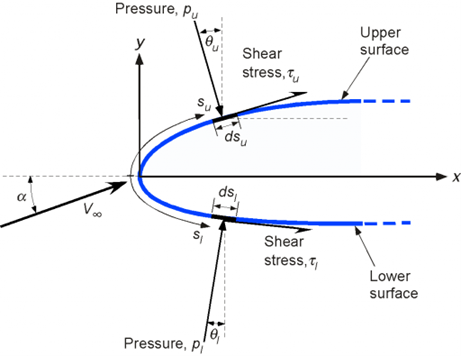
\includegraphics[width=0.8\linewidth]{6DoF Explanation Scripts/Images/ShearStress.png}
    \caption{Pressure and Shear Stress on an Aerodynamic Surface}
    \label{fig:pressure and shear}
\end{figure}

Since a force is a pressure multiplied by an area, $F=pA$, we can integrate our pressure distribution over an area to understand the total forces that are acting on a geometry. Often, we see this expressed in the form of an integral over the length of the geometry. This length is denoted by $c$, the chord length, in the example of the airfoil. These integrals are shown below:
\begin{gather}
    N'=\int_0^{c}{p_lu-p_u}{dx}+\int_0^{c}{\left[\tau_u\frac{dy_u}{dx} + \tau_l\frac{dy_l}{dx}\right]}{dx}\\\\
    A'=\int_0^{c}{\left[p_u\frac{dy_u}{dx} + p_l\frac{dy_l}{dx}\right]}{dx}+\int_0^c{(\tau_u+\tau_l)}{dx}
\end{gather}
Where the $N'$ and $A'$ are the normal and axial force on the aerodynamic surface. Here, the apostrophe (We would say 'N prime') refers to the fact that the force acts over a unit length in the $\hat{z}$ direction. We are assuming a unit length here since we are considering the 2-D case in this example. More generally, we would perform this calculation in 3D, but that is beyond the scope of this example.

The normal force acts normal in the $\hat{y}$ direction and the axial force acts in the $\hat {x}$ direction as shown in Figure \ref{fig:pressure and shear}. Normal and axial forces are not commonly used in our modeling outside of these calculations. More often, we see the quantities lift and drag, which are defined with respect to the \gls{freestream} velocity. We can easily transform our normal and axial forces into a lift and drag using a rotation matrix with our \gls{angle of attack}, $\alpha$. This rotation matrix takes the form:
\begin{equation}\label{eq:LDMatrix}
 \begin{bmatrix}
     D'\\L'
 \end{bmatrix}
 =\begin{bmatrix}
        \cos\alpha &\sin\alpha\\
        -\sin\alpha&\cos\alpha
    \end{bmatrix}
    \begin{bmatrix}
        A'\\N'
    \end{bmatrix}
\end{equation}
We can expand \eqref{eq:LDMatrix} to give two scalar equations:
\begin{gather}
        L'=N'\cos\alpha-A'\sin\alpha\\
        D'=A'\cos\alpha+N'\sin\alpha
\end{gather}
So, if we know the distribution of pressure over our body, we have shown that we can find the resultant aerodynamic forces acting on our body. As briefly described in Section \ref{sec:moments}, another important parameter to find is our center of pressure.
\subsection{Center of Pressure}
Simply stated, the center of pressure is the location at which all the aerodynamic forces acting on a body produce no resultant moment. This location is particularly useful for our case because we can assume that the lift and drag forces act through the center of pressure rather than assuming that lift and drag act as force distributions. This will make our future calculations much simpler, so we would like to know the center of pressure and how to calculate it.

To find the location where the center of pressure occurs, we can take the moment about any point first. Often, we choose to take the moment about the nose of the rocket (called the leading edge when referring to a wing), since we define the origin here. This integral has a similar form to the normal and axial force integrals except that we multiply the force by the distance from the nose. For more information on why this is done, refer to \cite{gundersen_understanding_2020}. Writing out this integral, we get:
\begin{gather}
    M_{LE}'=\int_0^c{p_u-p_l}{dx}+\int_0^c{\left(\tau_u\frac{dy_u}{dx}+\tau_l\frac{dy_l}{dx}\right)}{xdx}\\+\int_0^c{\left(p_u\frac{dy_u}{dx}+\tau_u\right)}{y_udx}+\int_0^c{\left(-p_l\frac{dy_l}{dx}+\tau_l\right)}{y_ldx}
\end{gather}
Knowing the normal force and the moment about the leading edge, we can find the center of pressure location as:
\begin{gather}
    \color{blue}\boxed{\color{black}x_{cp}=\frac{-M_{LE}'}{N'}}
\end{gather}
We note that the convention for the moment about the nose is for a positive moment to denote a pitch up (this is why the negative sign is present). This is opposite the convention established by the \gls{rhr}. For all other moments used in our 6-\gls{dof} models, we use the standard \gls{rhr} convention for moments.

For more information on the derivation of the equations in this section, refer to Chapters 1 and 2 of \cite{anderson_fundamentals_2017}.

For a rocket, we generally consider the body to be \textit{axisymmetric} about the longitudinal axis, when the whole structure can be rotated about the axis which we define as $\hat{X}$. 

Because our rocket is axisymmetric, we assume that the center of pressure always lies along the longitudinal axis. Although this assumption is not necessarily true, as we will see later, the largest effects on the aerodynamic moments will occur from changes along the longitudinal direction rather than changes along the \textit{transverse plane. }We can think of this intuitively because of the center of pressure is separated from the center of mass by more than the diameter of the rocket, so changes in this direction have a greater effect.
\section{Atmospheric Modeling}
Another hurdle to overcome when describing the aerodynamics of our system is to find values for our \gls{freestream} quantities. We explore the calculation of $V_{\infty}$ in Section \ref{sec: Newtonian Dynamics}. The other parameters we need to calculate are $\rho_{\infty}$ and $a_{\infty}$. Fortunately, the standard density and Mach number of the atmosphere on Earth is well defined. In MATLAB, we can find this density at any altitude with "atmosisa" as:
\begin{lstlisting}[style=Matlab-editor]
    [T, a, P, rho] = atmosisa(height);
\end{lstlisting}
This gives us a standard value of $\rho_{\infty}$ and $a_{\infty}$ to use. However, the value of can vary by up to 10\% depending on the weather conditions \cite{svickova_air_2020}. Similarly, the Mach number has a strong dependence on temperature $\left(M=\sqrt{\gamma RT}\right)$, so the free-stream Mach number may also be different by 10-20\% of standard values. 

All of this is to say that using "atmosisa" gives us a good baseline model of the atmosphere, but is not the final say in atmospheric modeling. For now, we use "atmosisa" in our modeling because we can live with this variation in our model. However, it may be useful in the future to use other sources of atmospheric data that give location- and time-specific data.
\section{Computational Aerodynamics}
In the case of our rocket, we encounter a variety of flight regimes from subsonic to high supersonic. Because of this variety, hand calculations of our aerodynamics can become very complicated. As a result, we choose to use computational tools to compute the aerodynamics of our rocket.
\subsection{RasAero}
The main tool that we use presently is RasAero. This tool allows us to input the geometry of the rocket and will output the drag coefficient as a function of the Mach number. This is less than perfect, as we lose some of the dependence on Reynolds number. Additionally, the dependence on angle of attack is quite course (only measurements every 2$\degree$. That being said, RasAero has been used to model many rocket systems around the same scale as our rocket with an average error in apogee of $3.47\%$ and $80\%$ of the flights within $\pm10\%$ of the true apogee. For us, this is an acceptable compromise so that we can focus on flight dynamics modeling rather than aerodynamics.

More information on RasAero can be found at \cite{rogers_rasaero_2019}. The documentation on this page does a better job explaining the software than we could here in a short summary. Our implementation uses the .csv export files from RasAero in MATLAB.
\subsection{Other Computational Models}
\newacronym{cfd}{CFD}{Computational Fluid Dynamics}
It is worth noting that other computational models exist. RasAero does have shortcomings in modeling some of the aspects of the rocket geometry, so other methods such as \gls{cfd} are also options to be explored. However, in the current state of our model, we have not looked into \gls{cfd} methods very heavily for direct use in MATLAB. These are in the preliminary stages of investigation and will likely be explored more heavily in future editions of this text.

% \section{Wind Modeling}
% Add our wind modelling stuff here (might actually want to model wind first lmao)
\section{Key Ideas}
\begin{enumerate}
    \item When we model a system such as our rocket, we can capture most of the phenomena by capturing data at different $Re$, $M$, and $\alpha$. This is true for both \gls{cfd} and wind tunnel modeling.
    \item While exact analytical solutions are hard to attain in aerodynamics, we can use computational tools to estimate aerodynamics
\end{enumerate}

\section{Further Reading}

There are many good resources for aerodynamics modeling. The first among these, which serves as a good introduction to the topic of fluid dynamics, is \cite{anderson_fundamentals_2017}.

For more complex studies of aerodynamics, we recommend Modern Compressible Flow by Anderson.

\section{Practice Problems}
\begin{enumerate}
    \item You are flying home one day in your P-51 Mustang. At cruise, your aircraft is 10,000 ft above sea level.
\begin{enumerate}
    \item What is the density of air at this altitude?
    \item Your wings provide a $C_L$ of 0.3 at cruising speed. Your plane has a mass of 4,000 kg and a planform area of $21.8 \mathrm{\ m}^2$. Find the speed necessary to maintain level light at this altitude.
    \item Your airplane is equipped with  unguided HVAR rockets. As a daring pilot, you want to model the aerodynamics of this rocket so you can launch it at your friend's house with astounding accuracy (\textit{that} will teach them to never steal your mini corn dogs).
    
    Using your best engineering judgment of the nose cone shape and any other parameters you cannot find, model the HVAR rocket in RasAero.
    \item As it turns out, shooting rockets at Canadian civilians is illegal (I know, right?). The Royal Canadian Air Force F/A-18's are on your tail now and you will be shot down in 15 minutes unless you can make it to US airspace. You are 160 km from the airspace boundary. You push your throttles to full to book it back home. 

    At full throttle, your Merlin V12 produces 1676 hp (1250 kw). Your aircraft has a $C_D$ of 0.017. At the same altitude of 10,000 ft, find the maximum flight speed. Will you make it back to American airspace in time?

\end{enumerate}
\end{enumerate}
\chapter{Numerical Integration Schemes}\label{sec:numerical integration schemes}

\begin{chapquote}{Wolfgang Pauli}
    ''The best that most of us can hope to achieve in physics is simply to misunderstand at a deeper level.''
\end{chapquote}

In our exploration of numerical integration schemes, it will be useful to have a good understanding of ordinary differential equations. We highly recommend \cite{dawkins_differential_2023} for reviewing differential equations.

We note that this section does not include practice problems since most of the other practice problems include numerical integration as part of the process.

\section{Euler Integration}\label{sec:euler integration}
We have previously discussed the simplest integration scheme, the explicit Euler method, which we used in Section \ref{sec: Numerical Integration in the 1DoF}. Understanding the Euler method is key to understanding and using more complex integration schemes, so we recommend writing a few of your own Euler integration scripts in MATLAB or a coding language of your choice to really solidify your knowledge before moving on to more complex integration schemes. 

We formalize the explicit Euler integration below. Given a linear ODE:
$$\frac{dy}{dt}=f\left(x,y\right)$$
With initial condition:
$$y(x_0)=y_0$$
We perform Euler integration first by defining an interval over which to perform the numerical integration. For Euler integration, we equally space these points by our timestep, $dt$. We can parameterize these points as:
$$x_i=x_0+i\Delta t$$
Our next step is to find the value of the tangent line at each point. This is trivial, since our differential equation tells us what $\frac{dy}{dt}$ looks like at any value. All we have to do is evaluate:
$$\frac{dy}{dt}=f\left(x_i,y(x_i)\right)$$
The problem here is that $y(x_i)$ is an unknown quantity (if we knew it, we wouldn’t have to do integration). So, to find the value of $y(x_i)$ we take an iterative approach. We know the starting value, $y(x_0)=y_0$, so we can find an approximation of the new value by multiplying the timestep by the current slope. For the first timestep, this will look like:
$$y_1=y_0+\Delta t\cdot f(x_0,y_0)$$
Now that we have found an approximation for $y_1$, we can extend this to find approximations for $y_2$, $y_3$, etc. This formula is generally extensible as:
\begin{gather}
    \color{blue}\boxed{\color{black}y_{n+1}=y_i+\Delta t \cdot f(x_i,y_i)}\\
    \color{blue}\mathrm{Euler's \ Method}
\end{gather}

We represent this Euler integration scheme graphically with a simple example. Suppose our differential equation is $\frac{dy}{dt}=2t$ with initial condition $y(0)=0$. In this example, we can see from inspection that the solution curve is $y=t^2$. Performing Euler integration with a $\Delta t$ of 0.5 yields the black approximation in Figure \ref{fig:Euler}.
\begin{figure}[ht]
    \centering
    
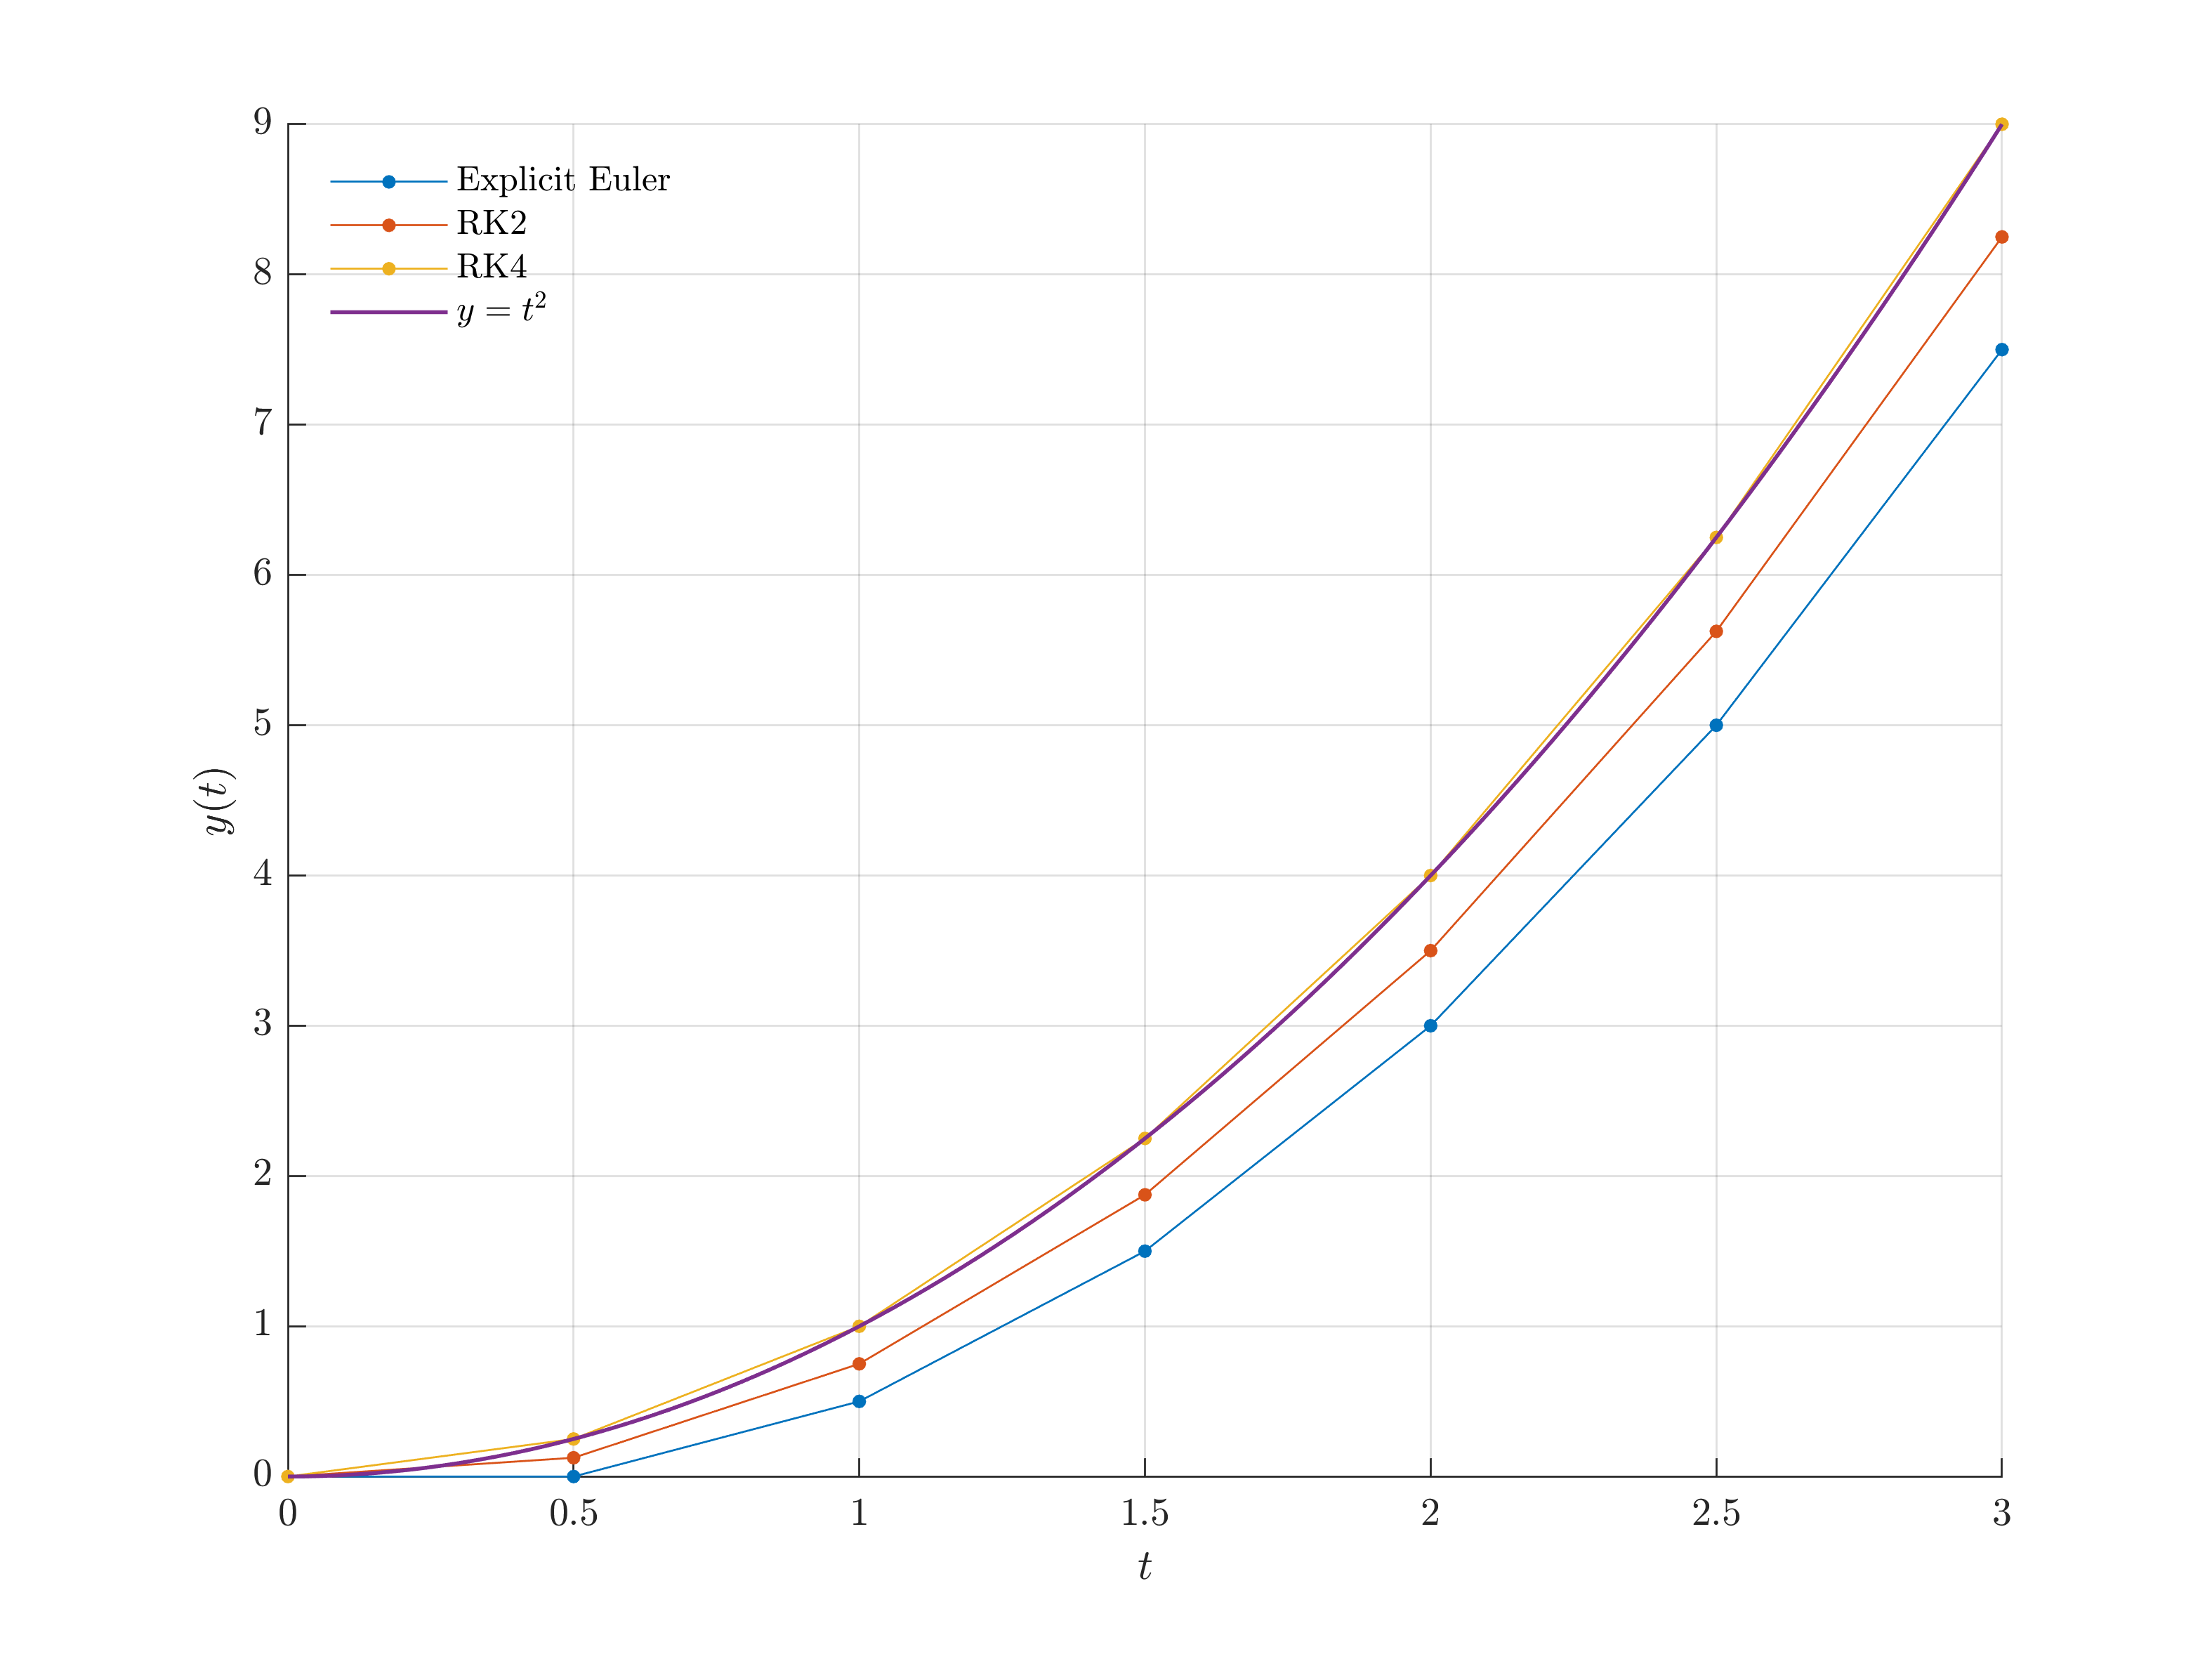
\includegraphics[width=\linewidth]{6DoF Explanation Scripts/Explicit Euler Approximation Figure.png}
    \caption{Explicit Euler Method Numerical Approximation}
    \label{fig:Euler}
\end{figure}

As can be seen from Figure \ref{fig:Euler}, large timesteps quickly lead to error in the solution. For a strictly convex curve, our Euler approximation will always give us an under-approximation of the solution. In some cases, however, our solution may diverge so greatly that it becomes unstable and values tend toward infinity.\footnote{This is especially true for periodic functions. When working with periodic functions, make sure to sample well below the Nyquist limit.}
 
% In Table 2 below, we describe the benefits and drawbacks of Euler integration.

% \begin{table}[ht]
% \begin{tabular}{ll}
% Benefits                                                                                                                                                    & Drawbacks                                                                                                                                                             \\
% \begin{tabular}[c]{@{}l@{}}Simple\\ Good for very quick implementations / testing\\ Robust and easy to implement\\ Good for simple explanation\end{tabular} & \begin{tabular}[c]{@{}l@{}}Less precise than other integrator schemes\\ More prone to solution singularities\\ Generally has fixed timestep calculations\end{tabular}
% \end{tabular}
% \end{table}

\subsection{Errors in the Euler Method}\label{sec:errors in the euler method}
We will use the example of the Euler Method to demonstrate error in numerical integrators. These same concepts will apply when we move on to higher order integrators. 
\newglossaryentry{trunc error}
{
    name=truncation error,
    first = {\textit{truncation error}},
    description={Error in numerical integration that comes from the inaccuracies of the integration scheme in modeling the true behavior of the function. This error is related to the number of higher order terms ignored}
}

\newglossaryentry{roundoff error}
{
    name=roundoff error,
    first = {\textit{roundoff error}},
    description={Error in numerical integration that comes from inaccuracies in the floating point precision of computers. This is worsened by a larger number of timesteps, as this error will compound}
}
Errors in the integration scheme come from two different sources:

1. Euler integration schemes only account for linear terms because it only considers the slope of the tangent line at a point. Thus, any quadratic order terms or higher will not be accounted for. Thus, the error is proportional to the timestep squared, $\Delta t^2$.\footnote{This intuitive explanation is not entirely correct, see (3) for a full derivation using the Taylor Series. We also note that the technically correct way to denote this is $O(\Delta t^2)$, meaning the error is of order $\Delta t^2$} We call this error \gls{trunc error}.

2. Another problem is the fact that computers don’t have infinite precision. The loss of precision during computing is called \gls{roundoff error}. Computing more timesteps in total will increase this \gls{roundoff error}.

It is worth noting that these errors are per timestep! So over the course of a full simulation, our errors will grow much larger than the error bounds that we’ve calculated above. In fact, for the Euler Method described above, the global error is proportional to the timestep, $\Delta t$.

We can of course, reduce errors in the simulation by reducing our timestep, $\Delta t$. However, this will also increase the computation time. Additionally, doing so will increase the \gls{roundoff error} in the simulation. With more calculations being done, the \gls{roundoff error} will have a larger impact. Thus, it is worthwhile to investigate other integration schemes.

\section{Improved Euler / RK2}
Given the limitations of the Explicit Euler method, we will start by investigating the improved Euler Method. This improved Euler method is the first of a family of integration schemes known as Runge-Kutta (RK) integration schemes. The number, 2, represents the order of the integration scheme, which we will explore more later.

The main area that led to inaccuracies in the explicit Euler method was the slope that we calculated. We can improve on this by taking two points and finding the average slope. We choose to take a point at our start and our end point, $x_i$ and $x_{i+1}$, and evaluate the slope at both of those points and average them. From the previous section, we can remember that:
\begin{equation}
    \frac{dy}{dt}=f\left(x_i,y(x_i)\right)
\end{equation}
So, we can write the average slope as
\begin{equation}
    m=\frac{\dot{y}_1+\dot{y}_2}{2}
\end{equation}
Where
\begin{gather}
    \dot{y}_1=\frac{dy_1}{dt}=f\left(x_i,y(x_i)\right)\\
    \dot{y}_2=\frac{dy_2}{dt}=f\left(x_{i+1},y(x_{i+1})\right)
\end{gather}
Now that we have the slope, we follow the same process as we did for the Explicit Euler method to find the next value. We take the slope and multiply it by the timestep, $\Delta t$, and add the current value, $y(x_i)$. This gives us our approximation as:
\begin{equation}
    y=y(x_i)+\frac{\dot{y}_1+\dot{y}_2}{2}\Delta t
\end{equation}
We can write this then as:
\begin{equation}
    y_{i+1}=y_i+\frac{\Delta t}{2}\left[f(x_i,y(x_i))+f(x_{i+1},y(x_{i+1}))\right]
\end{equation}
To rewrite this equation in a way that is better suited for code:
\begin{gather}\label{eq:rk2}
    y_{i+1}=y_i+\frac{\Delta t}{2}(k_1+k_2)\\\\
    k_1=f(x_i,y_i)\\
    k_2=f(x+\Delta t, y_i+\Delta tk_1)
\end{gather}
We can note here that this method requires at least two evaluations since $k_2$ is dependent on $k_1$. However, this is often still more computationally efficient than the Explicit Euler method because larger time steps can be used with lesser error.

\subsection{RK2 in Code}
\newglossaryentry{func handle}
{
    name=function handle,
    first = {\textit{function handle}},
    description={A pointer to an instance of a function in MATLAB. A function handle essentially stores a function call in a variable in MATLAB.}
}
Implementing the RK2 algorithm in code is slightly more complicated than implementing the explicit Euler method. To properly implement this, we will use \glspl{func handle} in MATLAB. \Glspl{func handle} act as pointers to an instance of a function. To explain what that means, we will examine the following code snippet:
\begin{lstlisting}[style=Matlab-editor]
f = @computeSquare;
a = 4;
b = f(a)
\end{lstlisting}
where "computeSquare" is defined as:
\lstset{style=mystyle}
\begin{lstlisting}[style=Matlab-editor]
function y = computeSquare(x)
y = x.^2;
end
\end{lstlisting}
The \gls{func handle} allows us to assign the function to a variable, which we are calling "f". We call this a pointer because this variable ‘points’ to the function "computeSquare".

In this example, when we call this operation, we get "b=16" in the command window. The power of this is that we could instead pass in a vector of values for "a" and get outputs from the function for all of them. If we instead input:
\begin{lstlisting}[style=Matlab-editor]
f = @computeSquare;
a = [4,6,10];
b = f(a)
\end{lstlisting}
We get an output of "b = 16  36  100". The usefulness of this is immediately apparent for numerical integration. We can pass in a vector of many different times and get outputs for each of them. 

Another useful feature of \glspl{func handle} for numerical integration is that they allow us to pass in only the variables needed for numerical integration and pass other variables in the expression as constants. In general, we want our numerical scheme to only accept our \gls{state vector} and the time vector. This is the same thing that "ode45" does, so it is best practice to do the same thing here.

Our RK2 algorithm is a direct translation of \eqref{eq:rk2} into code. We present this below in Listing \ref{code:rk2}:
\begin{lstlisting}[style=Matlab-editor, caption=RK2 Integrator]
%% RK2 Integrator
% numerically integrates a first order initial value problem using Runge-Kutta 2nd order.
% inputs:
% fun - function of integration
% dt - time step [s]
% tIn - input time [s]
% xIn - initial value input vector
% outputs:
% out - final value output vector
function out = rk2(fun, dt, tIn, xIn)
    f1 = fun(tIn,xIn);
    f2 = fun(tIn + dt/2, xIn + dt .* f1);
    
    out = xIn + (dt / 2)*(f1 + f2);
end
\end{lstlisting}\label{code:rk2}
%% add more on making functions and rk2.

\section{RK4 Integration}\label{sec: rk4}
RK4 integration is the last major integration scheme that we will explore. RK4 integration is often the best balance between the precision of the algorithm and the speed of computation. 

To explain the RK4, we will go back to the RK2 and explain it in a slightly different way that will shed light on what we are doing with RK4. In RK2, we described taking the average slope of the function. We can also imagine taking the Taylor expansion of our function:
$$y_{i+1}=y_i+\dot{y}_i\Delta t+\ddot{y}_i\frac{\Delta t}{2}+O\left(\Delta t^3\right)$$
From this Taylor expansion of the solution, we can that our approximation accounts for linear and quadratic terms. Thus, our error is proportional to terms to the 3\textsuperscript{rd} power, represented by $O(\Delta t^3)$. We know $y_i$ and $\dot{y}_i$, but the 2nd order derivative of our function is unknown. We can approximate this 2nd order derivative as:
$$y_i=\frac{\dot{y}_{i+1}-\dot{y}_i}{\Delta t}$$
Upon rearranging this equation, we can see that we arrive at the same expression as we did before. We can apply the same approach for the RK4 integration, except we consider terms up to the 4\textsuperscript{th} order expansion of the Taylor series:
$$y_{i+1}=y_i+\dot{y}_i\Delta t+\ddot{y}_i\frac{\Delta t}{2}+\dddot{y}_i\frac{\Delta t}{6}+\ddddot{y}_i\frac{\Delta t}{24}O\left(\Delta t^5\right)$$
Immediately, we can see that our error has shrunk to be proportional to terms of the 5\textsuperscript{th} order, a dramatic reduction as compared to RK2 or Explicit Euler method.

\subsection{RK4 Integration in Code}
The RK4 Integration scheme can be expressed as a set of equations very similar to what we did with \eqref{eq:rk2}. We will not derive these equations here, because the process is very similar to that used for the RK2 method.

The form of these equations is shown in \eqref{eq:RK4}.
\begin{gather}\label{eq:RK4}
    y_{i+1}=y_i+\frac{\Delta t}{6}\left(k_1+2k_2+2k_3+k_4\right)\\\\
    k_1=f(x_i,y_i)\\
    k_2=\left(x_i+\frac{\Delta t}{2},y_i+\frac{\Delta t}{2}k_1\right)\\
    k_3=\left(x_i+\frac{\Delta t}{2},y_i+\frac{\Delta t}{2}k_2\right)\\
    k_4=f(x_i+\Delta t,y_i+\Delta tk_3)
\end{gather}
An implementation of this algorithm into code is shown below.
\begin{lstlisting}[style=Matlab-editor, caption=RK4 Integrator]
%% RK4 Integrator
% numerically integrates a first order initial value problem
% inputs:
% fun - function of integration
% dt - time step [s]
% tIn - input time [s]
% xIn - initial value input vector
% outputs:
% out - final value output vector
function out = rk4(fun, dt, tIn, xIn)
    f1 = fun(tIn,xIn);
    f2 = fun(tIn + dt/2, xIn + (dt/2) .* f1);
    f3 = fun(tIn + dt/2, xIn + (dt/2) .* f2);
    f4 = fun(tIn + dt, xIn + dt*f3);
    
    out = xIn + (dt / 6)*(f1 + 2*f2 + 2*f3+f4);
end
\end{lstlisting}\label{code:rk4}
Often, we use a function in MATLAB called "ode45" to perform RK4 integration. This function has the benefit that it will change the step size to produce high accuracy when needed and decrease computation time otherwise.

An understanding of the operation of "ode45" is best motivated by an example. We include an example of a Lorenz Attractor in the Appendix \ref{sec:Lorenz Attractor RK4 Example} as an example of ode45. We recommend reading through this code and running it, as well as changing parameters to see how it affects the outputs.
\subsection{ODE45 Usage}
While examples are helpful, it is useful to see the inner workings of "ode45" for a new user. 

"ode45" relies on the function handles that we mentioned earlier. "ode45" takes as inputs the integration function, time span, and initial state vector.

"ode45" only takes integration functions that are a function of time and the state variable, or "(t,x)" in MATLAB notation. If we have an integration function that is a function of more than just these two variables, we need to pass them through using function handles. We can do this in the following manner:

\begin{lstlisting}[language=Matlab]
@(t,x) integrator(t,x,a,b)
\end{lstlisting}
In this example, we have a function that performs our numerical integration, called "integrator", the output of which will be the derivative of our state vector. We want "ode45" to see this function and only input "(t,x)", so we put that in a function handle at the front. After the function handle, we are free to pass in any other variables, such as "a" and "b". These will simply be read in as constants in the "ode45" integration scheme.

The benefit of adding these in as a function pass through instead of being computed in "ode45" will become apparent when we discuss code optimization in Section \ref{sec: code optimization}. This also keeps our code hierarchy cleaner and more easily modifiable.

\section{Other Numerical Integration Considerations}\label{sec:other numerical ints}
\subsection{More on Error}
We briefly discuss the error of the integration schemes in each of the previous sections. However, it is useful to see examples of these to solidify understanding. 

Using the same example differential equation from Section \ref{sec:errors in the euler method} as $\frac{dy}{dt}=2t$, we can show the approximation for Explicit Euler, RK2, and RK4. This is shown in Figure \ref{fig:Numerical Comparison}.
\begin{figure}[ht]
    \centering
    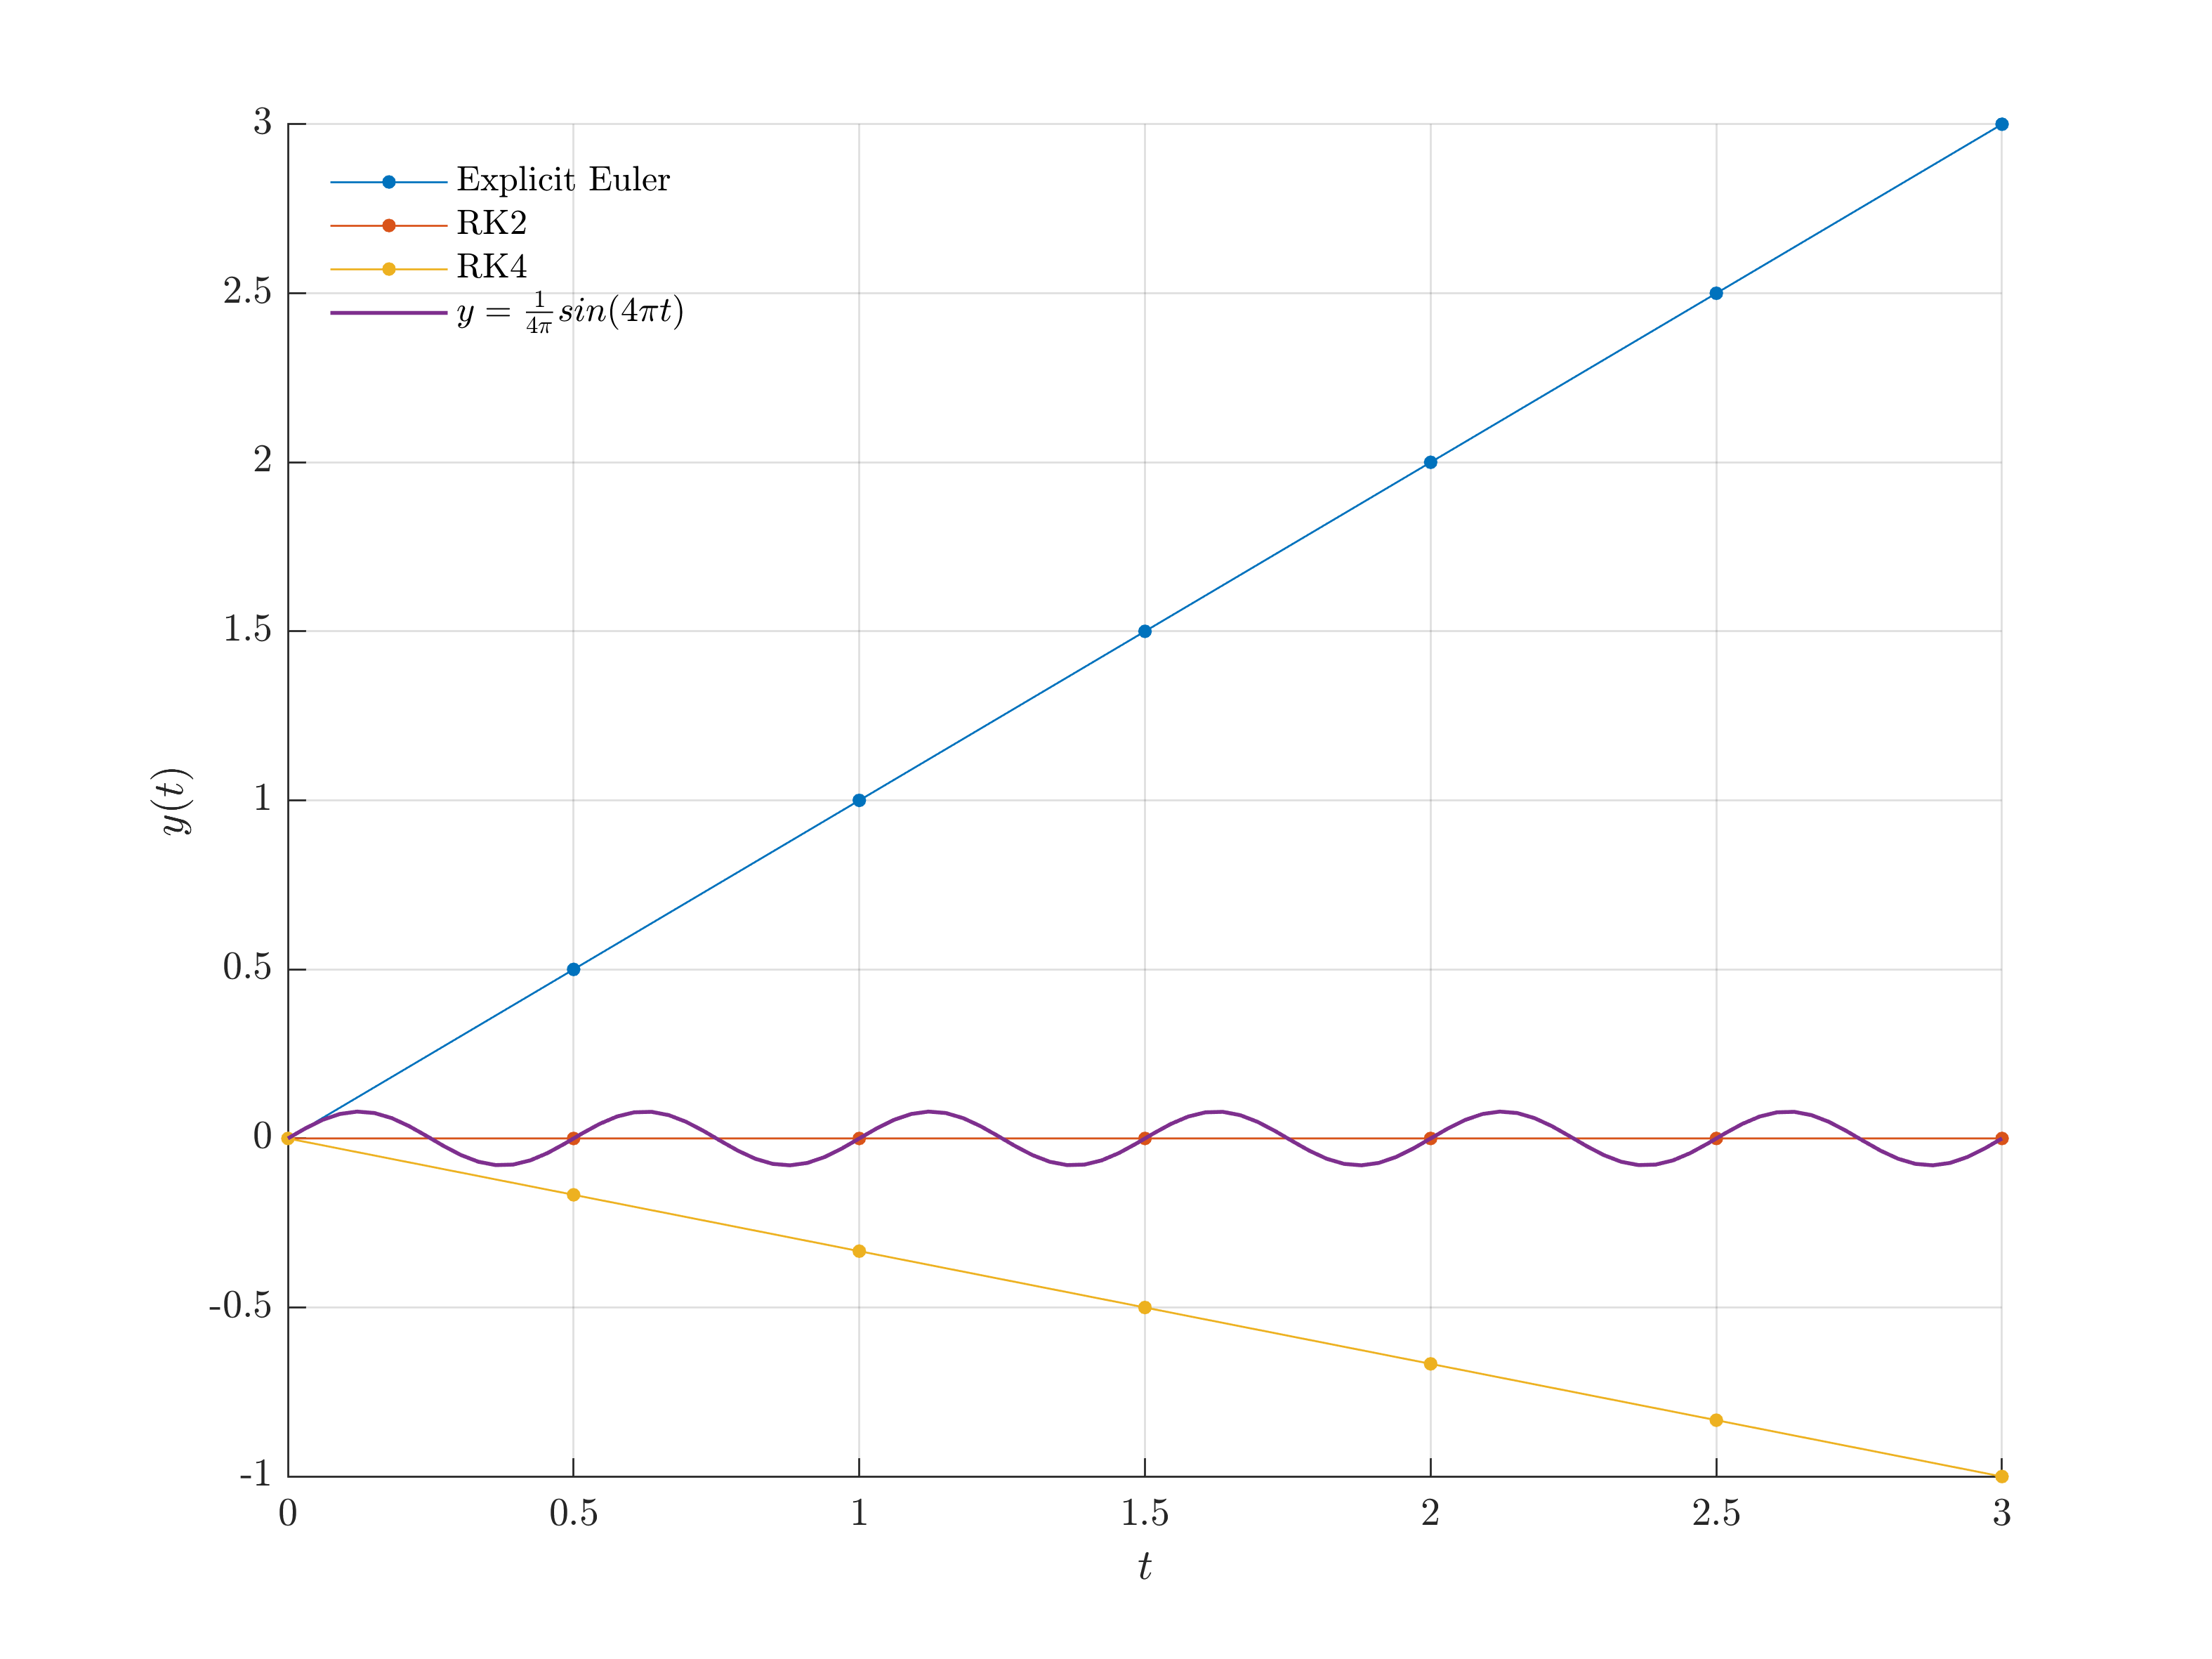
\includegraphics[width=\linewidth]{6DoF Explanation Scripts/Numerical Integrator Comparison Figure.png}
    \caption{Comparison of Numerical Integration Schemes for $y'=2t$}
    \label{fig:Numerical Comparison}
\end{figure}
The code that runs this example is shown in Listing \ref{code:Numerical Error $y'=2t$} in the Appendix. This code is a good example for understanding the syntax for using the integration code snippets in Listing \ref{code:rk2} and Listing \ref{code:rk4}.

As we can see from this example, even with a fairly large timestep of $\Delta t=0.5s$, the RK4 perfectly matches the true curve. For this curve, there are no terms of higher order than quadratic, so the RK4 will perfectly match the solution curve.

The difference in these numerical integration schemes will become more apparent when modeling the behavior of different differential equation systems. Systems containing higher order terms will be better modeled by the higher order integration schemes, unsurprisingly. The true use of these methods is when analytical solutions to the differential equations are hard or impossible to obtain. That being said, we still want to know characteristics of our system so we can appropriately select integration parameters.

\subsection{Sampling and Stiffness}\label{sampling and stiffness}
 To begin our discussion of sampling and stiffness, we can take the differential equation $\frac{dy}{dt}=\cos(4\pi t)$with the initial condition of $y(0)=0$. This function is periodic in nature, so it will be good for our demonstration here. In this first example, we will keep the same timestep of $\Delta t=0.5s$. As is seen in Figure \ref{fig:Numerical Int Periodic}, this timestep is the same as the period of the sinusoidal solution of this differential equation. When this is the case, we can see that the solutions diverge from the original periodic function greatly for all of the integration schemes (aside from the RK2, although this is only the case when the period is exactly the same as the timestep). This occurs because we are not sampling the function at a high enough frequency to capture the nature of the periodic function.

\begin{figure} [ht]
    \centering
    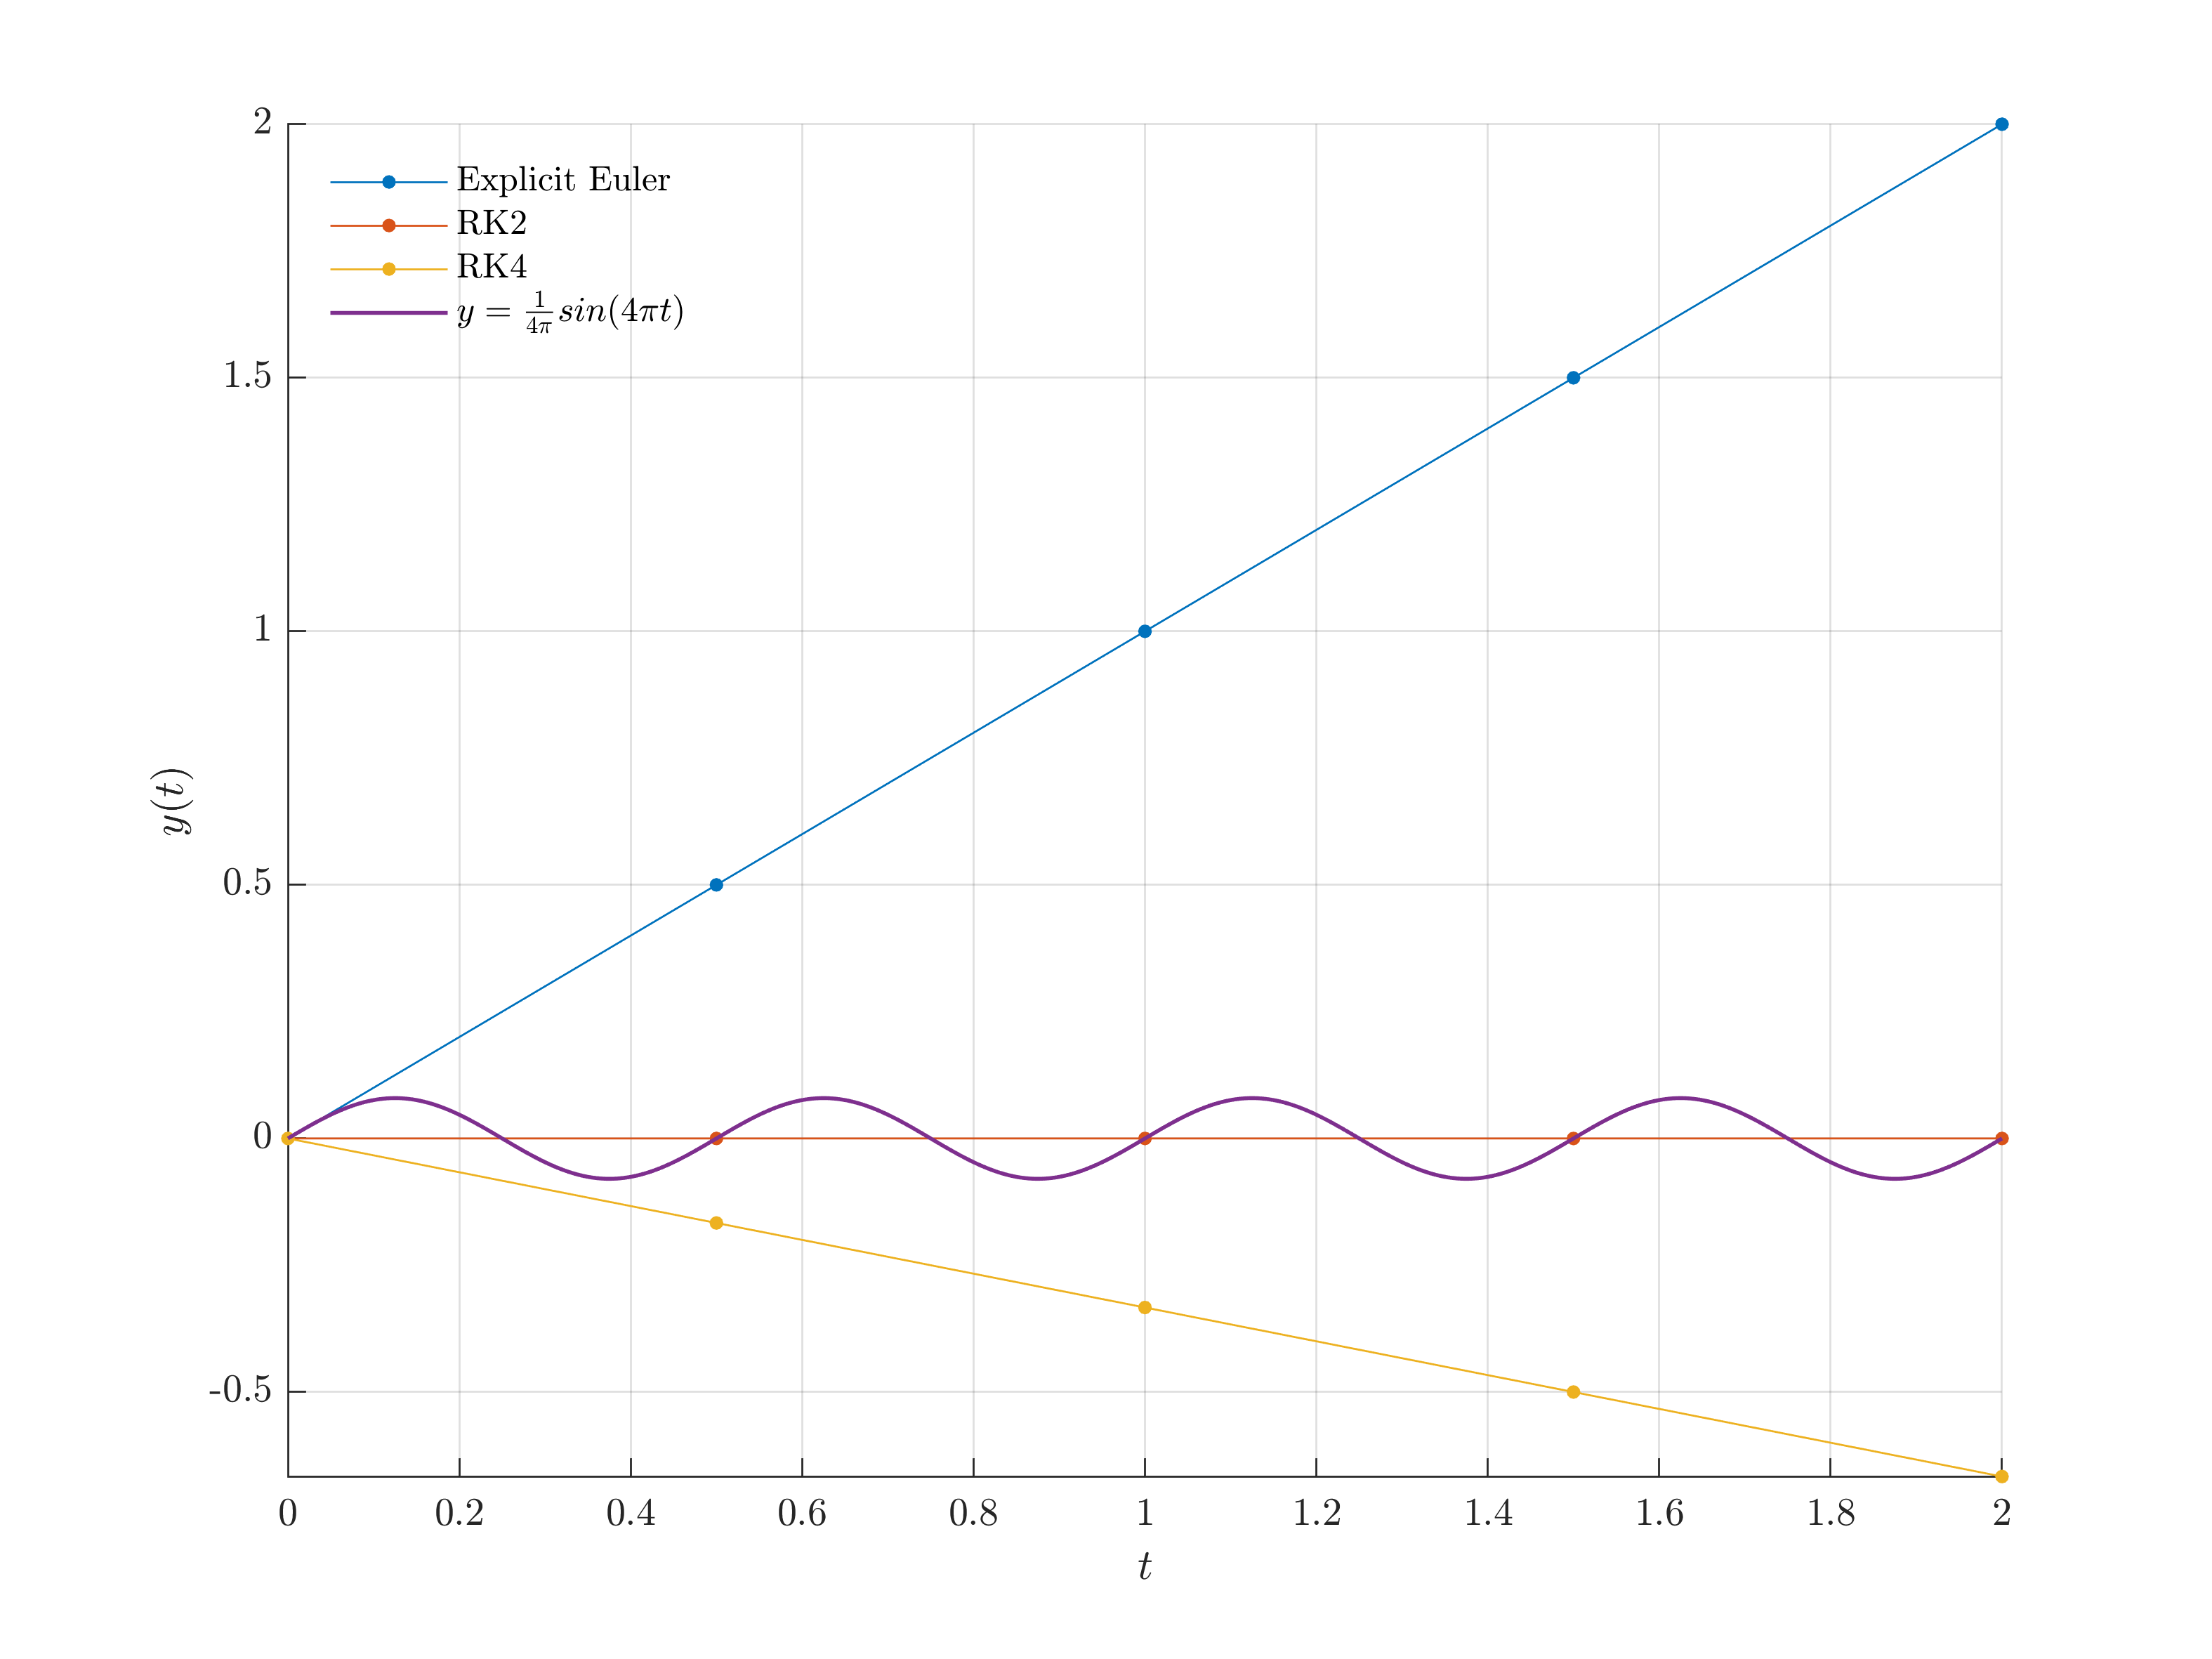
\includegraphics[width=\linewidth]{6DoF Explanation Scripts/Numerical Integrator Nyquist 1.png}
    \caption{Numerical Integration of periodic function}
    \label{fig:Numerical Int Periodic}
\end{figure}
So, what timestep is required to accurately model a periodic function? For our example, we will use RK4 since we have shown it to be the most accurate of the integration schemes. We choose to do this to highlight effects aside from error in the numerical approximation. We can vary the timestep for this same periodic function and see what the response looks like. This is shown in Figure \ref{fig:Nyquist}.
\begin{figure}[ht]
    \centering
    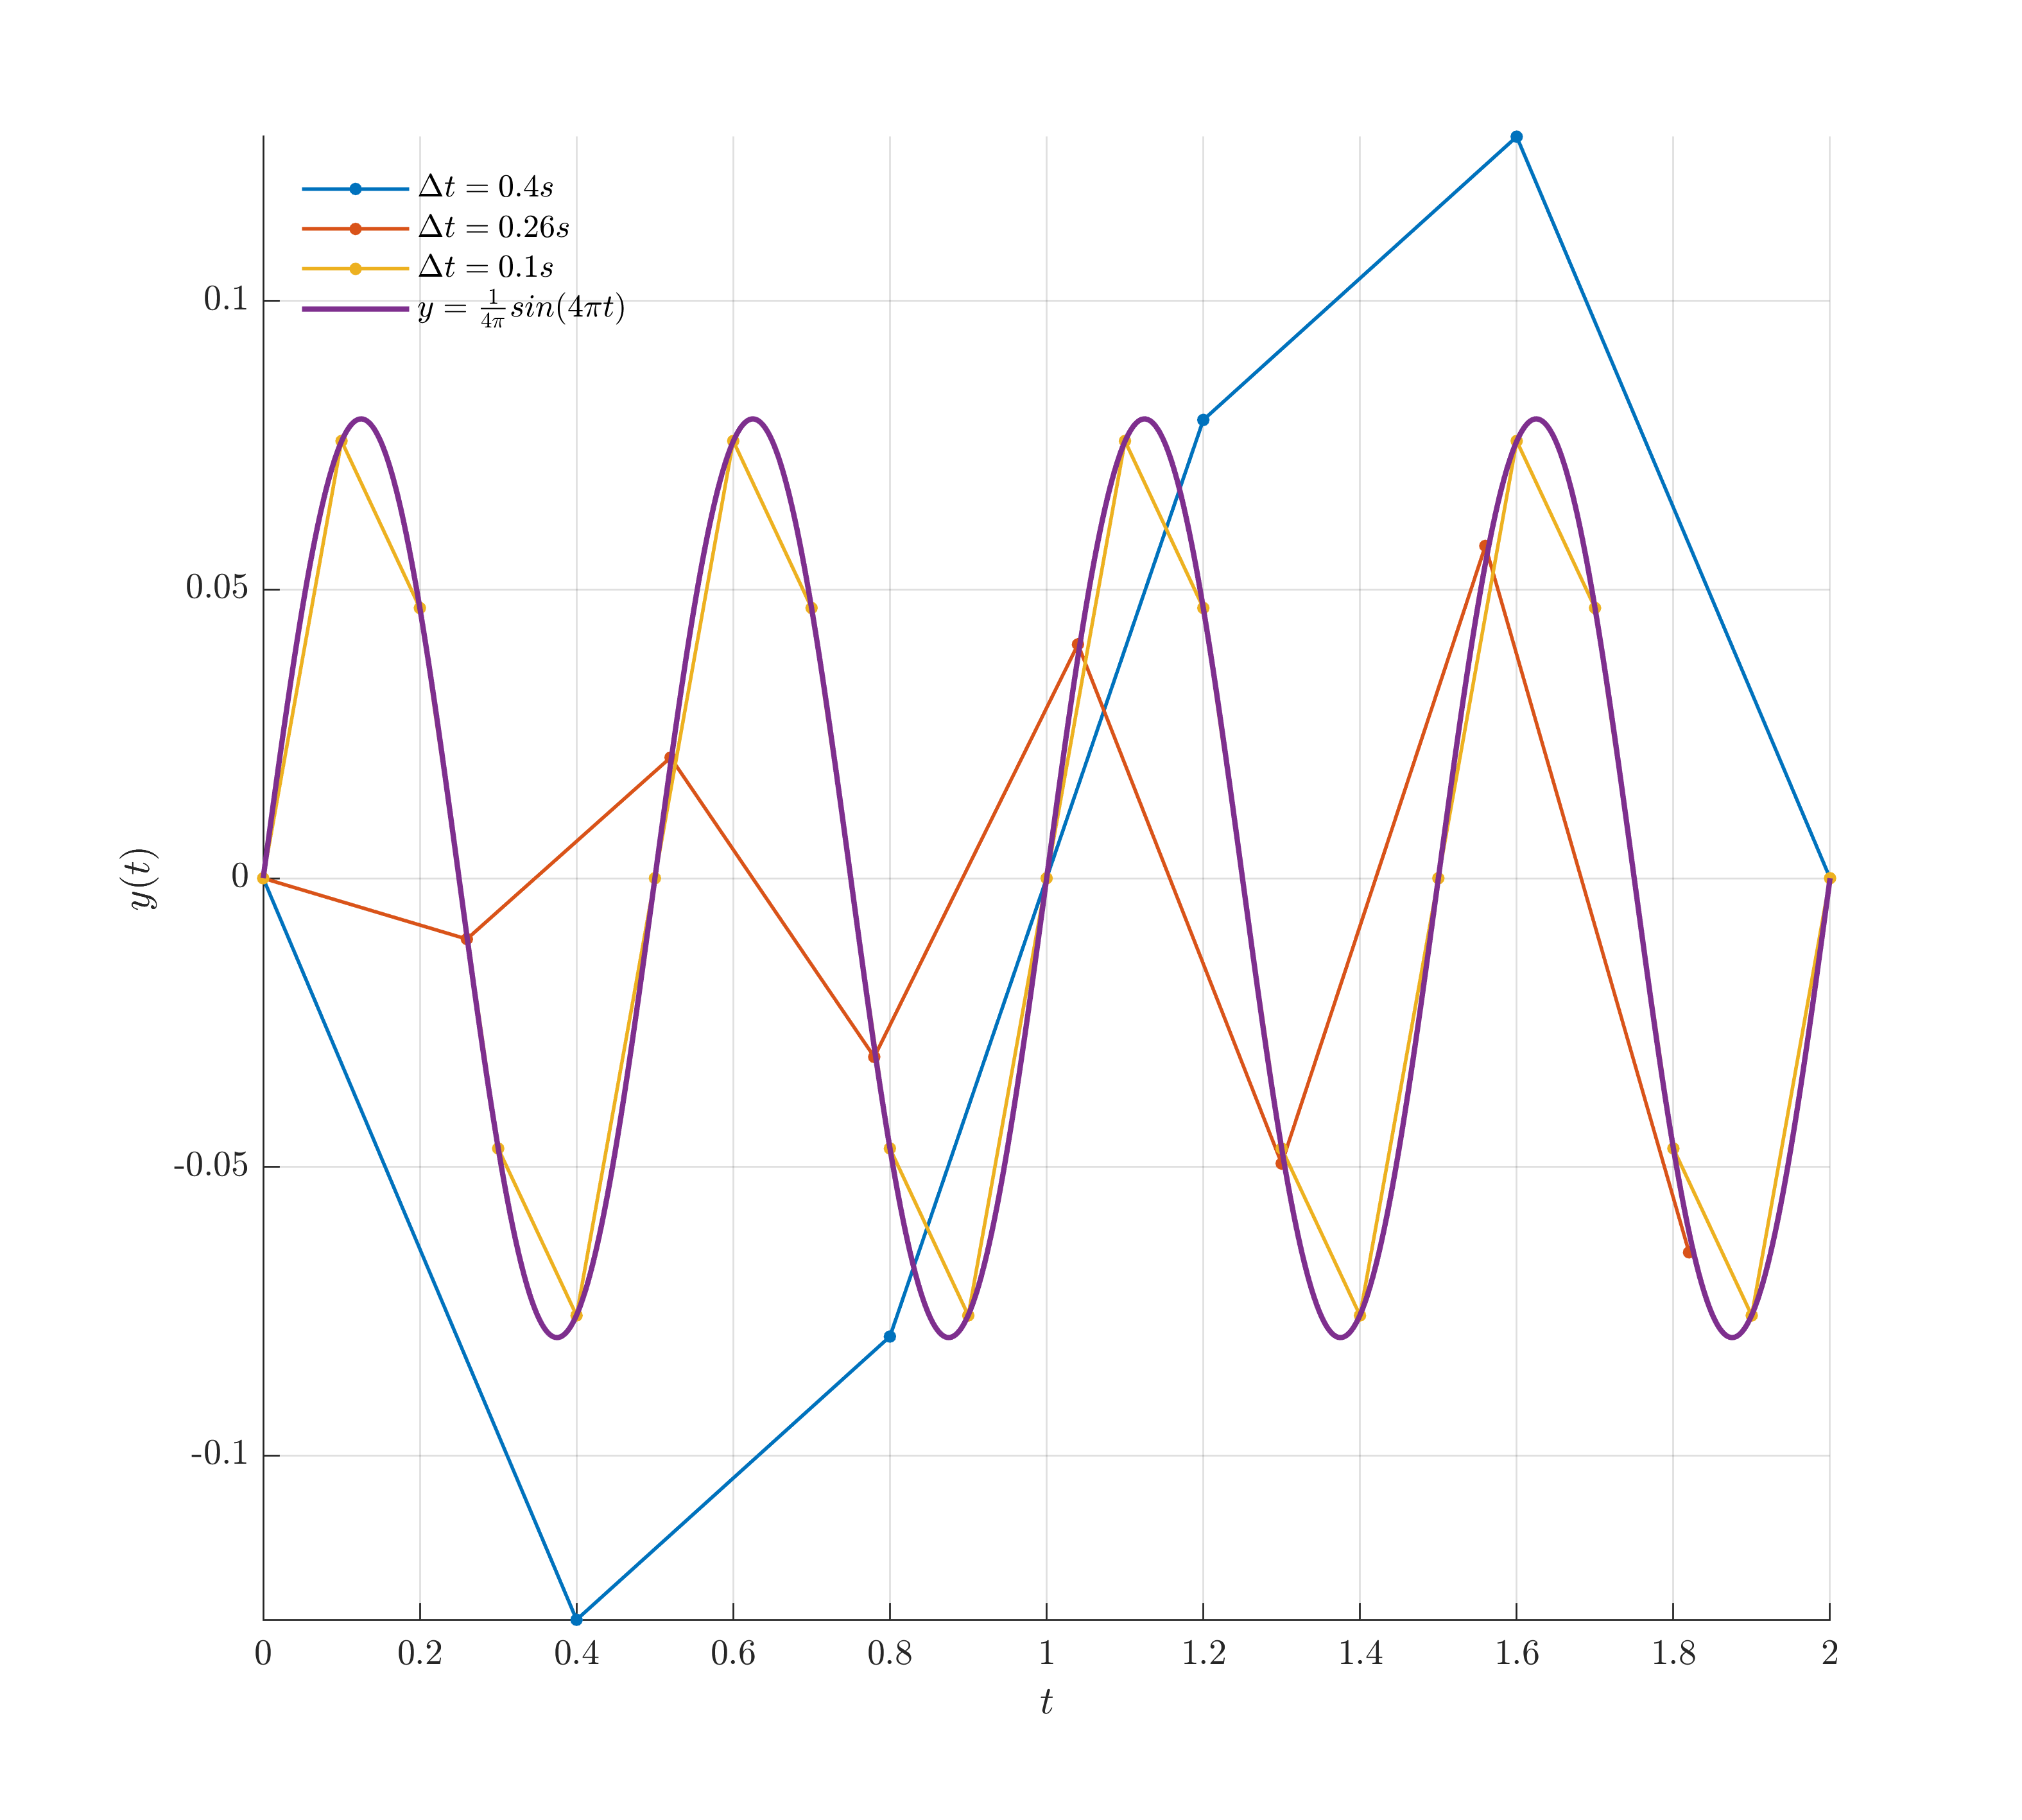
\includegraphics[width=0.9\linewidth]{6DoF Explanation Scripts/Numerical Integrator Nyquist 2.png}
    
    \caption{Numerical Integration of Periodic Function with varying timestep}
    \label{fig:Nyquist}
\end{figure}

\newglossaryentry{beat freq}
{
    name=beat frequency,
    first = {\textit{beat frequency}},
    description={A beat frequency is the result of constructive and destructive interference between two waves of a similar frequency. The similarity of the frequencies creates variations in the amplitude of the resultant wave.}
}

In this figure, we note several important things. When our timestep is slightly less than the period of the function, we infer a lower frequency. This is seen when we use a timestep of $\Delta t=0.4s$. We can intuitively explain this as a \gls{beat freq}. We know that the solution curve has a frequency of 2 Hz, and a wave with a period of $0.4 s$ would have a frequency of 2.5 Hz. Thus, a beat frequency of 0.5 Hz would be produced. This is exactly what is seen, as the resultant solution appears as a sine wave with a frequency of 0.5 Hz (2 second period). 

\newglossaryentry{bandwidth}
{
    name=bandwidth,
    first = {\textit{bandwidth}},
    description={The bandwidth of a signal is the difference between its upper and lower frequencies. In our context of numerical integration, this bandwidth refers to twice the highest frequency of a function}
}

\newglossaryentry{nyquist rate}
{
    name=Nyquist rate,
    first = {\textit{Nyquist rate}},
    description={The rate at which a signal must be sampled to be free of distortions and aliasing. This rate is typically twice the highest frequency present in the signal}
}

The same is seen when $\Delta t$ is close to but not quite double the frequency of the wave (called \gls{bandwidth} of the signal). The perceived signal has a changing amplitude with a superimposed sinusoid. This again, does not match the true signal. It is only when we sample at the \gls{nyquist rate} that a true approximation of the function is found. In general, we must sample our function at twice the highest frequency present to ensure a good approximation!

\newglossaryentry{stiff}
{
    name=stiff,
    first = {\textit{stiff}},
    description={A differential equation that is hard to numerically integrate as a result of instability when larger timesteps are used. Stiffness is a property of the differential equation itself, and not the solution. Stiff systems are not completely well defined, but generally follow from this definition}
}

In this example, this criterion does not greatly affect our numerical integration. However, when we have other dynamics in the system, the need to sample at double the highest frequency of the system may be detrimental to the performance of our simulation. We call such systems that are difficult to numerically integrate \gls{stiff}. 

\Gls{stiff} systems make numerical integration challenging not only because of increased simulation time, but also because of aforementioned \gls{trunc error}. In a 6-\gls{dof} model such as ours, this is important if vibrational modeling is considered. As an example, slosh modeling and parachute modeling (which are not deeply discussed here, but may be important aspects of a rocket 6-\gls{dof}) are often based on mass-spring-damper systems.

It is best practice to try and decouple the simulation of high-frequency vibrations from the flight dynamics of the system. Sometimes this may be unavoidable, such as aircraft with large amounts of wing flexure where aerodynamics and elastic deformation are heavily coupled. However, this should be attempted whenever possible. This problem is very complicated and is the subject of much ongoing research! More information about such dynamics can be found in \cite{shyy_recent_2010}.
\section{Other Integration Schemes}
While "ode45" works very well for most use cases with numerical integration, there are cases where other integration schemes should be considered. We will mainly discuss the implementations that exist in MATLAB. More information about such systems can be found at \cite{mathworks_choose_2024} and \cite{mathworks_summary_2024}.

We previously discuss the concept of \gls{stiff} systems in Section \ref{sampling and stiffness}. 

For systems that have moderate stiffness, we can use "ode23" instead of the more typical "ode45" in MATLAB. Using a lower order integration leads to more course results, but it also allows very stiff parts of the system to be computed faster.

On the converse side, for systems that require very high precision, such as orbits, algorithms of the 8th or 9th order are often used. In MATLAB, such algorithms are used in the "ode78" and "ode89" functions. Using a higher order, the truncation error can be significantly reduced and fewer timesteps are needed when very high tolerances are required. However, in most scenarios, there algorithms are about 300-500\% slower than "ode45" while providing few accuracy benefits. Thus, these algorithms are mostly used for only very high precision use cases.

\subsection{Symplectic and Variational Integrators}
In addition to these numerical integration schemes, there are a variety of integration schemes that use energy conservation as the basis of their integration schemes. These types of integrators are called \textit{symplectic}. These types of integrators directly solve Hamilton's equations for a Hamiltonian system. The form of these equations is discussed briefly 

\section{Numerical Integration Code Optimization}\label{sec: code optimization}
\subsection{Monte Carlo Simulation}
Often, we want to run many simulations with various parameters to gain a better understanding of our system. We call this method of running many simulations the \textit{Monte Carlo} method. Using the Monte Carlo method, we can ascertain information about the likelihood of certain events or approximate quantities that are hard to find analytically by running a large number of simulations and performing statistical analysis on the results. In this document, we will not dive into the methods of statistical analysis and the best ways to perform Monte Carlo simulations. This topic is very deep and is the focus of many peoples’ whole careers.

However, even with only rudimentary analysis, Monte Carlo can prove very useful. We will use the example of Monte Carlo to motivate the need for fast simulations. Often, we run upwards of 1000 simulations and fast computation is necessary to perform this large number of simulations. In this section, we will dive into the various methods to optimize MATLAB code and best practices for flight dynamics.
\subsection{Array and Function Optimizations}
MATLAB is generally quite computationally efficient at computing arrays and matrices. After all, MATLAB is ‘MATrix LABoratory’. However, we still need to be mindful of optimizations to our code.

It is best practice to only import what you need for a function or subroutine. For example, if you have wind data for all of the months out of the year, it is desirable to cull that down to the specific month before running the simulation.

Additionally, it is also beneficial for any imported data or long matrices to be passed into a function rather than called inside a function. \textbf{This is especially important inside the numerical integration scheme! }Running "readmatrix" inside of ode45 or whichever other numerical integration scheme you are using can slow down code upwards of 500\% depending on the length of the matrices being read.

Instead, it is best to pass these arrays into the function. Performing "readmatrix" can be slow because it must check if the values are numeric and organize them into tables. By passing only MATLAB arrays, computations are much faster.
\subsection{Flame Graphs for Optimization}
One important method of optimization is the MATLAB profiler. The primary capability of the profiler is the flame graph. An example of the flame graph is shown in Figure \ref{fig:flame1}

\begin{figure}[ht]
    \centering
    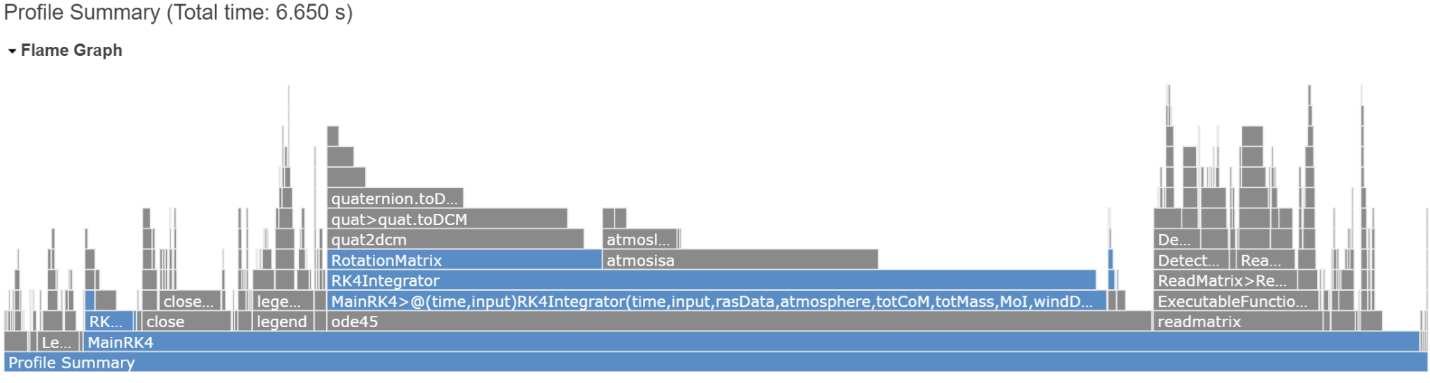
\includegraphics[width=\linewidth]{Images/FlameGraph1.png}
    \caption{Flame Graph Showing Runtime of Individual Code Elements in MATLAB}
    \label{fig:flame1}
\end{figure}

The flame graph gives a visual representation of how long the code spends on each function. Functions in blue are those defined by the user. Those in grey are built in MATLAB functions.

Poorly optimized code will spend a long time running an excessive number of operations. In some cases, this is unavoidable. For example, ode45, which runs the RK4 integration scheme we discussed in Section \ref{sec: rk4}, must run for every time step and is likely to comprise a large part of simulation time.

However, other operations, such as "atmosisa", should not comprise a large portion of simulation time. As seen in Figure 15, calling the atmosisa function on every loop takes about 40\% of the total time spent in ‘RK4Integrator’ function. By instead creating a table of the atmosisa data before running the simulation, we can reduce the runtime quite drastically. Implementing this simple change, we can see the reduction in simulation time as shown in Figure \ref{fig:flame2}

\begin{figure}
    \centering
    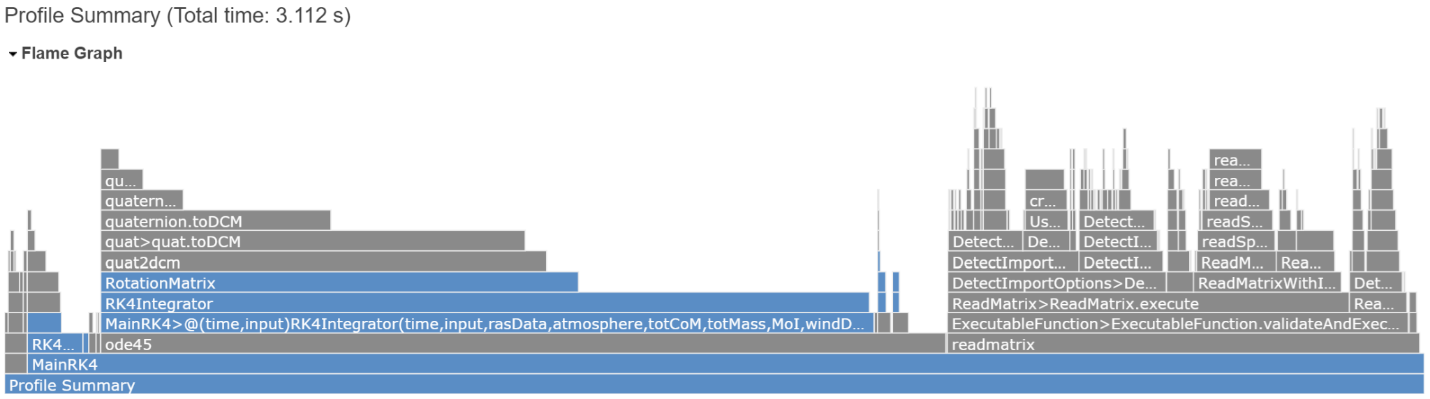
\includegraphics[width=\linewidth]{Images/FlameGraph2.png}
    \caption{Flame Graph After Optimizations}
    \label{fig:flame2}
\end{figure}

\section{Key Ideas}
\begin{enumerate}
    \item Numerical Integration schemes of higher order can better approximate systems. Generally, a higher order will require more up front computation but will be more accurate and will take fewer steps to achieve a given accuracy
    \item When numerically integrating functions with high frequencies or rapid changes, we need to be mindful of stiffness of the system and ensure to sample at at least the bandwidth of the signal.
    \item Keep in mind what you need to calculate inside the integrator and what should be passed through. Calculations inside the integral are very time expensive!
\end{enumerate}

\section{Notes and Further Reading}
For more information and derivations on this section, refer to \cite{trench_31_2020}. This source includes some more information than included here and some useful examples.

The MATLAB documentation for numerical integration schemes is quite good. For non-"ode45" integration, we recoommend the following two documentation sites: \cite{mathworks_choose_2024} and \cite{mathworks_summary_2024}. Other documentation exists within MATLAB for other functions.
%\section{Practice Problems}

\chapter{The 6-DoF}
In this section we will combine everything from the previous sections and explain how our 6-\gls{dof} model works. We will follow a similar set up to Section \ref{sec:Dzhan}  here, describing the elements of the model in detail and then attaching relevant code either in-line or in the appendix.

Our definitions of our frames follow from those discussed in Section\ref{sec:Frame of Reference}. For the earth-centered inertial frame, we follow the conventions discussed in Figure \ref{fig:InertialFrame}. Recall that the $\hat{x}$ axis points upward toward the zenith, the $\hat{y}$ axis points east along the surface, and the $\hat{z}$ axis finishes the right-handed coordinate system, pointing north.

For the body frame, we follow the convention in Figure \ref{fig:BodyFrameRocket}. This has $\hat{X}$ pointing through the nose of the rocket and $\hat{Y}$and $\hat{Z}$ along the transverse plane. The directionality of $\hat{Y}$ and $\hat{Z}$ is not particularly important since the rocket is axially symmetric, so we arbitrarily select the $\hat{Y}$ axis to point through one of the fins and choose $\hat{Z}$ to complete the right-handed frame.

For our \gls{Euler angles}, we use a 3-2-1 rotation sequence. We define the zero angles to be when the body frame and the earth-centered inertial frame are coincident.

We note here that this is the section where we have the most room for improvement. We hope that you can translate your knowledge into better features for the 6-\gls{dof} as we note some of the simplifications we make in this section.

\section{State Vector}
Our \gls{state vector} is very similar to that shown in Section\ref{sec:Dzhan} section, but it bears repeating here because there are some important differences. Another thing to note is that some of the values of the \gls{state vector} are altered for Monte Carlo simulations. These possible changes, when applicable, are discussed.

We define our original position at the origin, giving us a position vector. It is also possible to define our initial position in another coordinate system, such as (lat, long, elevation). Generally it is good practice to set the origin to zero and add any offsets later to keep floating point errors in numerical integration small:
$$\vec{r}_0=\begin{bmatrix}
    0\\0\\0
\end{bmatrix}$$
We also define the initial velocity to be zero, giving a velocity vector. Since velocity is frame independent for an observer at rest with respect to our inertial frame, this is almost always zero. We may see an initial velocity if we are modeling a sounding rocket launched with an initial speed or similar for validation of our model:
$$\vec{v}_0=\begin{bmatrix}
    0\\0\\0
\end{bmatrix}$$
We also need the initial orientation. Here, we use \gls{Euler angles} again. We often choose to launch at a slight angle to simulate adverse affects that may push the launch vehicle slightly off-course during the initial launch. We choose to add a small angle in the $\theta$ and $\psi$ directions in this case:
\begin{equation}\label{eq: euler angles 6DoF}
    \begin{bmatrix}
    \psi\\\theta\\\phi
\end{bmatrix} =
\begin{bmatrix}
    0.1\\0.1\\0
\end{bmatrix}
\end{equation}
We note that we could also parametrize this as a $45\degree$ rotation on the $\phi$ axis and then a $0.1$ radian angle on either the $\theta$ or the $\psi$ axis. For different scenarios one may be more useful than another. For example, if we want to simulate a $10\degree$ launch angle (from zenith), we can then use the $\phi$ angle to determine the azimuth at which we launch.

We use the command "eul2quat" with a specification of "ZYX" for the frame and chosen 3-2-1 rotation sequence. The specification is important now because we need to explicitly define our rotation sequence when two or more rotations are present. In the case of \eqref{eq: euler angles 6DoF}, this gives an the initial \gls{quaternion} vector of :
$$\vec{q}_0=\begin{bmatrix}
    0.9975\\-0.0025\\0.0499\\0.0499
\end{bmatrix}$$
\newglossaryentry{rail whip}
{
    name=rail whip,
    first={\textit{rail whip}},
    description={A phenomenon where the flexibility of the launch rail causes a large moment to be exerted on the rocket during launch}
}
Lastly, we need to describe the initial angular velocity. We assume for most simulations that there is no angular velocity. For some cases, such as the simulation of \gls{rail whip}, we may choose to put an angular velocity on the rocket.
$$\vec{\omega}_0=\begin{bmatrix}
0\\0\\0
\end{bmatrix} rad/s$$
Putting all of the together, we arrive at our \gls{state vector}:
$$\vec{X}_0=\begin{bmatrix}
    \vec{r}_0\\\vec{v}_0\\\vec{\omega}_0\\\vec{q}_0
\end{bmatrix}$$
\section{Forces and Moments in the 6-DoF}
The forces and moments on our rocket are what separate this case from the more simple case of the Dzhanibekov effect in Section \ref{sec:Dzhan}. We have discussed most of these forces in Figure \ref{fig:3 DoF Forces}, and in Section \ref{sec: aerodynamics}, but the exact implementation into the 6-DoF model bears repeating, specifically relating to frame conversion.
\subsection{Forces}\label{6DoF Forces}
We define 4 main forces that act on the vehicle, those being the 4 forces described in Section \ref{sec: 3DoF Case}. We will start with the most simple, which is gravity.
\subsubsection{Gravity}
Because we define the $\hat{x}$ direction as the zenith direction in the inertial earth frame, we define gravity as:
\begin{equation}
   F_g= \begin{bmatrix}
    -mg\\0\\0
\end{bmatrix}
\end{equation}
For gravity, we note that because it acts through the center of mass of the rocket, we do not have a resultant moment to worry about.
\subsubsection{Thrust}
Thrust is also fairly simple to model. If we consider the thrust to be coincident to the longitudinal axis, the thrust is given by \eqref{eq:Ft}. For the magnitude, we consider a slightly more complex model than before. Because the rocket is changing altitude, the thrust of the engine will change as the pressure changes. The thrust of the engine, accounting for this pressure change, is given by:
\begin{equation}
    F_T=\dot{m}V_e+\left(P_{e}-P_{atm}\right)\cdot A_e
\end{equation}
Where $\dot{m}$ is the mass flow rate of the engine, $V_e$ is the exit velocity of the engine, $P_e$ is the exit pressure of the engine, $P_{atm}$ is the atmospheric pressure, and $A_e$ is the area of the nozzle exit. For a given propulsion system, these parameters are usually specified or can be easily derived, although we will not do so here. See \cite{noauthor_chemical_nodate} or the propulsion team for more details.

Here, we introduce the use of the rotation matrix to convert between different frames. MATLAB allows for the creation of a rotation matrix with the input of a \gls{quaternion} using the "quat2dcm" function. Using this, we can perform frame conversion to and from the body and earth frame. We show this below in Listing \ref{code:RotationMatrix}:
\lstinputlisting[style=Matlab-editor, caption = Rotation Matrix]{6DoF Explanation Scripts/RotationMatrix.m}\label{code:RotationMatrix}
Using this code, we can convert the thrust from the body frame into the earth frame through the function call "RotationMatrix(thrustForceBody, quat, 1)". The input of 1 in this function means that the vector is transformed from the body frame into the earth frame. In our case, this means that we multiply by the transpose of the rotation matrix in the MATLAB notation convention.
\subsubsection{Lift and Drag}
Our other two forces follow in a similar manner. The quantities of lift and drag are heavily discussed in Section \ref{sec: aerodynamics}, so we will keep them succinct here. The directions of lift and drag in the earth frame are described by \eqref{eq:Lift} and \eqref{eq:drag}. To convert these forces into the body frame, we use the function call "RotationMatrix(force, quat, 0)". The specification of "0" in the function converts a force in the earth frame into one in the body frame. We need the body frame force for computing the moments in the body frame, as discussed in Section \ref{sec:rotations in the body frame}.
\subsubsection{Parachute Forces}
The other force that sometimes acts on our rocket is a parachute force. This acts as another body with drag that is activated in the post-apogee regime. This drag has the same form as the aerodynamic drag, $\frac{1}{2}\rho_{\infty} V_{\infty}^2SC_D$ with the drag acting opposite the freestream velocity. In code, this looks like:
\begin{lstlisting}[style=Matlab-editor]
forceMag = 0.5 * totCd * vertArea * rho * norm(vel)^2;
paraDragForce = forceMag .* (-vel ./ norm(vel)); 
\end{lstlisting}
This force is only active when the vertical velocity is negative, so this is controlled by an "if/else" structure as: "if vel(1) < 0". 

The parachute dynamics can be far more complicated that this, but currently we do not model this added complexity. 

Currently, there are no other forces that act in our 6DoF model. Internal forces and vibrations are not currently modeled, as we assume a completely rigid vehicle.
\subsection{Moments}
The modeling of moments in the 6-\gls{dof} is fairly straightforward. In the previous Section \ref{6DoF Forces}, we converted each of our forces into the body frame. Here, we will use these forces in the body frame to describe the moments acting on our vehicle. 

The moment arm of the aerodynamic forces is equivalent to the distance from the center of mass to the center of pressure. 
\begin{equation}
    M^c=\vec{r}_{cm}-\vec{r}_{cp}
\end{equation}
Assuming that both lie along the longitudinal axis, we can express this moment as:
\begin{equation}
    M^c=\hat{X}(x_{cm}-x_{cp})
\end{equation}
Since gravity acts through the center of mass, the moment arm has length of 0 and no resultant moment exists. For thrust, since it is applied through the longitudinal axis, the $\vec{r}\times \vec{F_T}$ term is zero because $\vec{r}$ and $\vec{F_T}$ are parallel.

Thus, the only moments that are present are from the aerodynamic forces. The moment generated by the aerodynamic forces is:
\begin{equation}
    M^c=\hat{X}(x_{cm}-x_{cp})\times \vec{R}
\end{equation}
Where $\vec{R}$ is the resultant aerodynamic force (the combination of both lift and drag).

\subsection{Attitude Dynamics}
These moments are used to find angular acceleration, $\vec{\alpha}$ using the Euler rigid body equations described in \eqref{eq: moment eq 2}. 

Lastly, the quaternion rates are described in the same as in Section \ref{sec:Dzhan}.
\begin{equation}
    \dot{\textbf{q}}=\frac{1}{2}\begin{bmatrix}
        0&-\omega_x&-\omega_y&-\omega_z\\
        \omega_x&0&\omega_z&-\omega_y\\
        \omega_y&-\omega_z&0&\omega_x\\
        \omega_z&\omega_y&-\omega_x&0
    \end{bmatrix}\vec{q}
\end{equation}
So, taking all of these together, we have the derivative of our \gls{state vector} needed for numerical integration.
\begin{equation}
    \dot{\textbf{X}}=\begin{bmatrix}
        \vec{v}\\\vec{a}\\\vec{\alpha}\\\dot{\textbf{q}}
    \end{bmatrix}
\end{equation}
\subsection{6-DoF Code}
We take this integrated state vector along with the initial conditions and integrate them using "ode45". The two most important scripts in this process are the "MainRK4.m" and "RK4Integrator.m" MATLAB scripts. Because these MATLAB scripts are quite long, we have chosen not to include them in the appendix. Instead, a link to the GitHub is given where the scripts can be found is .

The full code can be found at: %google drive or something else
\section{Validation of 6-DoF}
The validation of our 6-\gls{dof} model is achieved through modeling other rocket systems that have flown to check the validity of our model and modeling other physical phenomena. Validation can range from very simple to far more complex depending on the system that is being validated. For us, validation falls under two main categories:
\begin{enumerate}
    \item Sub-component validation - validation of parts of the 6-\gls{dof} by modeling certain types of systems or doing hand calculations to verify correct behavior
    \item Full model validation - validation of the whole 6-\gls{dof} by modeling a different rocket system and comparing 6-\gls{dof} outputs to real outputs.
\end{enumerate}

Sub-component validation may look like the Dzhanibekov modeling in Section \ref{sec:Dzhan}, where we test the attitude dynamics.

Full model validation is usually more complex. One such example is our validation of our model against the V-2 rocket launch on March 7, 1949. This comparison is shown in Figure \ref{fig:V2 sim}

\begin{figure}
    \centering
    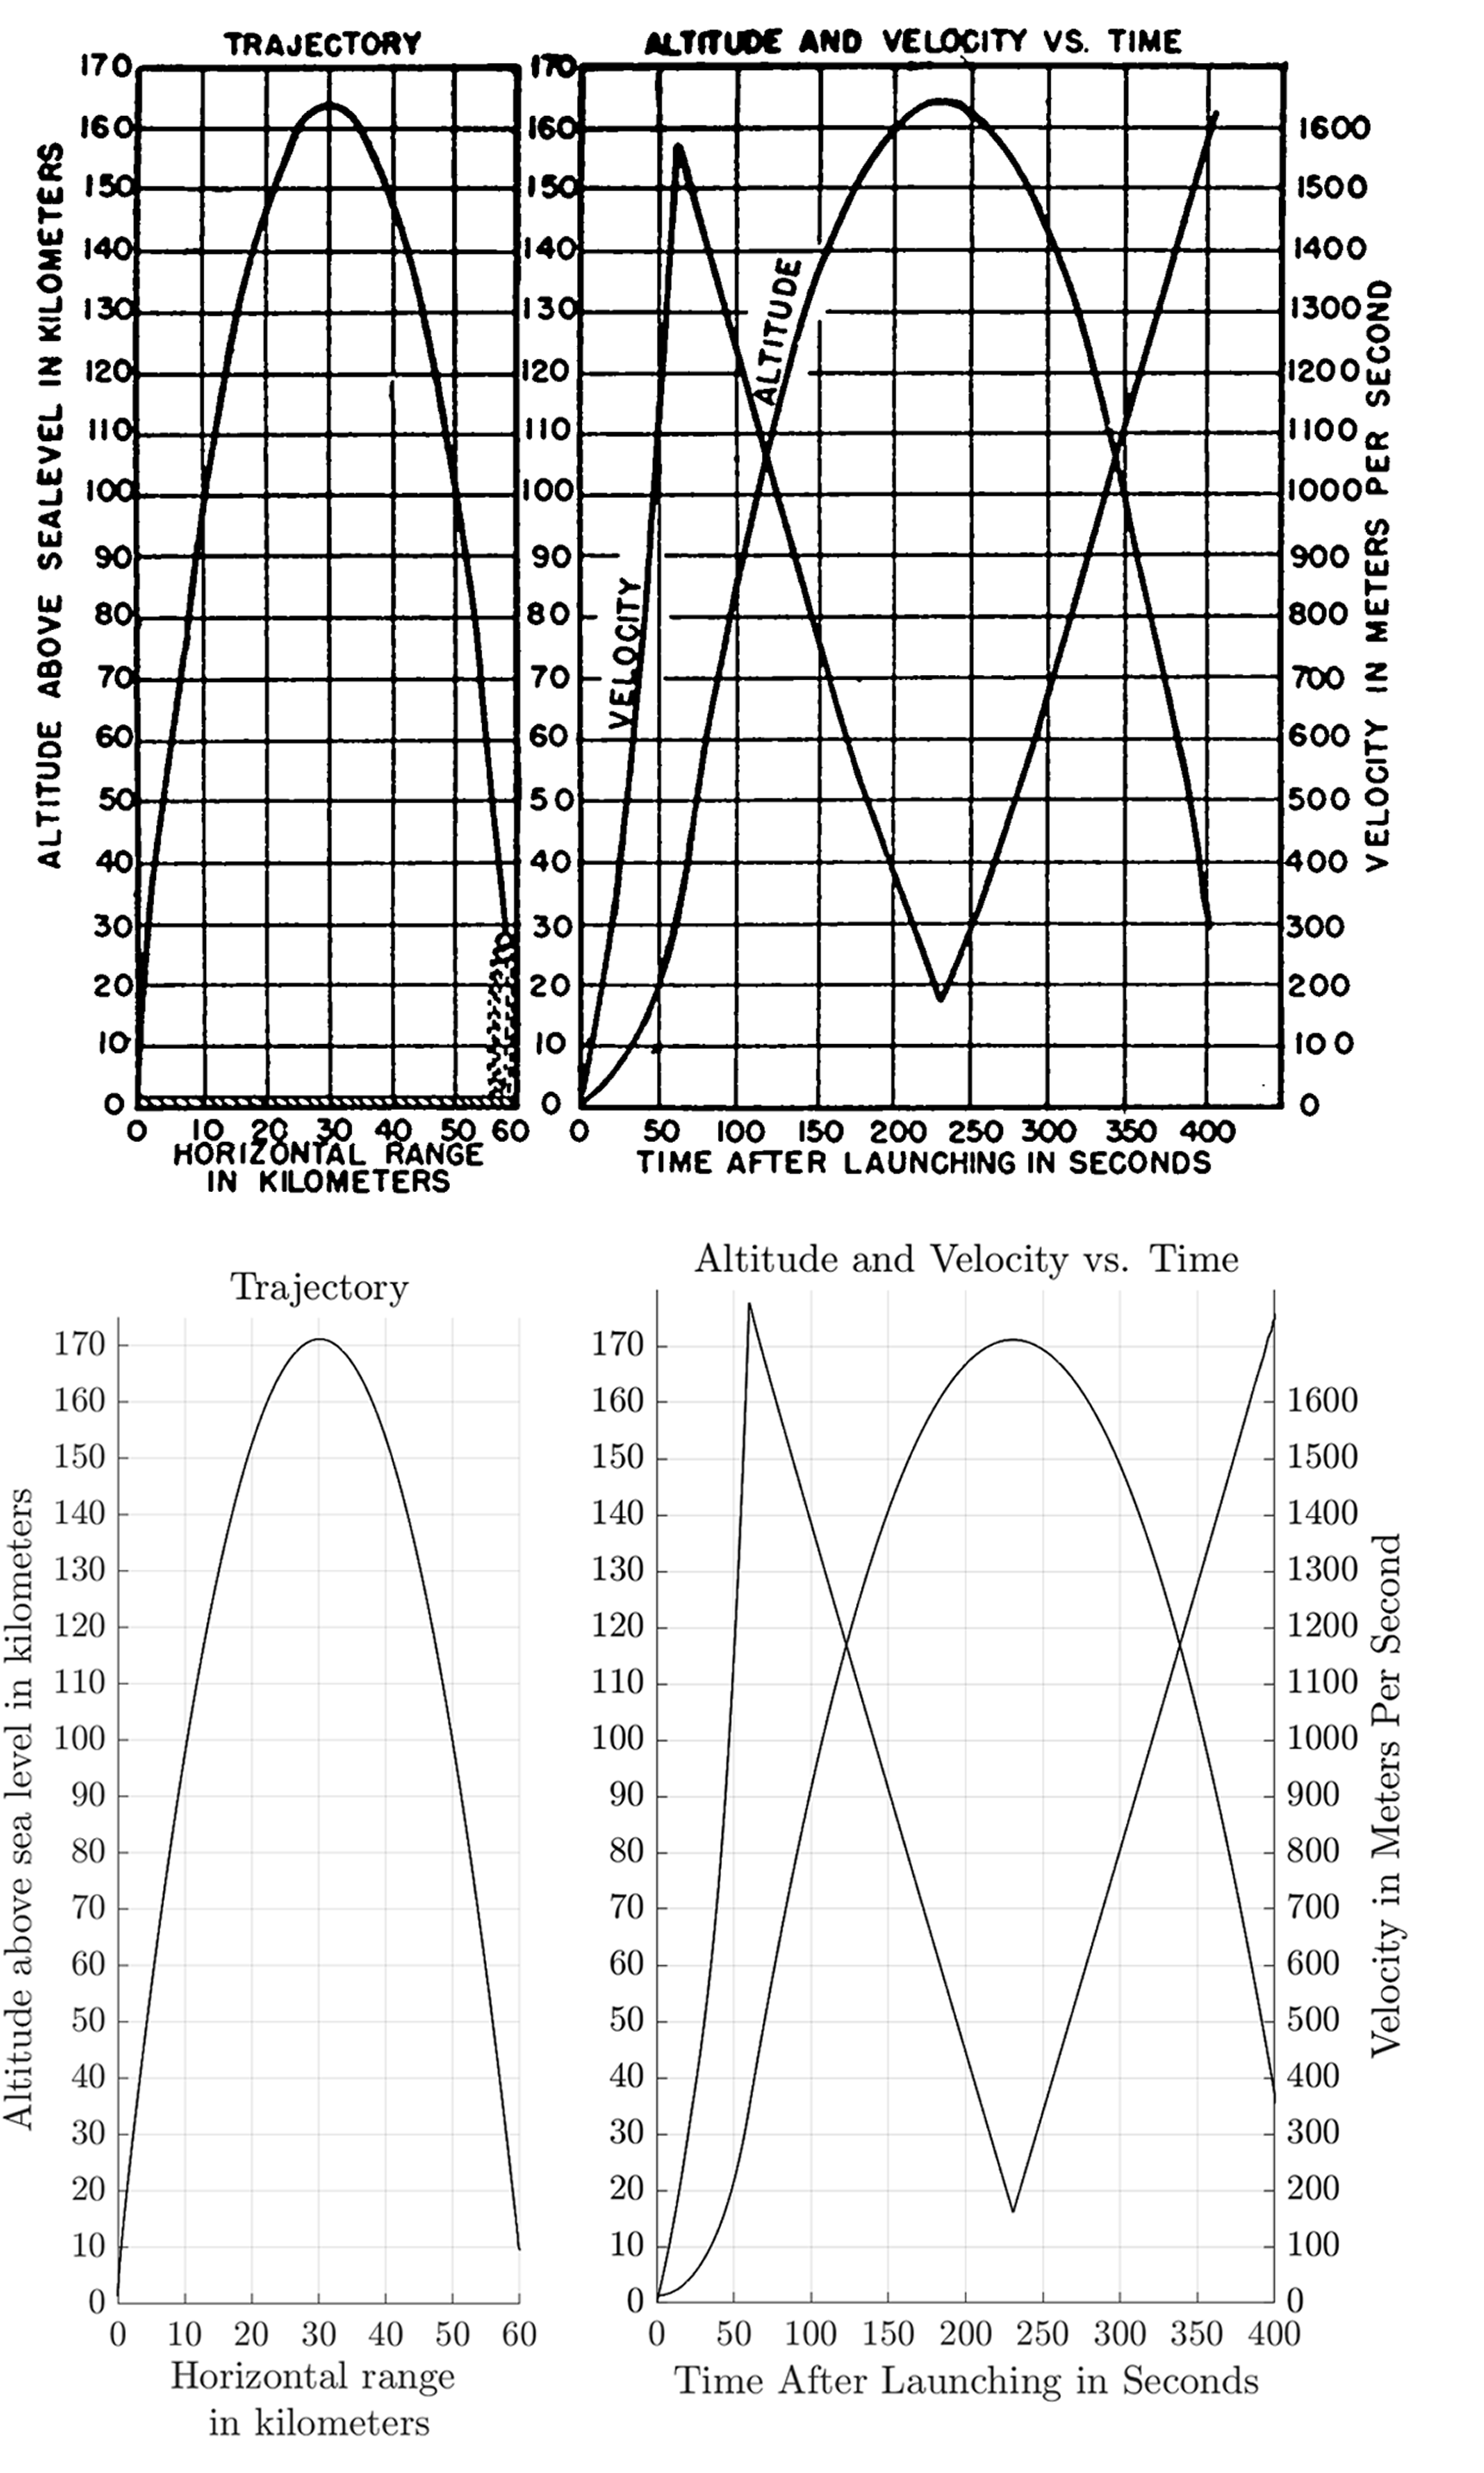
\includegraphics[width=.75\linewidth]{Images/V2 Combined.png}
    \caption{Comparison of Real V-2 Rocket Launch Data against 6-DoF Modeling}
    \label{fig:V2 sim}
\end{figure}


\section{Data Visualization}
Here, we will briefly discuss data visualization and best practices for MATLAB. No matter how good your simulation is, you must be able to appropriately share data in a way that is not only easily conveyed to a non-expert audience, but also visually interesting and descriptive.

At the most basic level, your MATLAB plots should have proper formatting. The default MATLAB plot formatting isn't up to snuff with the standards of scientific publications or presentation of your work. Luckily, MATLAB has many tools to improve the presentation of figures.

MATLAB has the ability for plots to utilize LaTeX formatting for figures. We highly recommend to enable this option for all plots as it allows for much better formatting on figures. This can be done with the following commands:
\begin{lstlisting}[style=Matlab-editor]
set(groot, 'defaultAxesTickLabelInterpreter','latex');
set(groot, 'defaultLegendInterpreter','latex');
set(groot, 'defaultTextInterpreter', 'latex')
\end{lstlisting}
\subsection{Changing Default MATLAB Plotting}
If you want to have these changes to figures universally applied in MATLAB, you can create a file in MATLAB called 'startup.m' that is run when MATLAB is opened. This file must exist in the user path for MATLAB. To find the user path for MATLAB, the command "userpath" can be typed into the command line. This will output something like:
\\
"C:\Users\YourName\OneDrive\Documents\MATLAB"

The code in Listing \ref{code:startup} is the d efault plotting used in this document, which should be a good baseline for professional plots.
\lstinputlisting[style=Matlab-editor, caption = Startup File for Plotting]{startup.m}\label{code:startup}

And with that, we have completed the first Volume of the Flighy Dynamics Bible. Additional information and code can be found in the Appendix. If you have any questions, concerns, or suggestions, feel free to reach out to Hudson Reynolds on Slack or via email at Hudsonj.reynolds@gmail.com


\chapter{Appendix}

\section{Proofs and Derivations}\label{sec:ProofsAndDerivations}
\subsection{Buckingham Pi}\label{Buckingham Pi Deriv}

\begin{center}
$\begin{array}{ccc}
     \text{Variable} & \text{Dimension}
     &  \\ \rho & \frac{M}{L^3}
     &  \\ V    & \frac{L}{T}
     &  \\ S    & L
     &  \\\mu &  \frac{M}{LT}
     &  \\a & \frac{L}{T}
     & \\\alpha & -
\end{array}$
\end{center}

For \gls{buck pi}, we want to select repeating variables that span the base dimensions and do not want to select two variables that have the same dimensions. Somewhat arbitrarily, we select $p$, $V$, and $S$ as the 3 repeating variables.

With each $\Pi$ group, we solve by equating the exponents of the expressions to zero. For example:
$$\Pi_1=\rho^aV^bS^c\mu=M^0L^0T^0$$
Plugging in the dimension of each of these:
$$\Pi_1=\left[\frac{M}{L^3}\right]^a\left[\frac{L}{T}\right]^b[L]^c\left[\frac{M}{LT}\right]=M^0L^0T^0$$
This yields a system of equations with three equations:
\begin{gather}
    M:a+1=0\\L:-3a+b+c-1=0\\T:-b-1=0
\end{gather}
Solving this system gives $a=b=c=-1$. Plugging in these values for the coefficients, we arrive at:
$$\Pi_1=\frac{\mu}{\rho VS}$$
Which is $\frac{1}{Re}$.  The same analysis is done for the rest of the $\Pi$ groups:
\begin{gather}
    \Pi_1=\frac{\rho VS}{\mu}\\
    \Pi_2=\frac{V}{a}\\
    \Pi_3=\frac{F}{\rho V^2S}\\
    \Pi_4=\alpha
\end{gather}
\subsection{Equivalence of Newtonian and Lagrangian Mechanics}\label{equiv newt and lang}

\begin{proof}
We start with Lagrange's equations in rectilinear coordinates $x_i=x,y,z$:

$$\frac{\partial L}{\partial x_i}-\frac{d}{dt}\frac{\partial L}{\partial \dot{x}_i}=0 $$

We know that the \gls{Lagrangian} is given as $L=T-U$, so we can express the Euler-Lagrange equations as:

$$\frac{\partial (T-U)}{\partial x_i}-\frac{d}{dt}\frac{\partial (T-U)}{\partial \dot{x}_i}=0$$

We know that the translational kinetic energy is a function of the velocity only, so $\frac{\partial T}{\partial x_i}=0$. A conservative potential is a function of the position only, so $\frac{\partial U}{\partial \dot{x}_i}=0$. This simplifies the Euler-Lagrange Equation to:
$$-\frac{\partial U}{\partial x_i}=\frac{d}{dt}\frac{\partial T}{\partial \dot{x}_i}$$
For a conservative system, $-\frac{\partial U}{\partial x_i}=F_i$, because the force is the gradient of the potential function.

We know the kinetic energy is given as $\frac{1}{2}m\dot{x}^2$. The derivative with respect to the velocity $\dot{x}$ is $m\dot{x}_i$. Taking the time derivative, we have $\frac{d}{dt}(m\dot{x}_i)=m\ddot{x}_i$ in the case of constant mass (or more generally,  $\frac{d}{dt}(m\dot{x}_i)=\dot{p}_i$).

So, we have $F=m\ddot{x}_i$.

\end{proof}
\begin{corollary}
    From the proof, we can also see that the validity is dependent on the choice of rectangular coordinates. 

    It can further be shown that the Newtonian derivation must be performed in an inertial frame.
\end{corollary}


\section{Code}
This section contains lengthier segments of example code from either the 6-\gls{dof} itself or a proof/example relating to it. Refer to the section numbers to find the appropriate implementation of each code segment.
\subsection{Lorenz Attractor RK4 Example}\label{sec:Lorenz Attractor RK4 Example}
\lstinputlisting[style=Matlab-editor, caption = Lorenz Attractor]{6DoF Explanation Scripts/Lorenz Attractor/LorenzAttractor.m}\label{code:Lorenz}

We also have a script to display the results of this in a nice animation:

\lstinputlisting[style=Matlab-editor, caption =Lorenz Animation]{6DoF Explanation Scripts/Lorenz Attractor/LorenzAnimation.m}\label{code:LorenzAnim}
\subsection{Dzhanibekov Effect Model}
\lstinputlisting[style=Matlab-editor, caption = Dzhanibekov Main]{6DoF Explanation Scripts/Dzhanibekov/DzhanibekovMain.m}\label{code:DzhanMain}

\lstinputlisting[style=Matlab-editor, caption = Dzhanibekov Integrator]{6DoF Explanation Scripts/Dzhanibekov/DzhanibekovIntegrator.m}\label{code:DzhanInt}

\lstinputlisting[style=Matlab-editor, caption = Dzhanibekov Rotation Visualizer]{6DoF Explanation Scripts/Dzhanibekov/RotationsVisualizer.m}\label{code:DzhanRotVis}\


\subsection{Numerical Integration Error Examples}
\lstinputlisting[style=Matlab-editor, caption = Numerical Integration Error Comparison]{6DoF Explanation Scripts/NumericalIntegratorError.m}\label{code:Numerical Error $y'=2t$}

\lstinputlisting[style=Matlab-editor, caption = Numerical Integration of Periodic Function]{6DoF Explanation Scripts/NumericalIntegratorErrorNyquist.m}\label{code:Numerical Error y'=cos(4*pi*t)}
\subsection{6-DoF Code}
The code for the 6-\gls{dof} can be found at \cite{reynolds_hudsonreynoldsflight-dynamics-bible_2025} or accessed via GitHub with the QR code. This GitHub also contains the most up-to-date version of this pdf document:

\begin{figure}[ht]
    \centering
    
\includegraphics[width=0.5\linewidth]{Images/adobe-express-qr-code(1).png}
    \label{fig:qr code}
\end{figure}

\setglossarystyle{altlist}
\printglossary[title=Special Terms, toctitle = Special Terms]

\printbibliography[heading=bibintoc, title={References}]

\end{document}
